\documentclass[a4paper,11pt]{book}
%\documentclass[a4paper,twoside,11pt,titlepage]{book}
\usepackage{listings}
\usepackage{fancyhdr}
\usepackage[utf8]{inputenc}
\usepackage[spanish,es-tabla]{babel}

% \usepackage[style=list, number=none]{glossary} %
%\usepackage{titlesec}
%\usepackage{pailatino}

\decimalpoint
\usepackage{dcolumn}
\newcolumntype{.}{D{.}{\esperiod}{-1}}
\makeatletter
\addto\shorthandsspanish{\let\esperiod\es@period@code}
\makeatother


%\usepackage[chapter]{algorithm}
\RequirePackage{verbatim}
%\RequirePackage[Glenn]{fncychap}
\usepackage{fancyhdr}
\usepackage{graphicx}
\usepackage{rotating}
\usepackage{afterpage}
\usepackage{eurosym}
\usepackage{etoolbox}
\usepackage{textcase}
\usepackage{longtable}
\usepackage{wrapfig}
\usepackage{float}
\usepackage{tcolorbox}

\usepackage[pdfborder={1 1 1}]{hyperref} %referencia

% ********************************************************************
% Re-usable information
% ********************************************************************
\newcommand{\myTitle}{ModernWood\xspace}
\newcommand{\myDegree}{Grado en INGENIERIA INFORMATICA\xspace}
\newcommand{\myName}{Carlos López Martínez\xspace}
\newcommand{\myProf}{Jesús González Peñalver\xspace}
\newcommand{\myOtherProf}{Jesús González Peñalver\xspace}
%\newcommand{\mySupervisor}{Put name here\xspace}
\newcommand{\myFaculty}{Escuela Técnica Superior de Ingenierías Informática y de
Telecomunicación\xspace}
\newcommand{\myFacultyShort}{E.T.S. de Ingenierías Informática y de
Telecomunicación\xspace}
\newcommand{\myDepartment}{Departamento de ...\xspace}
\newcommand{\myUni}{\protect{Universidad de Granada}\xspace}
\newcommand{\myLocation}{Granada\xspace}
\newcommand{\myTime}{\today\xspace}
\newcommand{\myVersion}{Version 0.1\xspace}


\hypersetup{
  pdfauthor = {\texorpdfstring{\myName}{Nombre Alternativo}},
  pdftitle = {\texorpdfstring{\myTitle}{Título Alternativo}},
  pdfsubject = {},
  pdfkeywords = {palabra\_clave1, palabra\_clave2, palabra\_clave3, ...},
  pdfcreator = {LaTeX con el paquete ....},
  pdfproducer = {pdflatex}
}


%\hyphenation{}


%\usepackage{doxygen/doxygen}
%\usepackage{pdfpages}
\usepackage{url}
\usepackage{colortbl,longtable}
\usepackage[stable]{footmisc}
%\usepackage{index}

%\makeindex
%\usepackage[style=long, cols=2,border=plain,toc=true,number=none]{glossary}

% Definición de comandos que me son tiles:
%\renewcommand{\indexname}{Índice alfabético}
%\renewcommand{\glossaryname}{Glosario}

\usepackage[nonumberlist]{glossaries}
\loadglsentries{Glosario/Glosario}
\makenoidxglossaries
% Agrega más entradas según sea necesario


\pagestyle{fancy}
\fancyhf{}
\fancyhead[LO]{\leftmark}
\fancyhead[RE]{\rightmark}
\fancyhead[RO,LE]{\textbf{\thepage}}
\renewcommand{\chaptermark}[1]{\markboth{\textbf{#1}}{}}
\renewcommand{\sectionmark}[1]{\markright{\textbf{\thesection. #1}}}

\setlength{\headheight}{1.5\headheight}

\newcommand{\HRule}{\rule{\linewidth}{0.5mm}}
%Definimos los tipos teorema, ejemplo y definición podremos usar estos tipos
%simplemente poniendo \begin{teorema} \end{teorema} ...
\newtheorem{teorema}{Teorema}[chapter]
\newtheorem{ejemplo}{Ejemplo}[chapter]
\newtheorem{definicion}{Definición}[chapter]

\definecolor{gray97}{gray}{.97}
\definecolor{gray75}{gray}{.75}
\definecolor{gray45}{gray}{.45}
\definecolor{gray30}{gray}{.94}

\lstset{ frame=Ltb,
     framerule=0.5pt,
     aboveskip=0.5cm,
     framextopmargin=3pt,
     framexbottommargin=3pt,
     framexleftmargin=0.1cm,
     framesep=0pt,
     rulesep=.4pt,
     backgroundcolor=\color{gray97},
     rulesepcolor=\color{black},
     %
     stringstyle=\ttfamily,
     showstringspaces = false,
     basicstyle=\scriptsize\ttfamily,
     commentstyle=\color{gray45},
     keywordstyle=\bfseries,
     %
     numbers=left,
     numbersep=6pt,
     numberstyle=\tiny,
     numberfirstline = false,
     breaklines=true,
   }
 
% minimizar fragmentado de listados
\lstnewenvironment{listing}[1][]
   {\lstset{#1}\pagebreak[0]}{\pagebreak[0]}

\lstdefinestyle{CodigoC}
   {
	basicstyle=\scriptsize,
	frame=single,
	language=C,
	numbers=left
   }
\lstdefinestyle{CodigoC++}
   {
	basicstyle=\small,
	frame=single,
	backgroundcolor=\color{gray30},
	language=C++,
	numbers=left
   }

 
\lstdefinestyle{Consola}
   {basicstyle=\scriptsize\bf\ttfamily,
    backgroundcolor=\color{gray30},
    frame=single,
    numbers=none
   }


\newcommand{\bigrule}{\titlerule[0.5mm]}


%CUSTOM CONSOLE STYLE
\usepackage{xcolor}

% Definir colores personalizados
\definecolor{codegreen}{rgb}{0,0.6,0}
\definecolor{codegray}{rgb}{0.5,0.5,0.5}
\definecolor{codepurple}{rgb}{0.58,0,0.82}
\definecolor{backcolour}{rgb}{0.95,0.95,0.95} % Cambiado a un gris claro

\addto\captionsspanish{\renewcommand{\lstlistingname}{Código}}

% Configuración de listings para código de consola
\lstdefinestyle{console}{
    backgroundcolor=\color{backcolour},   
    commentstyle=\color{codegray},
    keywordstyle=\color{codegray},
    numberstyle=\tiny\color{codegray},
    stringstyle=\color{codegray},
    basicstyle=\footnotesize\ttfamily,
    breakatwhitespace=false,         
    breaklines=true,                 
    captionpos=b,                    
    keepspaces=true,                 
    numbers=none,                    
    numbersep=5pt,                  
    showspaces=false,                
    showstringspaces=false,
    showtabs=false,                  
    tabsize=2,
    frame=single,
    moredelim=[is][\textcolor{codepurple}]{|}{|},
}

%Para conseguir que en las páginas en blanco no ponga cabecerass
\makeatletter
\def\clearpage{%
  \ifvmode
    \ifnum \@dbltopnum =\m@ne
      \ifdim \pagetotal <\topskip
        \hbox{}
      \fi
    \fi
  \fi
  \newpage
  \thispagestyle{empty}
  \write\m@ne{}
  \vbox{}
  \penalty -\@Mi
}
\makeatother

\usepackage{pdfpages}
\fancyhf{}
\fancyfoot[C]{\thepage}
\fancyhead[LO,RE]{\leftmark} % Título del capítulo
\fancyhead[LE,RO]{\rightmark} % Título de la sección

\renewcommand{\sectionmark}[1]{\markright{\thesection. \ #1}}  % Activa la configuración de la sección
\renewcommand{\subsectionmark}[1]{\markright{\thesubsection. \ #1}}  % Activa la configuración de la subsección

%Colores para los 
\renewcommand*{\glstextformat}[1]{\textcolor{blue}{#1}}
\hypersetup
{
    colorlinks=true,
    linkcolor={black}, %para el indice
    citecolor={blue},
    urlcolor={black},
    filecolor={black},
    linktoc=all,
}

\newcommand{\glsnocase}[1]{%
  \glsdisp{#1}{\MakeTextLowercase{#1}}%
}

\begin{document}

\begin{titlepage}
\newlength{\centeroffset}
\setlength{\centeroffset}{-0.5\oddsidemargin}
\addtolength{\centeroffset}{0.5\evensidemargin}
\thispagestyle{empty}

\noindent\hspace*{\centeroffset}\begin{minipage}{\textwidth}
\centering

\includegraphics[width=0.9\textwidth]{imagenes/logo_ugr.png}\\[1.4cm]

\textsc{\Large TRABAJO FIN DE GRADO\\[0.2cm]}
\textsc{INGENIERÍA INFORMÁTICA}\\[1cm]
{\Huge\bfseries Diseño y Desarrollo de un Dispositivo de Interfaz Humana\\}
\noindent\rule[-1ex]{\textwidth}{3pt}\\[3.5ex]
{\large\bfseries ModernWood}
\end{minipage}
\vspace{1.5cm}

\noindent\hspace*{\centeroffset}\begin{minipage}{\textwidth}
\centering

\textbf{Autor}\\ {Carlos López Martínez}\\[2.5ex]
\textbf{Directores}\\
Jesús González Peñalver\\[1.5cm]

\begin{center}
\hspace{-3em}
  \begin{minipage}{0.25\textwidth}
    \centering
    
\includegraphics[width=\linewidth]{imagenes/etsiit_logo.png}
  \end{minipage}
  \hspace{1em}
  \vline
  \hspace{3em}
  \begin{minipage}{0.1\textwidth}
    \centering
    \begin{minipage}{1\textwidth}
        
\includegraphics[width=\linewidth]{imagenes/QRGithub.png}
    \end{minipage}%
    \begin{minipage}{1\textwidth}
        Github
    \end{minipage}
  \end{minipage}
\end{center}

\textsc{Escuela Técnica Superior de Ingenierías Informática y de Telecomunicación}\\
\textsc{---}\\
Granada, \today
\end{minipage}
\end{titlepage}
\chapter*{}
%\thispagestyle{empty}
%\cleardoublepage

%\thispagestyle{empty}

\begin{titlepage}
 
\setlength{\centeroffset}{-0.5\oddsidemargin}
\addtolength{\centeroffset}{0.5\evensidemargin}
\thispagestyle{empty}

\noindent\hspace*{\centeroffset}\begin{minipage}{\textwidth}

\centering
%
\includegraphics[width=0.9\textwidth]{imagenes/logo_ugr.jpg}\\[1.4cm]

%\textsc{ \Large PROYECTO FIN DE CARRERA\\[0.2cm]}
%\textsc{ INGENIERÍA EN INFORMÁTICA}\\[1cm]
% Upper part of the page
% 

 \vspace{3.3cm}

%si el proyecto tiene logo poner aquí
\begin{minipage}{1\textwidth}
    
\includegraphics[width=\linewidth]{imagenes/Logo.png}
\end{minipage}%

% Title

\noindent\rule[-1ex]{\textwidth}{3pt}\\[3.5ex]
{\large\bfseries Teclado ISO 105 Español\\[4cm]}
\end{minipage}

\vspace{2.5cm}
\noindent\hspace*{\centeroffset}\begin{minipage}{\textwidth}
\centering

\textbf{Autor}\\ {Carlos López Martínez}\\[2.5ex]
\textbf{Directores}\\
Jesús González Peñalver\\[1.5cm]
%
\includegraphics[width=0.15\textwidth]{imagenes/tstc.png}\\[0.1cm]
%\textsc{Departamento de Teoría de la Señal, Telemática y Comunicaciones}\\
%\textsc{---}\\
%Granada, mes de 201
\end{minipage}
%\addtolength{\textwidth}{\centeroffset}
\vspace{\stretch{2}}

 
\end{titlepage}






\cleardoublepage
\thispagestyle{empty}

\begin{center}
{\large\bfseries Diseño y Desarrollo de un Dispositivo de Interfaz Humana: Teclado ISO 105 Español}\\
\end{center}
\begin{center}
Carlos López Martínez\\
\end{center}

%\vspace{0.7cm}
\noindent{\textbf{Palabras clave}: ISO, PlatformIO, Microcontrolador, ESP32-S3, Bluetooth, Wireless, USB, Windows, Linux}\\

\vspace{0.7cm}
\noindent{\textbf{Resumen}}\\

Creación de un dispositivo de interfaz humana siguiendo el estándar ISO 105 en español. Enfocado en la creación de un dispositivo de interfaz humana, este proyecto se propone diseñar y desarrollar un teclado conforme al estándar ISO 105 en español, ya que no existe gran variedad de estos en el mercado. Para alcanzar este objetivo, se empleará la plataforma "PlatformIO" junto con un microcontrolador ESP32-S3, aprovechando sus capacidades de conectividad y procesamiento. El dispositivo permitirá una interacción con SO Windows y Linux por USB (Cableado) y Bluetooth (Wireless)

Para todo el desarrollo del dispositivo se tendrá en cuenta el coste del mismo, ya que deberá ser abordable, al menos como producto de alta gama, así como se tendrá en cuenta su reparabilidad, estética y en todo momento el rendimiento y funcionamiento.
El dispositivo tiene que funcionar de forma correcta tanto de forma inalámbrica como cableada independientemente, pudiéndose bajar los costes si solo se desea una versión cableada.

El dispositivo dispondrá de una pantalla LCD a color para mostrar información y configuración del mismo, así como código ampliable y su asignación a teclas especiales.
\cleardoublepage


\thispagestyle{empty}


\begin{center}
{\large\bfseries Design and Development of a Human Interface Device: ISO 105 Spanish Keyboard}\\
\end{center}
\begin{center}
Carlos López Martínez\\
\end{center}

%\vspace{0.7cm}
\noindent{\textbf{Palabras clave}: ISO, PlatformIO, microcontroller, ESP32-S3, Bluetooth, Wireless, USB, Windows, Linux}\\

\vspace{0.7cm}
\noindent{\textbf{Abstract}}\\

Creation of a human interface device following the ISO 105 standard in Spanish. Focused on the creation of a human interface device, this project aims to design and develop a keyboard in accordance with the ISO 105 standard in Spanish, as there is not a wide variety of these in the market. To achieve this goal, the "PlatformIO" platform will be used along with an ESP32-S3 microcontroller, taking advantage of its connectivity and processing capabilities. The device will allow interaction with Windows and Linux OS via USB (Wired) and Bluetooth (Wireless).

Throughout the development of the device, its cost will be taken into account, as it must be affordable, at least as a high-end product. Its repairability, aesthetics, and performance and operation will also be considered at all times. The device has to function correctly both wirelessly and wired independently. Costs can be reduced if only a wired version is desired.

The device will have a color LCD screen to display information and configuration of the same. As well as expandable code and its assignment to special keys.

\chapter*{}
\thispagestyle{empty}

\noindent\rule[-1ex]{\textwidth}{2pt}\\[4.5ex]

Yo, \textbf{Carlos López Martínez}, alumno de la titulación INGENIERÍA INFORMÁTICA de la \textbf{Escuela Técnica Superior
de Ingenierías Informática y de Telecomunicación de la Universidad de Granada}, con DNI 20888530E, autorizo la
ubicación de la siguiente copia de mi Trabajo Fin de Grado en la biblioteca del centro para que pueda ser
consultada por las personas que lo deseen.

\vspace{6cm}

\noindent Fdo: Carlos López Martínez

\vspace{2cm}

\begin{flushright}
\today
\end{flushright}


\chapter*{}
\thispagestyle{empty}

\noindent\rule[-1ex]{\textwidth}{2pt}\\[4.5ex]

D. \textbf{Jesús González Peñalver}, Catedrático del departamento de Arquitectura y Tecnología de Computadores de la Universidad de Granada.

\vspace{0.5cm}

\textbf{Informa:}

\vspace{0.5cm}

Que el presente trabajo, titulado \textit{\textbf{Diseño y Desarrollo de un Dispositivo de Interfaz Humana}},
ha sido realizado bajo su supervisión por \textbf{Carlos López Martínez}, y autoriza la defensa de dicho trabajo ante el tribunal
que corresponda.

\vspace{0.5cm}

Y para que conste, expiden y firman el presente informe en Granada a \today

\vspace{1cm}

\textbf{El director:}

\vspace{5cm}

\noindent \textbf{Jesús González Peñalver}

\chapter*{Agradecimientos}
\thispagestyle{empty}

       \vspace{1cm}

A mi familia, por todo el apoyo que me han dado a lo largo de todos
los años. A mis amigos por las ideas y momentos de inspiración. Y a
todos los profesores que me han ayudado y han logrado hacer del Grado de
Ingeniería Informática una gran experiencia.
%\frontmatter
\mainmatter
\tableofcontents
%\listoffigures
%\listoftables
%

\setlength{\parskip}{5pt}

\chapter{Introducción}
\section{Motivación}

Cada vez es más común el uso de ordenadores y sistemas informáticos en todos los ámbitos de la vida, por lo que el uso de dispositivos para poder interactuar con estos también es igual de común. Desde hace muchísimo tiempo, el dispositivo más usado para interactuar con los ordenadores y máquinas a lo largo del mundo es y ha sido el teclado. Existen teclados de todo tipo, formas, distribuciones y tecnologías. Todos ellos con el mismo objetivo, introducir caracteres en el sistema.

Personalmente, desde que puedo recordar siempre he usado el ordenador de casa y he crecido con el teclado de mi lado. He pasado por muchos teclados a lo largo de mi vida y todos ellos han acabado más o menos de la misma forma, estropeados o guardados porque me cansaba del teclado y de como era la sensación al usarlo. Reparar estos teclados era igual de costoso que el propio problema que tenían.

Intente buscar siempre dispositivos que satisficieran mis necesidades, robusto, fácil de arreglar, duraderos, inalámbricos y elegantes. En el mercado existen varios de estos, pero era mi último requisito el que hacía que mi búsqueda no arrojase ningún resultado, que fuera en español. Al fin y al cabo escribo en español y estoy acostumbrado a una distribución española, por lo que dado las exigencias que tengo como usuario y que no hay mercado para lo que busco decidí embarcarme en este proyecto para llenar el hueco que hay en el mercado y satisfacer mis demandas.

Mi desafío no solo radica en encontrar el teclado perfecto para mí, sino también en transformar la concepción convencional de diseño y fabricación de teclados. Para abordar este problema, mi enfoque va más allá de simplemente crear otro dispositivo; mi objetivo es redefinir lo que se considera estándar mediante la implementación de nuevas técnicas y conceptos innovadores.

En lugar de adherirme a las técnicas de fabricación y ensamblaje convencionales, que a menudo resultan en dispositivos difíciles de reparar y poco robustos, planeo adoptar un enfoque disruptivo. La fabricación de la placa de circuito impreso (\gls{PCB}) será un elemento central de esta estrategia. Al diseñar una \gls{PCB} que priorice la facilidad de reparación y la durabilidad, se espera superar las limitaciones de los teclados tradicionales.

La estética del teclado también experimentará un cambio significativo en mi proyecto. En lugar de centrarme únicamente en el aspecto visual, mi enfoque se orientará hacia la funcionalidad y la simplicidad elegante. Esto implica la eliminación de partes estéticas innecesarias para priorizar la funcionalidad y la durabilidad. La forma seguirá a la función, y mi objetivo es crear un teclado que no solo sea una herramienta eficiente, sino también un testimonio de la belleza en la simplicidad.

La modularidad será una característica clave de mi diseño. La capacidad de desmontar y reemplazar fácilmente componentes permitirá a los usuarios personalizar su experiencia según sus necesidades específicas. Desde interruptores hasta placas de circuito, cada elemento será diseñado para ser modular, facilitando tanto la personalización como el mantenimiento.

En términos de conectividad, mi teclado ofrecerá versatilidad. No solo será inalámbrico, aprovechando la comodidad de la tecnología sin cables, sino que también contará con una opción por cable para situaciones donde la estabilidad de la conexión sea prioritaria. Esta dualidad busca ofrecer a los usuarios la flexibilidad necesaria para adaptarse a diferentes entornos y preferencias.

En resumen, mi proyecto busca romper las convenciones establecidas en el diseño y la fabricación de teclados. A través de la implementación de varias tecnologías, un enfoque renovado en la estética, así como la incorporación de características como la modularidad y el diseño simple, aspiro a crear un teclado que no solo satisfaga mis necesidades y pueda llegar a llenar ese vacío en el mercado existente y crear, de una manera u otra, un producto de buena calidad.
\pagebreak

\section{Estado actual de las alternativas}
%Sección
Actualmente, existen muchos teclados, formas, distribuciones, materiales y precios. \cite{cdw-keyboards} Dado que el nuestro, aunque pueda ser fabricado en grandes cantidades, va a ser fabricado como prototipo o una vez. Vamos a mirar las opciones que se conocen como \gls{DIY} o personalizados que son las correspondientes a este tipo de mercado donde se fabrican bajo un precio menos ajustado y en menos cantidades.

En el ámbito de los teclados \gls{DIY} o personalizados, se encuentran diversas opciones que permiten a los usuarios crear su propio dispositivo según sus preferencias y necesidades. Estas alternativas suelen destacar por ofrecer un mayor nivel de personalización en términos de diseño, disposición de teclas, interruptores y retro-iluminación, en comparación con los teclados convencionales o fabricados en masa. \cite{Diy-Keyboard-POPSC}

Una de las opciones más populares para este tipo de teclados son las placas base personalízales. Estas placas permiten a los usuarios seleccionar y soldar sus propios interruptores y estabilizadores, lo que brinda una libertad total en la elección de la disposición de las teclas. Además, suelen admitir la programación de macros y asignación de funciones a través de software.

También existe la posibilidad de elegir interruptores mecánicos específicos siendo una característica clave. Existen diversos tipos de interruptores, como los Cherry MX, Gateron, Kailh, entre otros, cada uno con características únicas en términos de tacto, recorrido y sonoridad. Además, acompañando a estos interruptores, siempre hay lo que se denomina como \gls{Keycaps}, que son los componentes que cubren los interruptores y que al fin y al cabo es lo que el usuario acaba tocando a la hora de escribir en el teclado.

Los teclados personalizados, aunque siempre ofrecen más opciones en cuanto a qué cosas se quieren, también suele conllevar un mayor gasto y por eso es necesario tener en cuenta que se quiere y como pueden cambiar los precios de estos.

%\newpage
\subsection{Conectividad}
En cuanto a conectividad, no hay tanta variedad, ya que esto se refiere a la forma de conectarse a un computador, y por el momento el grueso del mercado y de casi todos los teclados que se usan de forma comercial usan 4 tipos de conexión. 
\newpage
\begin{itemize}
    \item Por Cable \cite{Keyboards-connection-types-wired}
    \begin{itemize}
        \item \gls{USB} \\
            Esta forma de conectividad representa el grueso predominante en la actualidad, ya que prácticamente todos los dispositivos recurren a esta interfaz para establecer conexión con la computadora. Se trata de un estándar en constante evolución, actualizado mediante diversas versiones a lo largo del tiempo.  (\gls{USB} 1.0, \gls{USB} 2.0, \gls{USB} 3.0, \gls{USB} 3.1, \gls{USB} 3.2 ...)
        \item \gls{PS2} \\
            La conexión \gls{PS2} fue ampliamente utilizada en la década de 1990 y principios de la década de 2000 como un estándar para conectar periféricos a computadoras, especialmente dispositivos de entrada como teclados y ratones. Aunque ha sido superada en popularidad por el \gls{USB}, el \gls{PS2} todavía se encuentra en algunos dispositivos más antiguos. Esta interfaz se caracteriza por su conector redondo con pines y ha experimentado varias revisiones a lo largo del tiempo, como el \gls{PS2} estándar y el \gls{PS2} Mini-DIN de 6 pines. A medida que la tecnología ha avanzado, el \gls{PS2} ha quedado en gran medida relegado en favor de interfaces más modernas, pero su legado persiste en sistemas heredados y dispositivos retro. 
    \end{itemize}
    \item Por radiofrecuencia \cite{Keyboards-connection-types-wireless}
    \begin{itemize}
        \item \gls{Bluetooth} \\
            La conectividad por \glsnocase{Bluetooth} ha ganado amplia aceptación en el ámbito inalámbrico, facilitando la comunicación entre dispositivos a corta distancia. Este estándar ha demostrado ser especialmente útil para la conexión de periféricos como auriculares, teclados y ratones de forma inalámbrica. Este estándar también ha ido sufriendo actualizaciones que lo han mejorado en todos sus aspectos. Actualmente casi todos los teclados que son inalámbricos disponen de \glsnocase{Bluetooth}.
    
        \item \gls{Dongle} receptor \\
            El \gls{Dongle} receptor, también conocido como adaptador, desempeña un papel crucial al habilitar la conectividad por radiofrecuencia en dispositivos que no cuentan nativamente con la capacidad \glsnocase{Bluetooth}. Al conectar este pequeño dispositivo, se amplía la gama de dispositivos compatibles y se permite la comunicación inalámbrica. Este se trata de un dispositivo añadido al dispositivo que se conecta a un \gls{USB} y hace de antena receptora, normalmente para un protocolo que no es \glsnocase{Bluetooth} y más especifico a la aplicación, por lo que hace que su \glsnocase{Latencia} y alcance mejoren considerablemente.
    \end{itemize}
\end{itemize}

\subsection{Formatos}

A lo largo de la evolución de los teclados, las configuraciones y disposiciones de las teclas han experimentado cambios significativos para adaptarse a las necesidades cambiantes de los usuarios y a los avances tecnológicos.

Inicialmente, los teclados adoptaron el diseño \gls{QWERTY}, popularizado por las máquinas de escribir y posteriormente estandarizado por IBM. Este diseño se mantiene como el más común en la actualidad.

A lo largo de los años, surgieron alternativas, como el diseño Dvorak, que redistribuye las letras según su frecuencia de uso para aumentar la eficiencia de la escritura.

Para abordar preocupaciones ergonómicas, los teclados divididos surgieron con el objetivo de reducir la tensión al separar el teclado en dos secciones, ya sea físicamente o mediante un diseño ergonómico que coloca las secciones en ángulos más naturales para las manos.

En términos de tamaño y portabilidad, los teclados completos (100\%) ofrecen la disposición estándar, mientras que los teclados Tenkeyless (TKL) eliminan el teclado numérico para reducir el tamaño. Los teclados 75\% reducen aún más el tamaño al ajustar la disposición sin sacrificar funciones esenciales. Luego en el mundo de \gls{DIY} existen variaciones extremas de esto, pudiendo encontrar teclados de 50\%, 45\% y hasta un 35\% que solo disponen de las teclas alfabéticas.

La elección de un formato de teclado se basa en las preferencias y necesidades individuales del usuario, considerando aspectos como la ergonomía, la portabilidad y el uso previsto, ya sea para trabajo, juegos u otros propósitos específicos. \cite{Keyboards-types}

\subsection{Precios}
Cuando se trata de precios, la diversidad en el mercado de teclados refleja una amplia gama de opciones que se adaptan a diferentes presupuestos y necesidades. Desde opciones más asequibles hasta modelos de alta gama, los precios de los teclados varían según diversos factores.

Los teclados estándar con configuraciones tradicionales y cableado suelen ser más asequibles, brindando una opción económica para aquellos con presupuestos más ajustados. Estos teclados son ideales para usuarios que no necesitan características avanzadas o diseños especializados.

En el extremo superior del espectro, los teclados de gama alta ofrecen características avanzadas como retro-iluminación personalizable, interruptores mecánicos de alta calidad, y construcciones premium. Estos modelos suelen apuntar a entusiastas de los juegos, profesionales creativos o usuarios que buscan una experiencia de escritura excepcional.

Además, la introducción de teclados inalámbricos, ergonómicos o compactos también afecta los precios. Los teclados ergonómicos diseñados para reducir la fatiga y mejorar la comodidad pueden tener un costo ligeramente superior, mientras que los modelos inalámbricos ofrecen la ventaja de la movilidad a un precio adicional.

En resumen, la amplia variedad de teclados disponibles en el mercado garantiza que haya opciones para todos los presupuestos. La clave está en identificar las características prioritarias y el uso previsto para encontrar el equilibrio perfecto entre funcionalidad y precio. \cite{Keyboards-Prices}

\subsection{Otros teclados personalizados}
Siempre pueden haber otra razón para buscar un teclado personalizado, entre ellas podemos encontrar cosas como diseños retro y \glsnocase{Vintage}. Teclados Temáticos o de Edición Limitada. 
O también se hace si se quiere conseguir un objetivo principal, normalmente se quiere conseguir, a parte de todo lo mencionado, objetivos de peso, lograr una funcionalidad extra que un teclado normal no va a proveer o de forma extraordinaria una forma de presumir de las capacidades de fabricación y diseño del autor.
\chapter{Especificación del Sistema}

\section{Requisitos}

% Sección
\subsection{Requisitos funcionales} \label{RequisitosFuncionales}

\subsubsection{Conectividad por cable} \label{DiseñoConectividadCable}
\begin{itemize}
\item \textbf{RF-1:} El teclado deberá poder conectarse mediante un cable \gls{USB} para garantizar la compatibilidad con dispositivos sin capacidad \gls{Bluetooth}.
\item \textbf{RF-2:} Se deberá permitir la conexión y desconexión en caliente (\glsnocase{Hot-Plugging}) a través del cable \gls{USB} sin afectar el rendimiento del teclado.
\end{itemize}

\subsubsection{Conectividad Bluetooth} \label{DiseñoConectividadSinCable}
\begin{itemize}
\item \textbf{RF-3:} El teclado deberá ser capaz de establecer una conexión \gls{Bluetooth} con dispositivos compatibles.
\item \textbf{RF-4:} Deberá admitir el emparejamiento seguro con al menos un dispositivo a la vez.
\item \textbf{RF-5:} Se permitirá la conexión \gls{Bluetooth} mientras el dispositivo esté conectado por cable.
\item \textbf{RF-6:} Se permitirá la opción de apagar completamente el \gls{Bluetooth} del dispositivo.
\end{itemize}

\subsubsection{Batería/Energía y Alimentación}
\begin{itemize}
\item \textbf{RF-7:} El teclado contará con una batería recargable que proporcionará una autonomía mientras no esté conectado con cable.
\item \textbf{RF-8:} Se deberá incorporar un sistema de carga eficiente que permita recargar la batería mientras el teclado está conectado por cable.
\item \textbf{RF-9:} El teclado será capaz de funcionar mientras se carga para garantizar un uso continuo.
\item \textbf{RNF-10:} El teclado entrará en modo de suspensión automáticamente después de un período de inactividad para conservar energía.
\end{itemize}

\subsubsection{Distribución de Teclas}
\begin{itemize}
\item \textbf{RF-11:} El diseño del teclado seguirá la distribución \gls{ISO} de 105 teclas para cumplir con los estándares internacionales.
\end{itemize}

\subsubsection{Compatibilidad y Configuración}
\begin{itemize}
\item \textbf{RF-12:} El teclado será compatible con los principales sistemas operativos, como \gls{Windows} y \gls{Linux}.
\item \textbf{RF-13:} Deberá ser posible configurar las funciones y asignaciones de las teclas mediante \glsnocase{Firmware}, además la configuración del usuario se deberá guardar entre usos y apagados del teclado.
\end{itemize}

\subsection{Requisitos no funcionales} \label{RequisitosNoFuncionales}

\subsubsection{Estética y Diseño}
\begin{itemize}
\item \textbf{RNF-1:} El diseño del teclado deberá ser estéticamente agradable.
\item \textbf{RNF-2:} La calidad de los materiales utilizados en la fabricación garantizará durabilidad y resistencia al desgaste.
\item \textbf{RNF-3:} El producto será sencillo de montar y desmontar para su limpieza. El mantenimiento debe ser sencillo.
\end{itemize}

\subsubsection{Seguridad}
\begin{itemize}
\item \textbf{RNF-4:} El sistema de emparejamiento \gls{Bluetooth} deberá seguir protocolos de seguridad estándar para evitar accesos no autorizados.
\end{itemize}

\subsubsection{Rendimiento y \gls{Latencia}} \label{DiseñoRendimiento}
\begin{itemize}
\item \textbf{RNF-5:} El teclado garantizará un rendimiento sin demoras perceptibles, manteniendo una baja \glsnocase{Latencia} durante la escritura y la conexión inalámbrica.
\item \textbf{RNF-6:} La respuesta de las teclas será consistente y proporcionará una experiencia de escritura fluida, independientemente de la conexión utilizada (\gls{Bluetooth} o por cable).
\end{itemize}

\subsubsection{Energía y Eficiencia} \label{DiseñoAhorroEnergia}
\begin{itemize}
\item \textbf{RNF-7:} Se implementarán medidas de ahorro de energía para optimizar la duración de la batería.
\end{itemize}

\subsubsection{Interfaz de Usuario} \label{DiseñoInterfazUsuario}
\begin{itemize}
\item \textbf{RNF-8:} La interfaz de usuario debe ser simple de entender y usar.
\end{itemize}

\section{Especificaciones}

% Sección
\subsection{Especificación Hardware}

\subsubsection{Conectividad por cable}
\begin{itemize}
\item La conexión por cable se realizará a través de un conector XS12 de aviación por su robustez y estética para asegurar una conexión estable y un menor desgaste.
\item El conector atornillado a la carcasa tendrá otro cable Micro JST de 4mm para poder separar la placa base de la carcasa de forma sencilla sin tener que desoldar nada.
\end{itemize}

\subsubsection{Conectividad \gls{Bluetooth}}
\begin{itemize}
\item El teclado estará equipado con un módulo \gls{Bluetooth} que permita garantizar una conexión estable.
\item El dispositivo \gls{Bluetooth}, debe poder establecer una conexión de al menos de 5 metros.
\end{itemize}

\subsubsection{Batería y Alimentación} \label{DiseñoBateriaAlimentacion}
\begin{itemize}
\item La batería recargable será de \glsnocase{Ion de litio} de alta capacidad. Que se ubicara en la parte inferior de la placa base.
\item La batería tendrá un conector para poder desconectarla de la placa base.
\end{itemize}

\subsubsection{Distribución de Teclas} \label{DiseñoDistribucion}
\begin{itemize}
\item Las teclas seguirán el estándar \gls{ISO} con disposición \gls{QWERTY} para adaptarse a los usuarios de habla hispana.
\item Se utilizarán interruptores mecánicos de alta calidad para garantizar una respuesta táctil precisa y duradera. La elección del tipo será del usuario por gusto personal.
\end{itemize}

\subsection{Especificación Software} \label{DiseñoSoftware}

\subsubsection{Configuración y Personalización}
\begin{itemize}
\item El \glsnocase{Firmware} del teclado admitirá perfiles personalizados que podrán almacenarse en la memoria interna del dispositivo.
\item El dispositivo permitirá una opción de crear programas completos que se podrán ejecutar en una tecla. Estos se programarán por \glsnocase{Firmware}.
\end{itemize}

\subsubsection{Compatibilidad con Sistemas Operativos}
\begin{itemize}
\item El teclado será compatible con \gls{Windows} y \gls{Linux}, garantizando una experiencia uniforme en diferentes plataformas.
\item En todo momento será \gls{Plug-and-Play} para facilitar la instalación y uso sin necesidad de \glsnocase{Controladores} adicionales.
\end{itemize}

\subsubsection{Actualizaciones de \glsnocase{Firmware}} \label{DiseñoActualizaciones}
\begin{itemize}
\item Se diseñará el \glsnocase{Firmware} del teclado con la capacidad de recibir actualizaciones, permitiendo mejorar la funcionalidad y corregir posibles vulnerabilidades de seguridad.
\item Las actualizaciones podrán aplicarse de manera sencilla mediante con conector para conectar un \gls{USB} A \gls{TTL}.
\end{itemize}

\subsubsection{Indicadores \gls{LED}}
\begin{itemize}
\item Se incluirán 10 \gls{LED}S para uso personalizado del usuario, tanto estético como funcional, para indicar estados de batería o conexión.
\item Los indicadores \gls{LED} serán configurables, permitiendo a los usuarios personalizar la apariencia y comportamiento de los mismos.
\end{itemize}

\section{Planificación}

Esta sección detalla el plan de desarrollo del teclado (\gls{HID}) con conectividad \gls{Bluetooth}, batería y conexión por cable. La planificación aborda las fases clave del proyecto, asignación de recursos y plazos de entrega. Para ello se ha realizado un gráfico de Gantt para poder organizar las diferentes fases del proyecto en hitos a cumplir.

El gráfico de Gantt realizado podemos verlo en la figura \ref{fig:DiagramaGantt} que señala de manera clara y concisa la planificación temporal del proyecto. Esta planificación se ha realizado para poder estimar mejor los tiempos de trabajo y que aspectos serían necesarios tener para poder progresar. Esto nos ayudará a saber en qué punto del proyecto nos encontramos y qué aspectos debemos mejorar para poder cumplir con los plazos establecidos. Además, nos ayudará a saber qué recursos necesitamos, tanto para estimar el coste del proyecto como para saber qué aspecto es necesario terminar antes para poder avanzar en el proyecto.

\begin{sidewaysfigure}
\centering
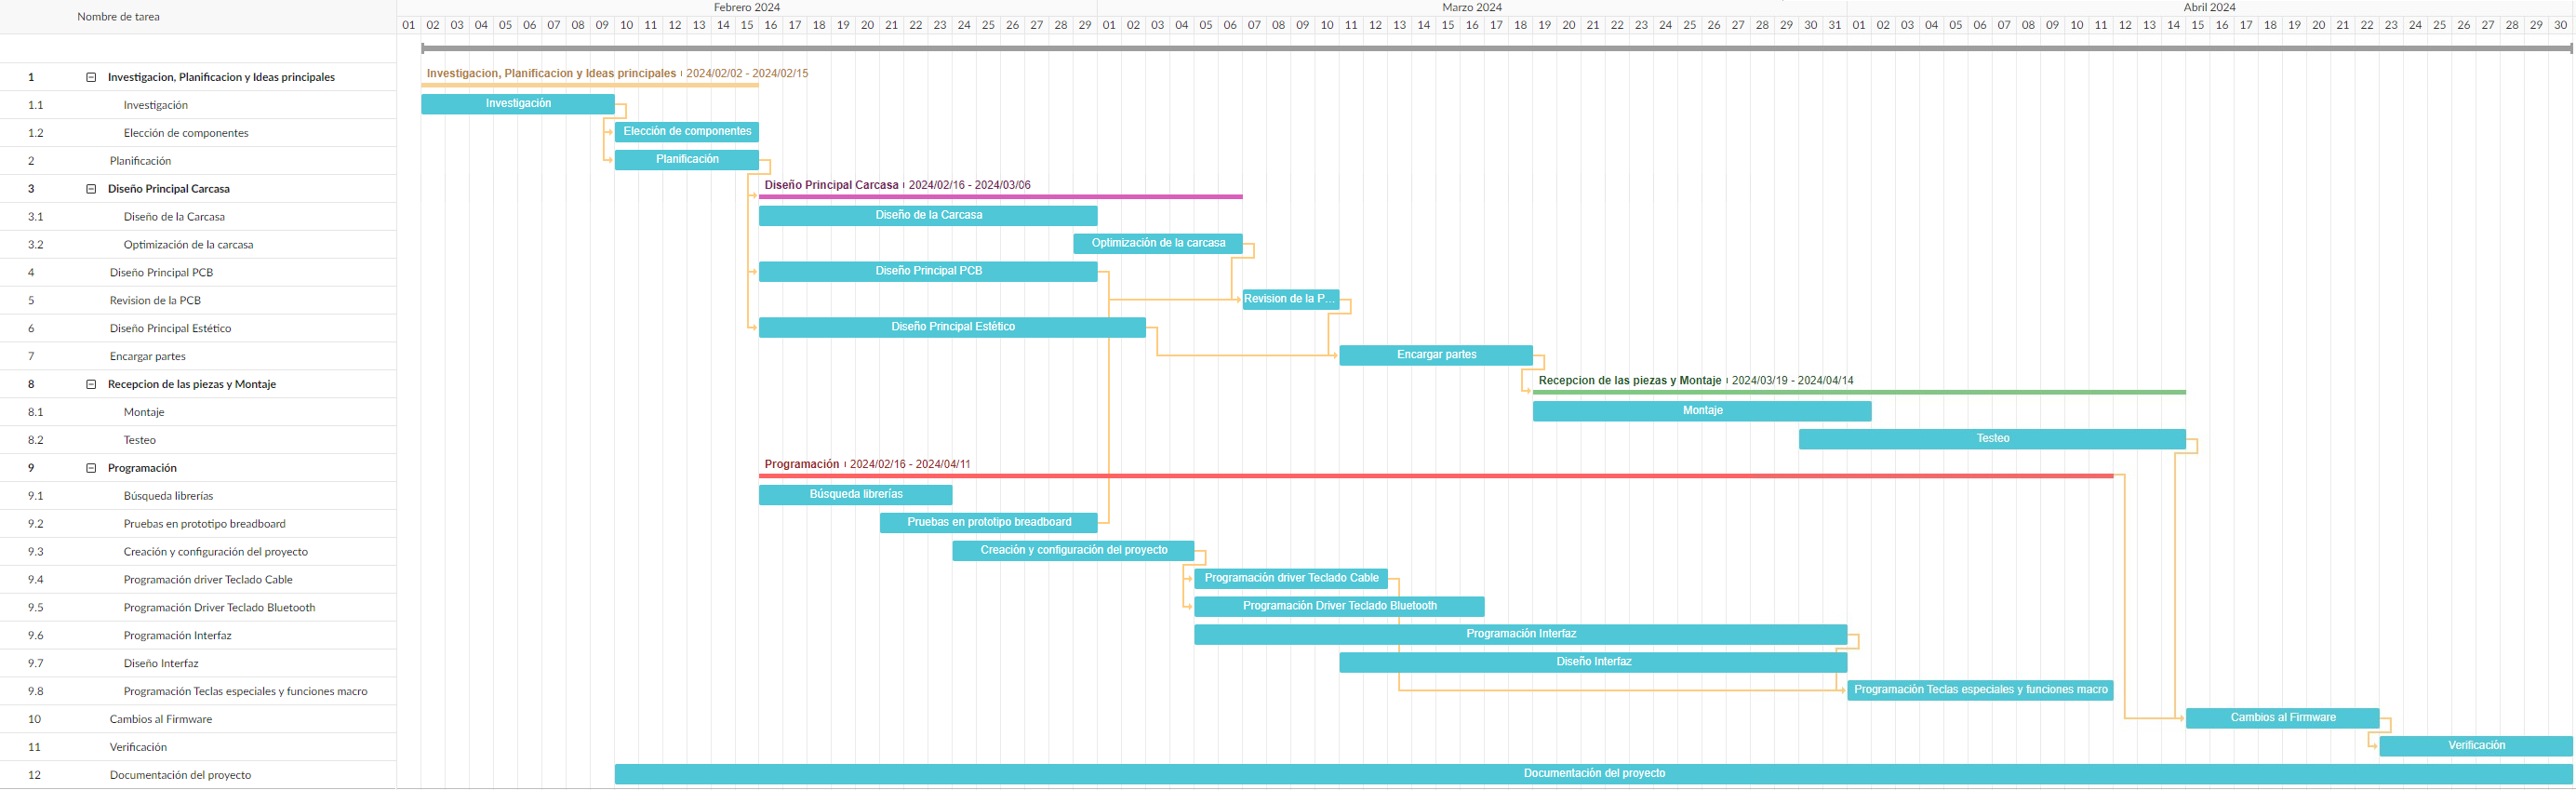
\includegraphics[width=\textheight]{imagenes/Capitulos/Cap02/DiagramaGantt.png}
\caption{Planificación del proyecto con diagrama Gantt.}
\label{fig:DiagramaGantt}
\end{sidewaysfigure}

\input{Capitulos/03_DiseñoyPrototipado}
\chapter{Circuitos}

Como ya se decidió en la sección \ref{Herramientas} se va a usar la herramienta de diseño Eagle.
Usaremos la versión gratuita, ya que las restricciones de esta son en tamaño máximo de la placa. Una vez que tenemos listados los elementos que necesitamos, ya que hemos hecho el diseño previo y sabemos que componentes van a estar presentes, podemos buscar librerías que nos traigan esos componentes para la herramienta Eagle.

\section{Búsqueda de componentes}

Vamos a buscar todos los componentes que van sobre la \gls{PCB}, estos son todos los de la tabla de componentes electrónicos \ref{Table:ComponetesElectronicos} y los interruptores de la tabla de Montaje \ref{Table:ComponentesMontaje}.

\subsubsection{\gls{Multiplexor}}

Para este componente se ha hecho una búsqueda en internet y la página donde se ha encontrado es Snapeda \cite{Snapeda} en la sección de partes podemos hacer una búsqueda y encontramos fácilmente \textbf{74HC154D,653} \cite{SnapedaMux}.

\subsubsection{Condensador}

Para este componente se hizo lo mismo, pero al ser un componente más genérico se puede buscar por el tipo de formato que tiene, ya que hay muchos tipos de formatos para componentes como resistencias y condensadores. En el caso del componente elegido es el formato o paquete 1206, por lo que podemos buscar realmente cualquier condensador con ese tipo de paquete y el valor se lo cambiamos en el programa. En la misma página mencionada anteriormente encontramos el condensador del formato que buscamos \cite{SnapedaCap}.

\subsubsection{Resistencia}

De la misma forma, se ha hecho con la resistencia, en este caso hay varias, pero se han escogido todas del mismo formato para simplificar el trabajo, el formato de la resistencia o paquete es el 0805. En la misma página que las dos anteriores podemos encontrar una resistencia genérica \cite{SnapedaRes}.

\subsubsection{TP4056}

Este si es un chip específico, por lo que la búsqueda va a ser de este chip en concreto. En la misma página SnapEda \cite{Snapeda} encontramos el chip \textbf{TP4056} sin problemas \cite{SnapedaTP4056}.

\subsubsection{DW01A}

En la misma página SnapEda \cite{Snapeda} encontramos el chip \textbf{DW01A} sin problemas \cite{SnapedaDW01A}.

\subsubsection{ME6211C33}

Aunque es un chip específico, tiene un formato muy común, lo que facilita la búsqueda, ya que se corresponde con cualquier regulador de tensión \gls{SMD}. En la misma página SnapEda \cite{Snapeda} encontramos el chip \textbf{LM3940IMP} con el mismo formato que nuestro \textbf{ME6211C33} \cite{SnapedaME6211C33}.

\subsubsection{FS8205A}

Este chip es otro específico por lo que la búsqueda va a ser de este chip en concreto. En la misma página SnapEda \cite{Snapeda} encontramos el chip \textbf{FS8205A} sin problemas \cite{SnapedaFS8205A}.

\subsubsection{ESp32S3} \label{ESp32S3BusquedaComponente}

Este chip es otro específico por lo que la búsqueda va a ser de este chip en concreto. En la misma página SnapEda \cite{Snapeda} encontramos el chip \textbf{ESp32S3} sin problemas, aunque este posteriormente lo vamos a modificar. \cite{SnapedaESp32S3}.

\subsubsection{\gls{LED}S}

En cuanto a los \glsnocase{LED}s podremos encontrar otros de forma genérica, igual que hicimos con las resistencias o condensadores. En la misma página que todo lo anterior podemos encontrarlo de nuevo \cite{SnapedaWS2812B}.

\subsubsection{Diodos}

Como vuelve a ser algo genérico un diodo de paquete SOD-123 podemos buscar cualquier diodo de este formato, aunque el nuestro sea el \textbf{1N5819W}. En la página que hemos usado anteriormente podemos encontrar fácilmente muchos diodos con ese formato \cite{Snapeda1N5819W}.

\subsubsection{Interruptores}

Para los interruptores vamos a prescindir de la página anterior, si no que vamos a buscar de nuevo en internet porque hay una buena comunidad detrás de todo este tipo de dispositivos y será mucho más fácil encontrar lo que necesitamos. En seguida encontramos un repositorio con la librería específica que necesitamos para nuestros interruptores \cite{GitInterruptores}.

\subsection{Creación de componentes}

Como se ha mencionado antes en la subsección de componentes \ref{ESp32S3BusquedaComponente}, vamos a modificar el componente ESP32S3.

La modificación hará que soldar este componente sea más sencillo, ya que facilitará la soldadura \gls{SMD} haciendo que la parte inferior con los pines de soldadura que van pegados a la placa sean visibles desde el otro lado de esta.

\begin{tcolorbox}[colback=blue!5!white, colframe=blue!55!white, title=Nota]
    Ver el apéndice \ref{ApendiceEsp32Hole} para más información sobre el diseño de este componente.
\end{tcolorbox}

\newpage
\section{Diseño Esquemático}
Para el diseño esquemático se han importado todos los componentes a Eagle y se han creado distintas partes del sistema para posteriormente interconectarlas todas en el diseño final.

\begin{tcolorbox}[colback=blue!5!white, colframe=blue!55!white, title=Nota]
    Ver el apéndice \ref{ApendiceDiseñoEsquematico} para más información sobre el diseño esquemático y las consideraciones tomadas. 
\end{tcolorbox}

\subsubsection{Matriz del Teclado}
En esta parte se ha seguido el ejemplo básico que podemos ver en la figura \ref{fig:EjemploArrayTeclado} en el apartado de diseño, donde se opta por una configuración de filas y columnas con su respectivo diodo para evitar \gls{Ghosting}. En la fase de diseño se decidió que iba a ser una matriz de 16*6 teclas únicas, una tecla especial individual y 13 teclas repetidas. La matriz finalmente queda como se muestra en la figura \ref{fig:MatrizTeclas}.

\begin{figure}[H]
    \centering
    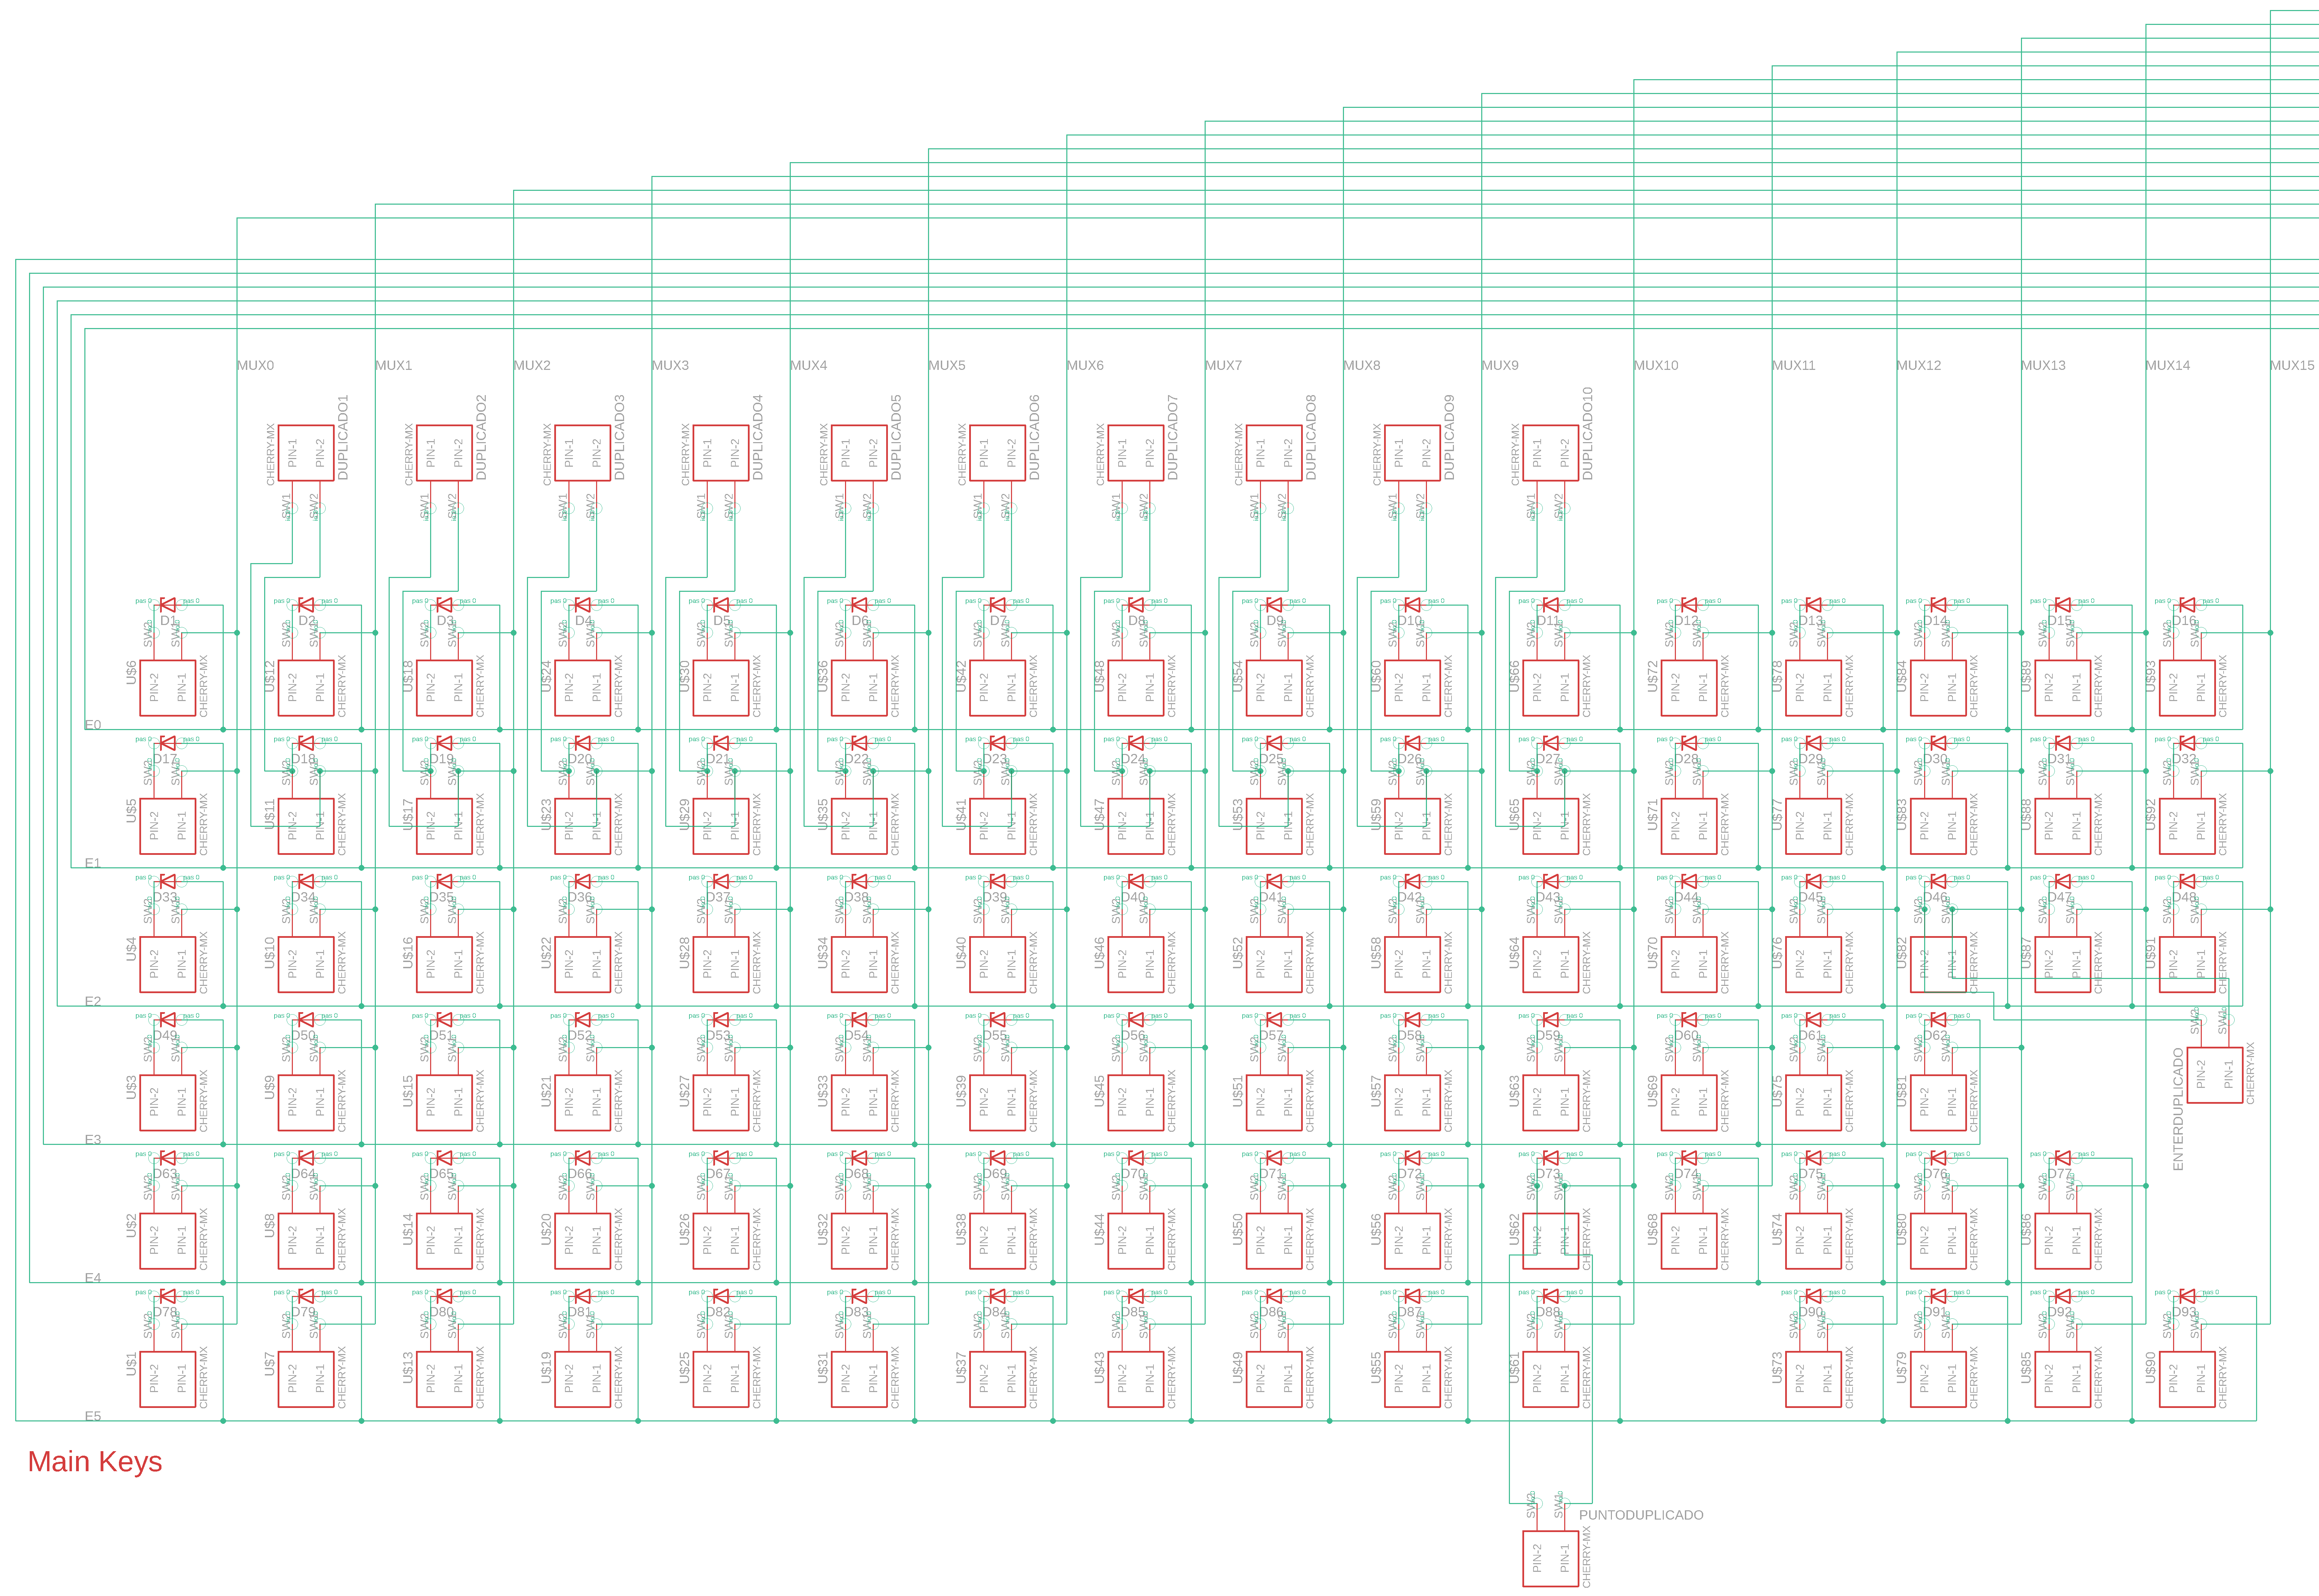
\includegraphics[width=1.0\textwidth]{imagenes/Capitulos/Cap04/MatrizTeclas.png}
    \caption{Matriz final de teclas \cite{Repo:ImagenCircuito}}
    \label{fig:MatrizTeclas}
\end{figure}

\newpage
\subsubsection{\gls{Multiplexor}}
Esta parte se trata de las entradas y salidas del \glsnocase{Multiplexor} hacia la matriz y al microcontrolador. Esta parte es bastante sencilla como se puede apreciar en la figura \ref{fig:MuxImagenCircuito}.

\begin{figure}[H]
    \centering
    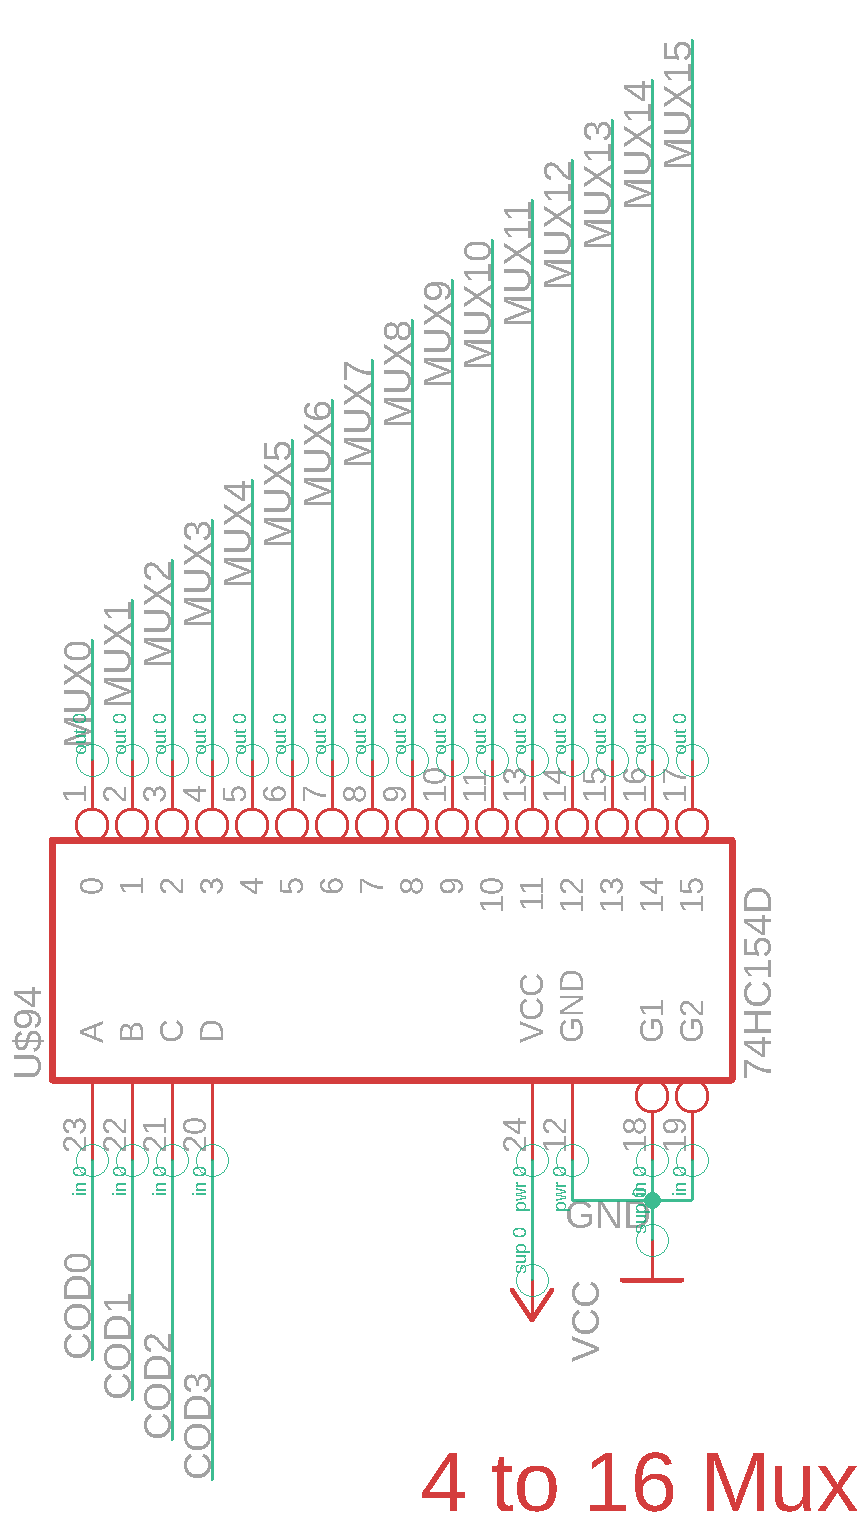
\includegraphics[width=0.6\textwidth]{imagenes/Capitulos/Cap04/Mux.png}
    \caption{\gls{Multiplexor} con todos los pines conectados a sus salidas/entradas \cite{Repo:ImagenCircuito}}
    \label{fig:MuxImagenCircuito}
\end{figure}

\newpage
\subsubsection{Controlador Principal}
Esta parte del circuito es el chip principal (ESP32S3) junto con los botones necesarios para programarla en el momento de subir el firmware, las resistencias que mantienen la placa encendida y la única tecla especial. Todo se puede apreciar en la figura \ref{fig:ESP32S3Circuito}

\begin{figure}[H]
    \centering
    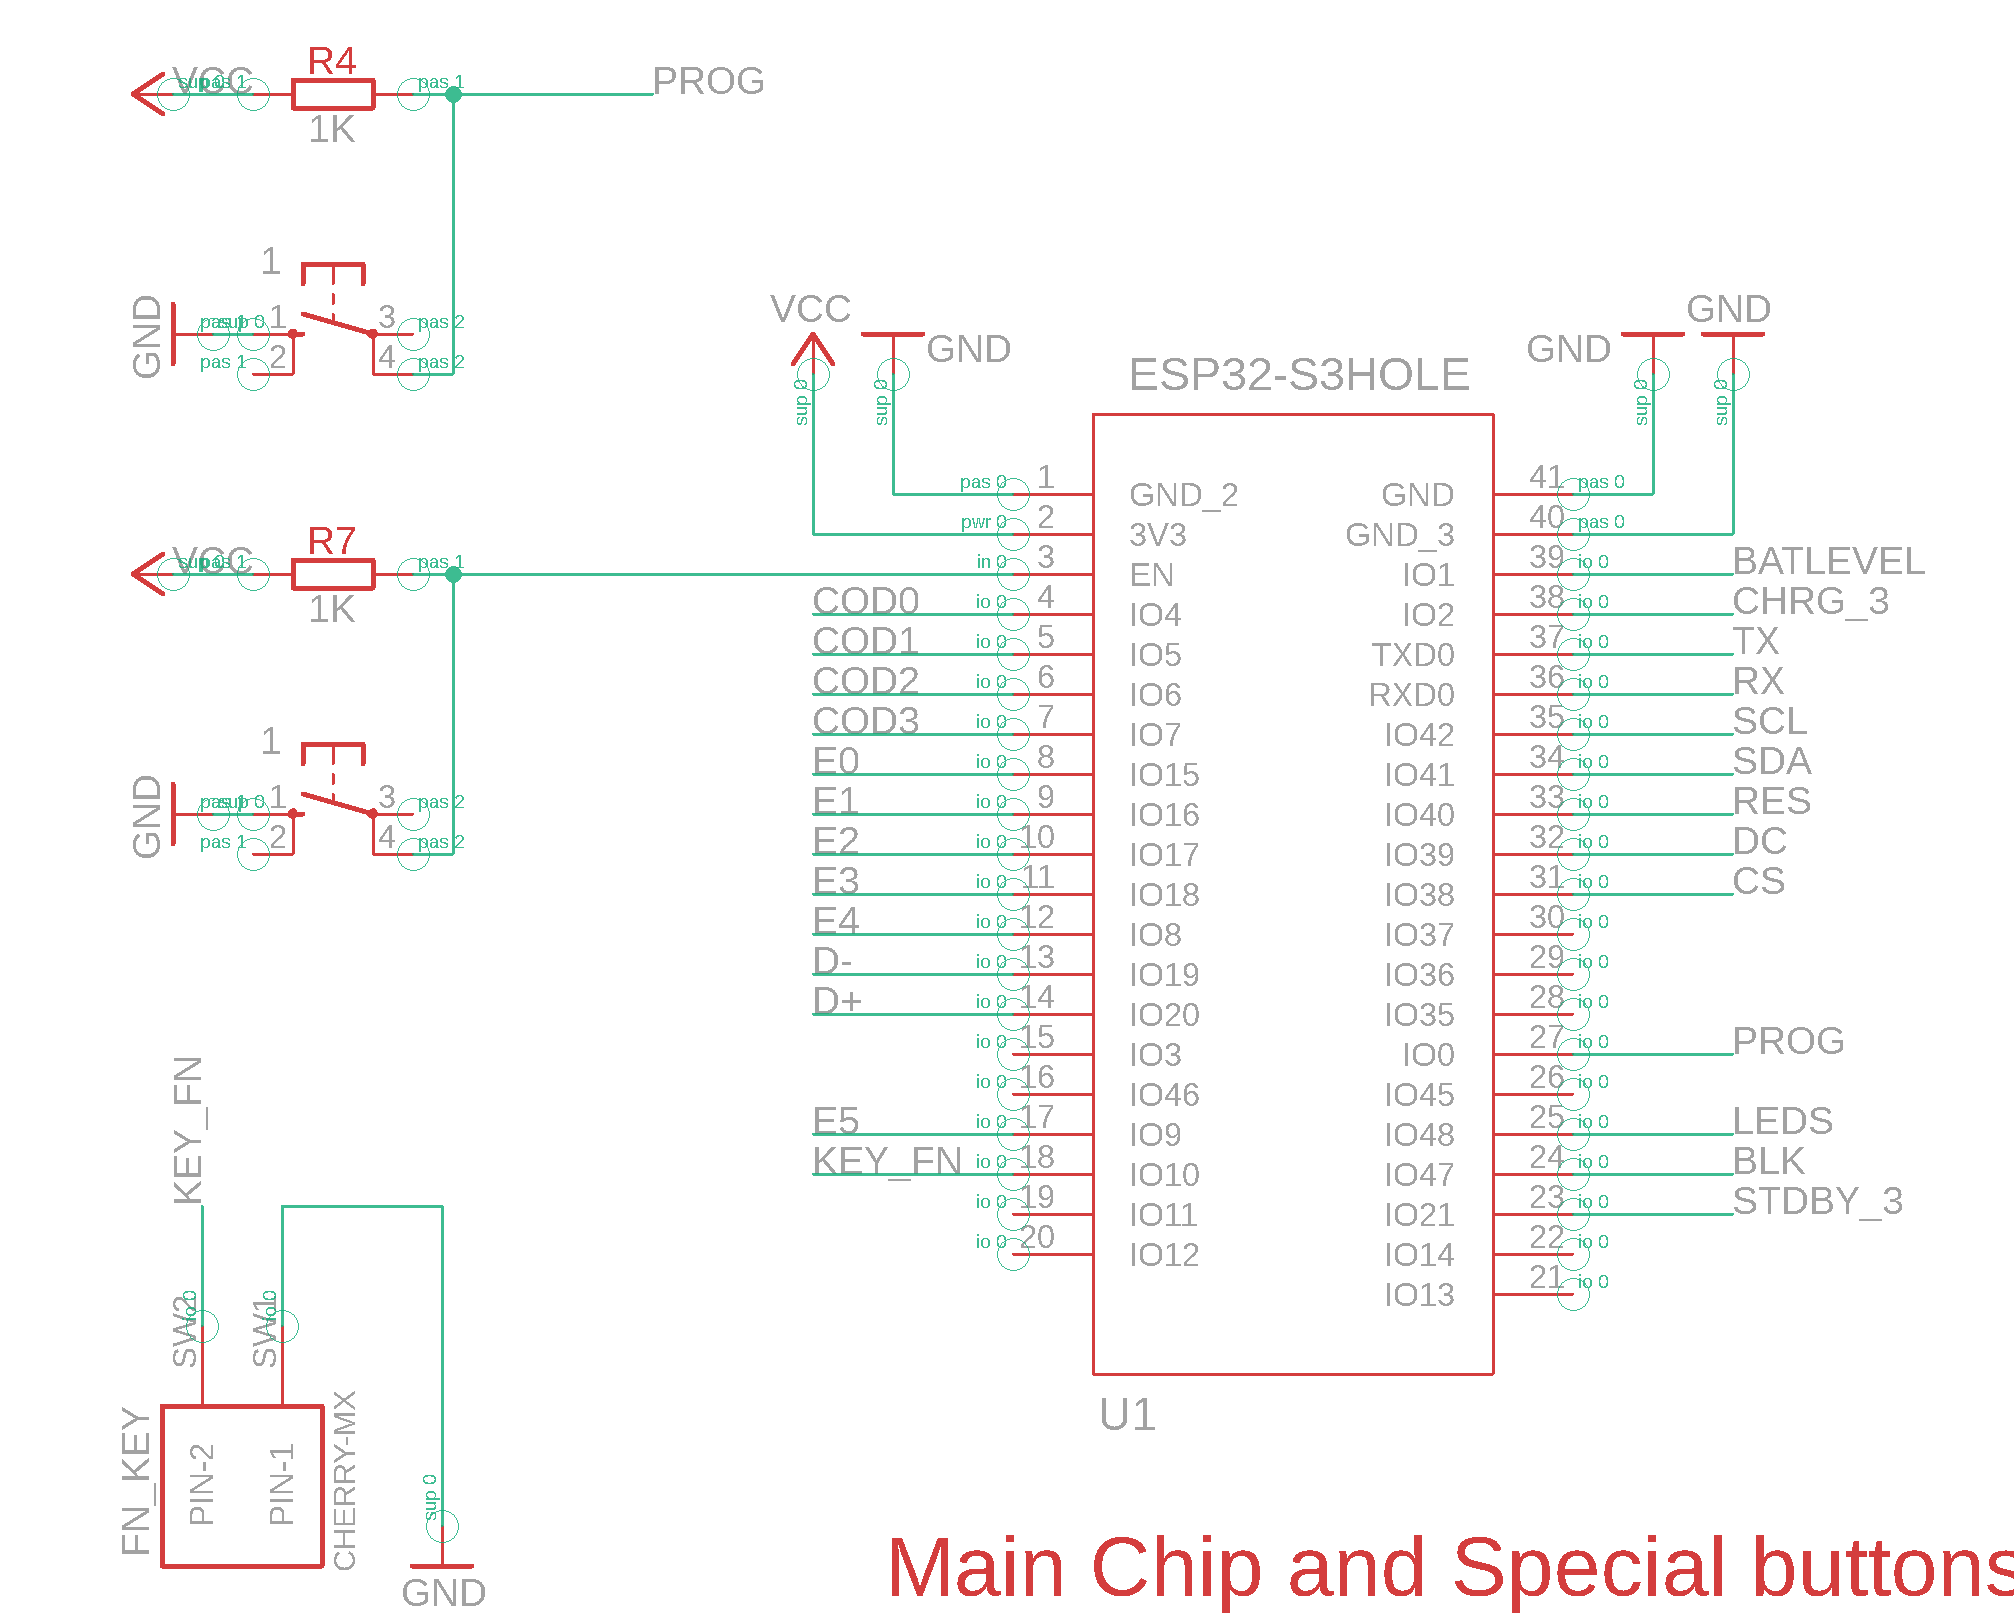
\includegraphics[width=1.0\textwidth]{imagenes/Capitulos/Cap04/CHIP.png}
    \caption{Microcontrolador principal ESP32S3 y tecla principal \cite{Repo:ImagenCircuito}}
    \label{fig:ESP32S3Circuito}
\end{figure}

\newpage
\subsubsection{Bateria y alimentación}
Como este teclado tiene que soportar alimentación por batería a 4.2 V, por \gls{USB} a 5.0 V y a 3.3 V para el ESP32S3 es necesario un circuito que se encargue de estos voltajes, de proteger la batería y proteger todos los circuitos. Se puede ver el circuito encargado de esto en la figura \ref{fig:CircuitoBateriaAlimentacion}. Todo el diseño se ha hecho siguiendo el apartado \ref{InvestigacionSistemaBateria} y la figura \ref{fig:SchemeTP4056}.

\begin{figure}[H]
    \centering
    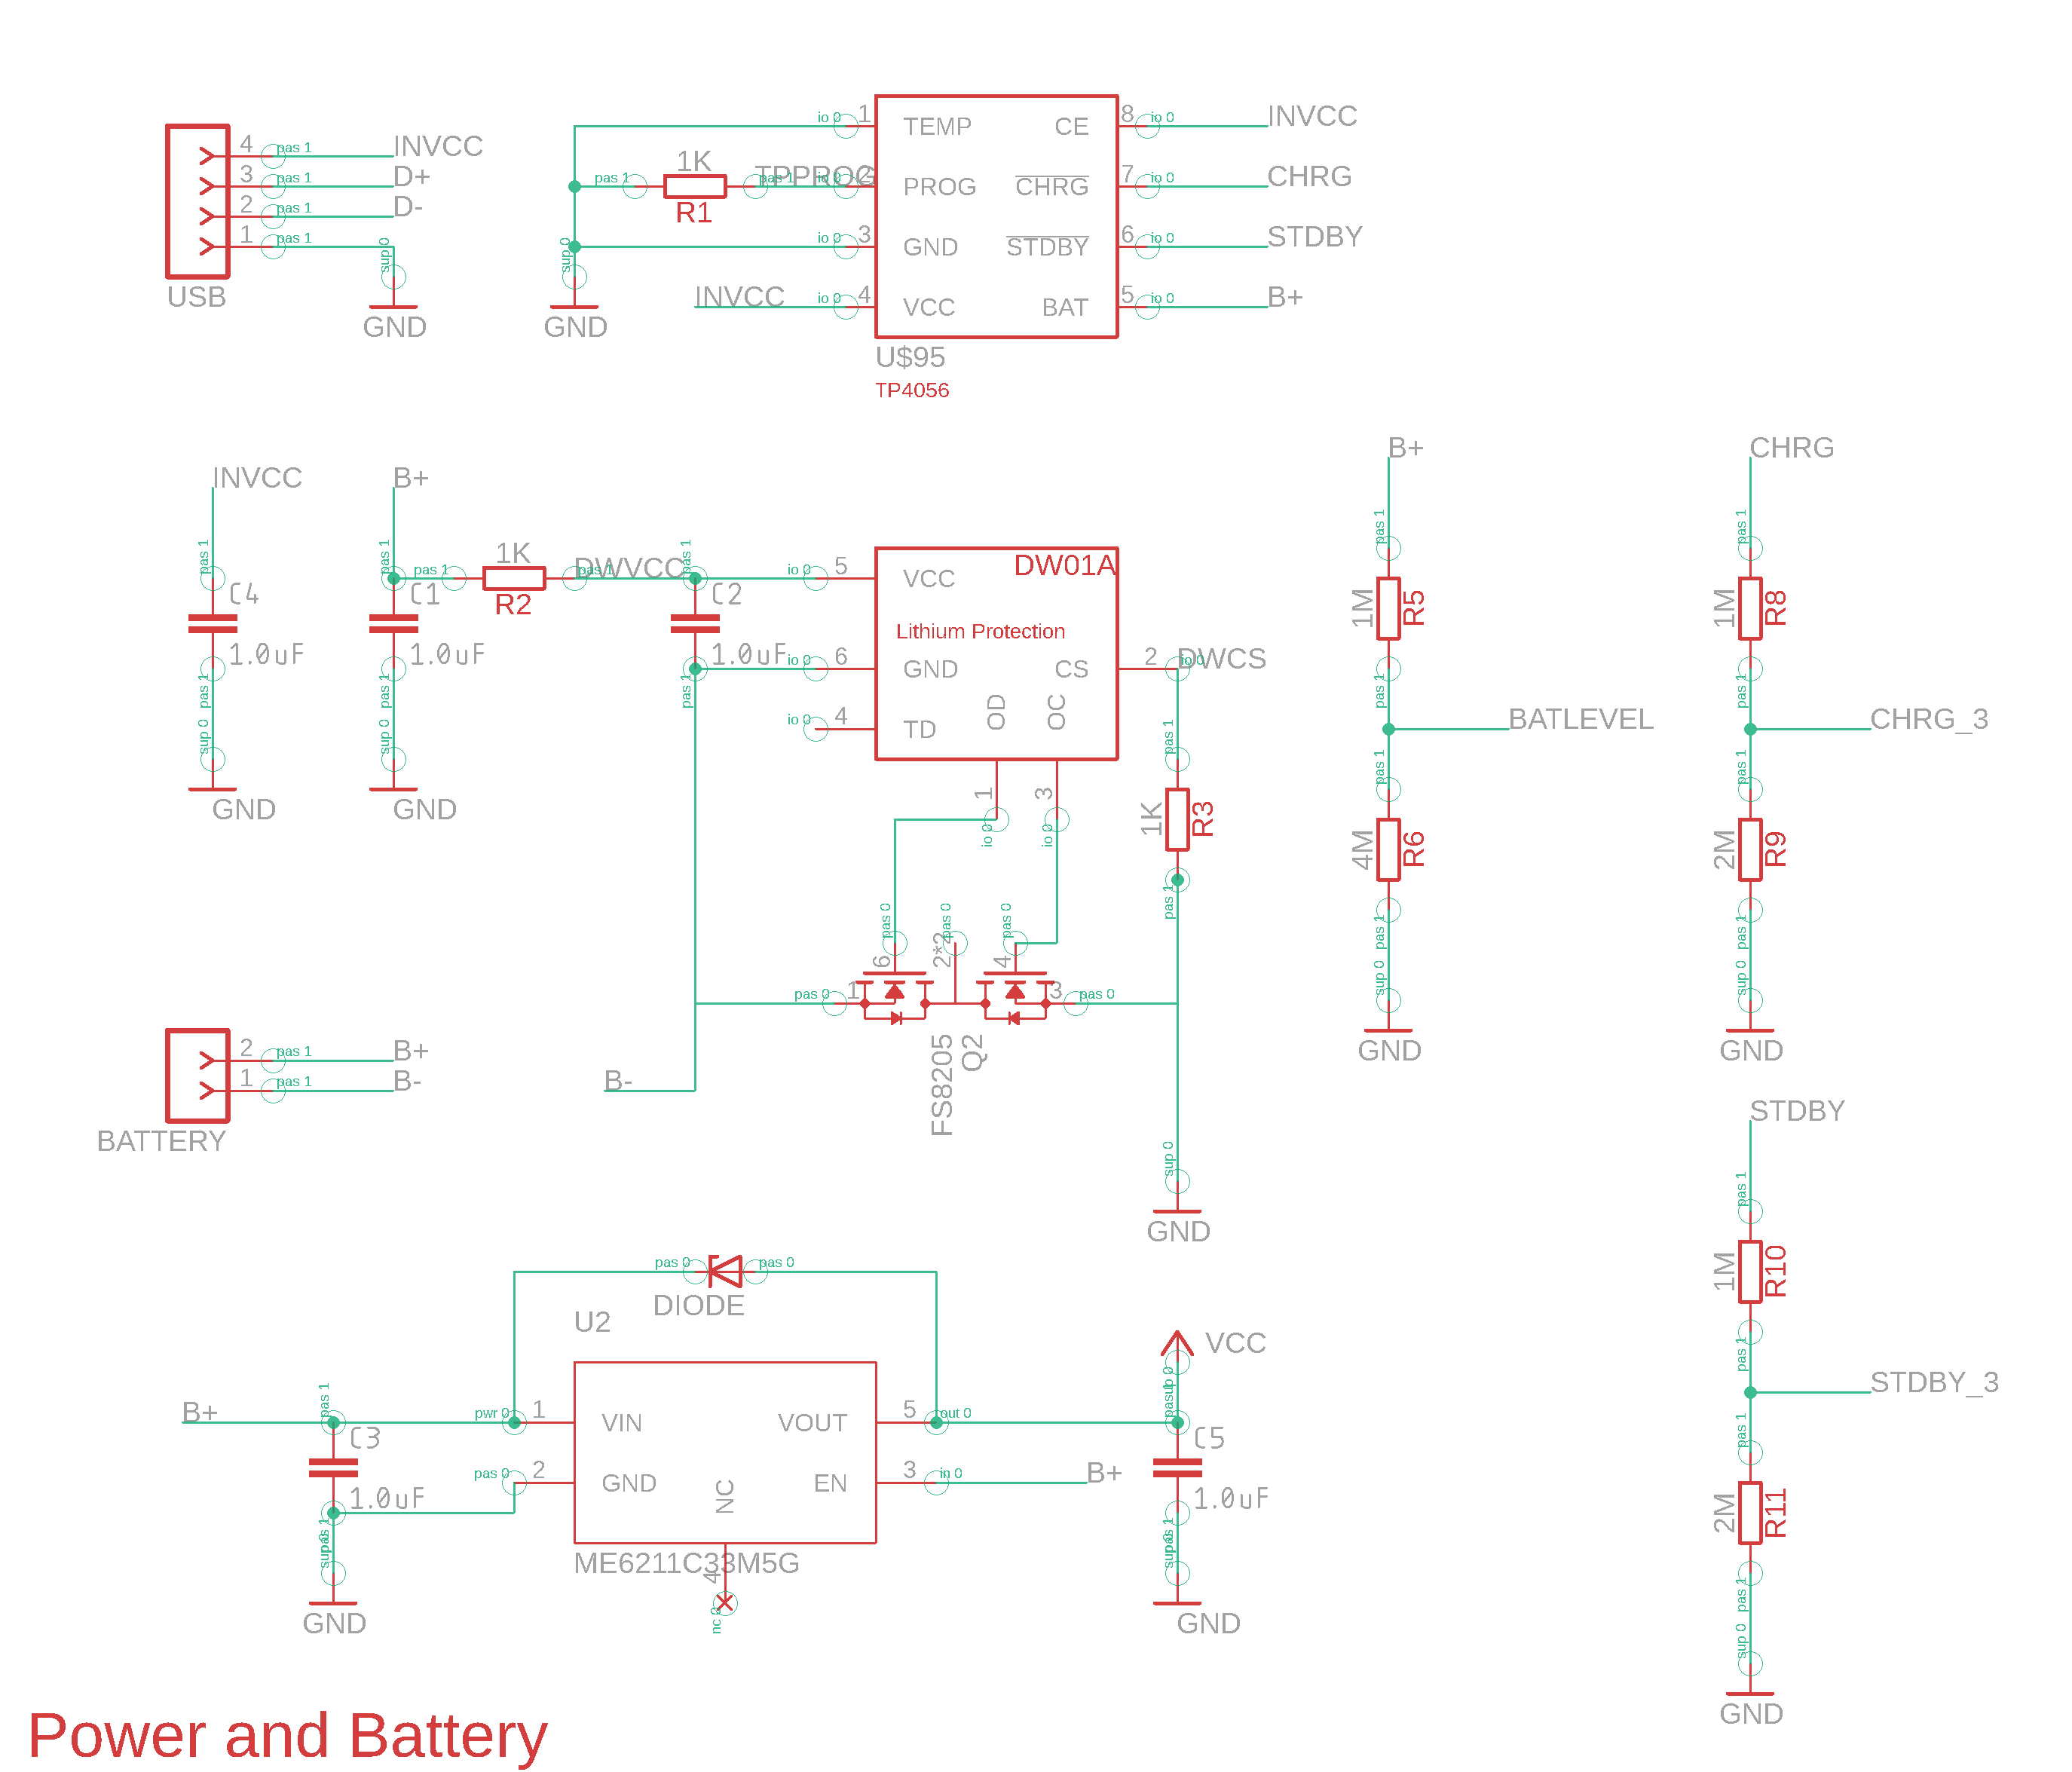
\includegraphics[width=1.0\textwidth]{imagenes/Capitulos/Cap04/Battery.png}
    \caption{Sistema de alimentación y protección del teclado \cite{Repo:ImagenCircuito}}
    \label{fig:CircuitoBateriaAlimentacion}
\end{figure}

\begin{tcolorbox}[colback=red!11!white, colframe=red!50!white, title=Errores]
    Ver apartado de errores \ref{CorrienteInversa} y \ref{VoltajeRegulador} donde se explica por qué se ha añadido un diodo en la puerta del regulador de tensión.
\end{tcolorbox}

\newpage
\subsubsection{\gls{LED}S}
En la fase de diseño, en el punto \ref{DiseñoLeds} se decidió que tuviera \glsnocase{LED}s, ya que eran fáciles de programar y daban mucho juego. El apartado eléctrico de los \glsnocase{LED}s se puede observar en la figura \ref{fig:CircuitoLeds}.

\begin{figure}[H]
    \centering
    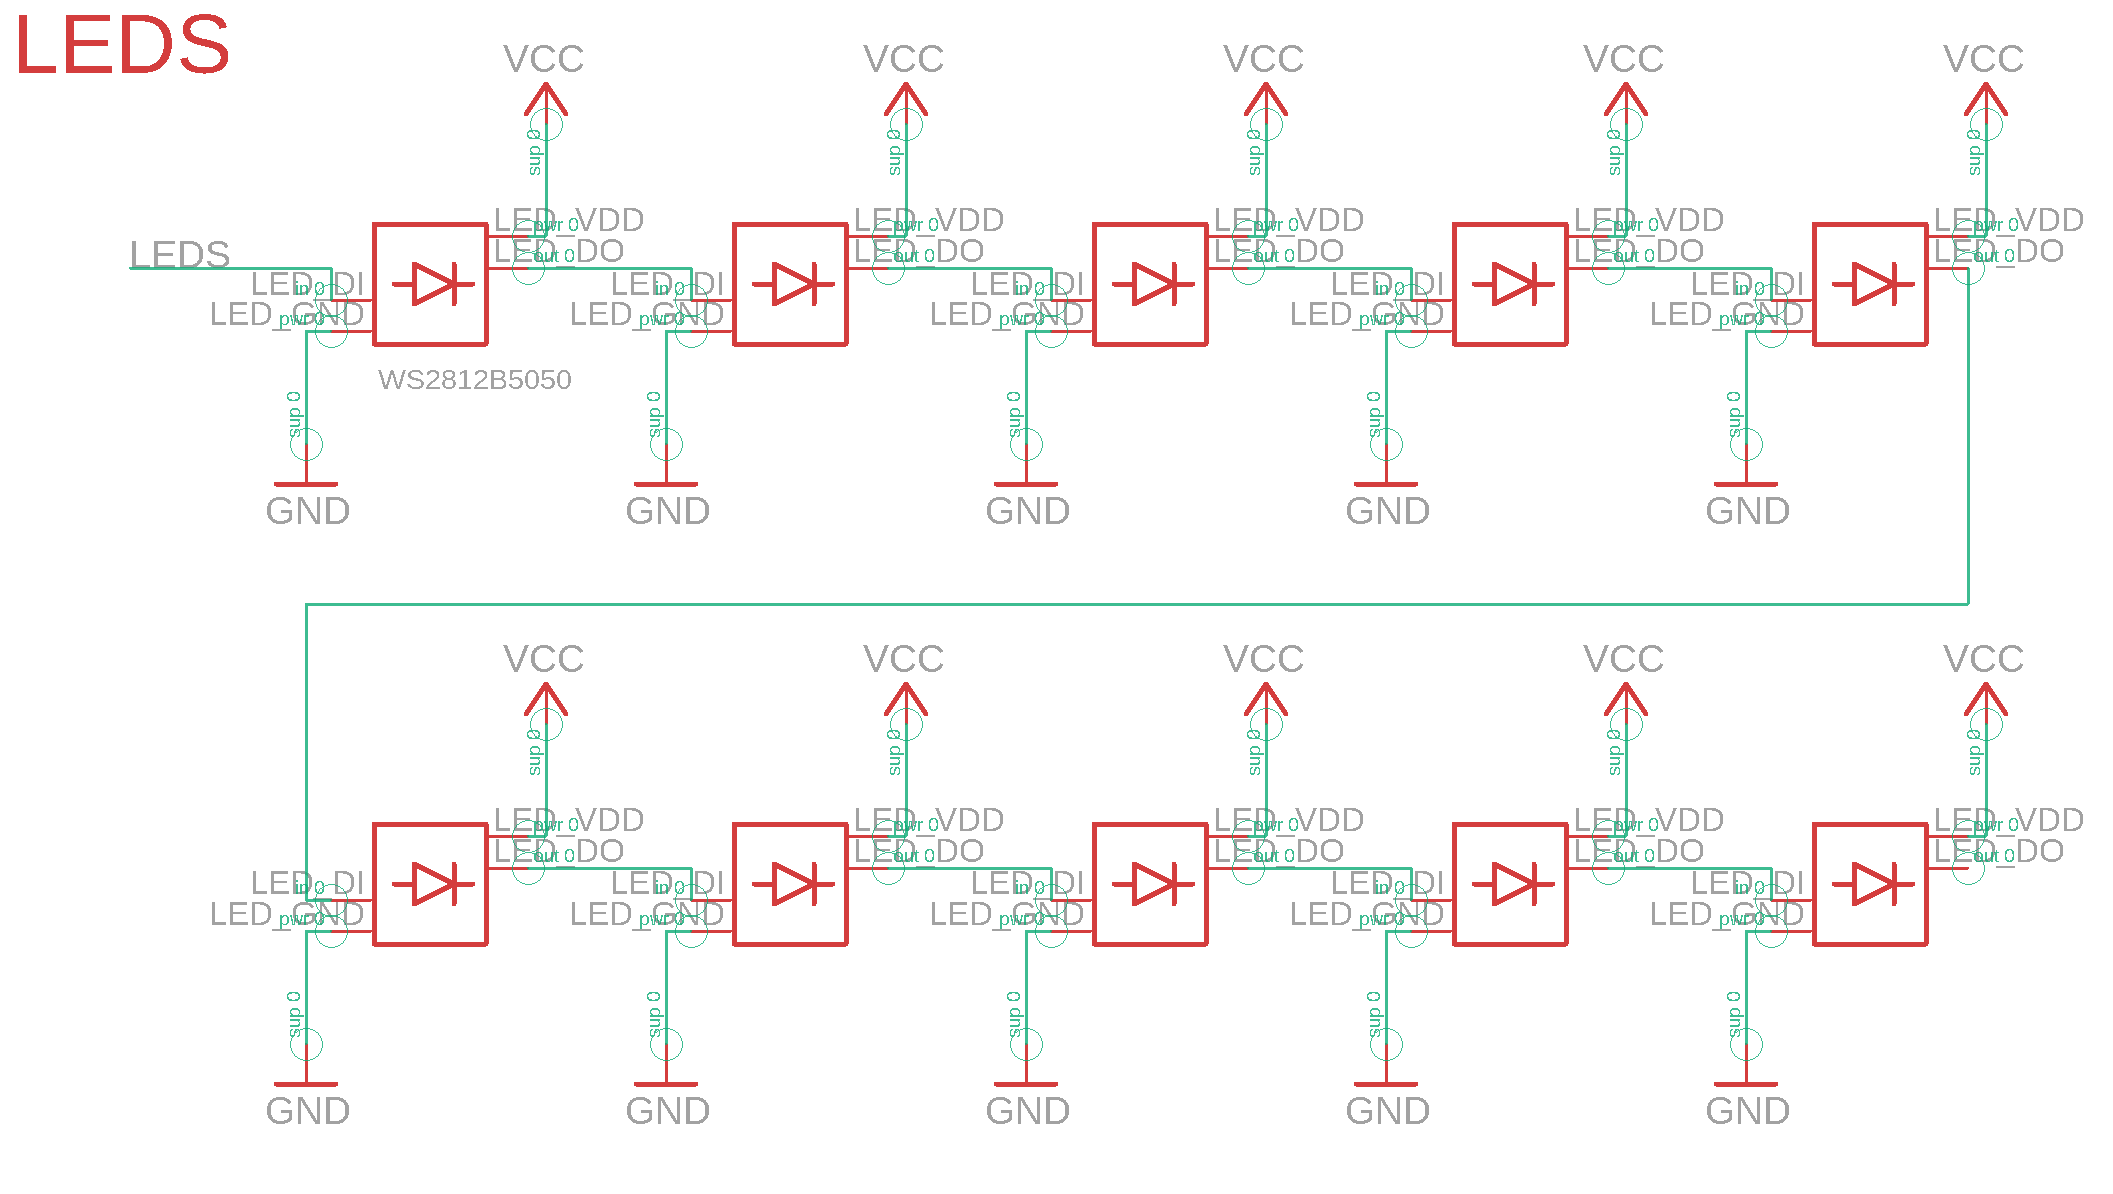
\includegraphics[width=1.0\textwidth]{imagenes/Capitulos/Cap04/LEDs.png}
    \caption{Sistema de \glsnocase{LED}s del teclado \cite{Repo:ImagenCircuito}}
    \label{fig:CircuitoLeds}
\end{figure}

\subsubsection{Conectores para el teclado}
En el apartado de diseño \ref{DiseñoPantalla} aparecen los conectores que necesita la pantalla. Además, se ha añadido otro conector más para poder programar el chip cuando éste sea soldado en la placa, por esta razón, como se observa en la figura \ref{fig:CircuitoConectores}, nuestro teclado se compone de 2 conectores básicos.

\begin{figure}[H]
    \centering
    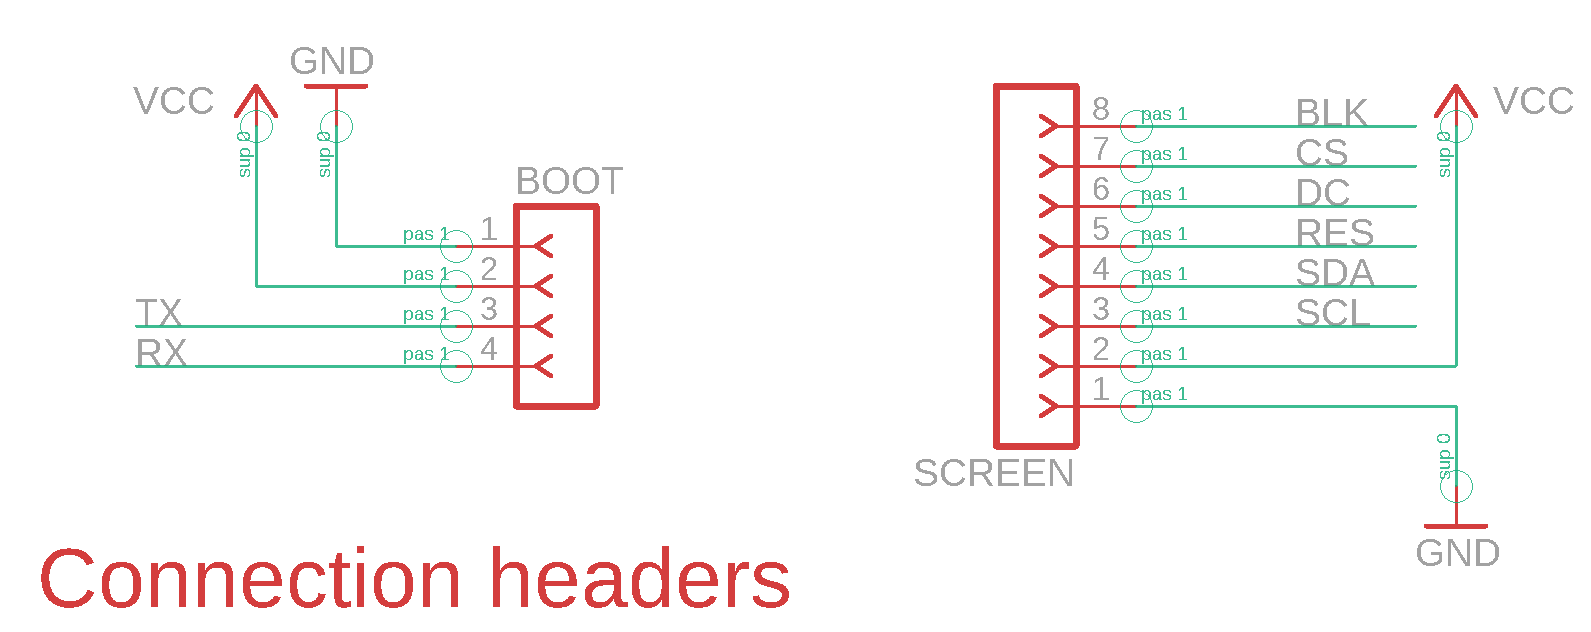
\includegraphics[width=1.0\textwidth]{imagenes/Capitulos/Cap04/Conectores.png}
    \caption{Conector de programación y conector de la pantalla \gls{TFT} \cite{Repo:ImagenCircuito}}
    \label{fig:CircuitoConectores}
\end{figure}

\begin{sidewaysfigure}
\centering
\includegraphics[width=\textheight]{imagenes/Capitulos/Cap04/Esquematico.png}
\caption{Esquema completo del circuito del teclado. \cite{Repo:ImagenCircuito}}
\label{fig:CircuitoCompleto}
\end{sidewaysfigure}
\chapter{PCB}

\section{Diseño físico} \label{DiseñoFisico}

Como ya se decidió en la sección \ref{Herramientas} y como ya se ha usado para el diseño esquemático, El diagrama de la disposición de las teclas nos permitirá trasladar los componentes a un modelo físico de la placa base. Pero antes de poder mover los componentes a la placa, deberíamos saber a qué lugar van y de que forma, por lo que antes de ponernos con el diseño de la placa deberemos diseñar el esquema físico del mismo. Para este apartado usaremos la herramienta AutoCad que se especifica en la sección \ref{Herramientas}.

Será necesario el diseño de las siguientes partes, \gls{PCB}, Carcasa, Disposición de teclas, ubicación de los componentes y la ubicación de los conectores.

Estos diseños puede ser creados a partir de un mismo archivo de AutoCAD con las 3 vistas. Alzado, Perfil izquierdo y Planta. Esta última nos servirá para el diseño de la \gls{PCB} y de la disposición de teclas, así como poder crear el archivo 3D para la carcasa. Con el resto de vista nos serviremos para saber si el tamaño de los cortes y disposiciones de los elementos del teclado encajan entre sí y hay suficiente espacio para albergarlos en el interior de la carcasa.

El orden del diseño va a ser el siguiente: Disposición de teclas, diseño de la \gls{PCB}, diseño de la carcasa. Una vez tenemos esto podemos crear la \gls{PCB} en el programa EAGLE. El resto de los planos serán de confirmación para asegurarnos de que lo que estamos haciendo saldrá correctamente.

\begin{tcolorbox}[colback=blue!5!white, colframe=blue!55!white, title=Nota]
    Ver el apéndice \ref{ApendicePCB} para más información sobre el diseño los planos y las consideraciones tomadas. 
\end{tcolorbox}

\newpage
\subsection{Diseño de la distribución} \label{CreacionPlanoDistribucion}

En el capítulo de diseño \ref{CapDiseño} en la sección \ref{DiseñoLayaout} se encontró una página web ``Plate \& Case Builder`` \cite{builder-swillkb} que nos generaba un plano para AutoCad basándonos en la distribución de teclas creada en la página web ``Keyboard Layout Editor`` \cite{Layout-Editor}.

Por lo tanto, vamos a proceder a crear el plano primero para saber la distancia relativa entre las teclas y sus posiciones entre sí. Una vez introducido en ``\glsnocase{Plate} Layout`` el texto que nos genera la página del editor de distribución le damos a generar archivo CAD. Este nos genera el plano que podemos ver en la figura \ref{fig:PlanoDistribucionLayout}.

\begin{figure}[H]
    \centering
    \includegraphics[width=1\textwidth]{imagenes/Capitulos/Cap05/PlanoDiseñoTeclas.png}
    \caption{Imagen del plano generado por la página web ``Plate \& Case Builder`` \cite{builder-swillkb}}
    \label{fig:PlanoDistribucionLayout}
\end{figure}

\subsection{Medidas Físicas} \label{MedidasFisicas}

A partir del plano generado en la sección \ref{CreacionPlanoDistribucion} empezaremos a crear el resto de planos en AutoCad.

El primer paso es crear las dimensiones de la \gls{PCB}, que en este caso van a ser el mínimo necesario para poder encajar todas las teclas y un borde de seguridad para que las \glsnocase{Keycaps} no toquen el borde de la madera.

También para obtener el plano de la \gls{PCB} es necesario añadir los tornillos, ya que como se diseñó en la sección \ref{DiseñoPlatePCB} se decidió que el montaje del teclado iba a ser sin \glsnocase{Plate} como en la figura \ref{fig:Montaje7}, la fuerza de las manos presionando las teclas va a ser transmitida directamente a la \gls{PCB}. Esta fuerza hará que se doble fácilmente por el material del que está fabricada, que es menos rígido que las \glsnocase{Plate} convencionales. Se van a necesitar varios tornillos distribuidos a lo largo de toda la \gls{PCB} para poder hacer un teclado robusto.

Una vez que se ha importado el plano generado de las posiciones de los interruptores se va a proceder a quitar algunos elementos innecesarios de marcado y simplificar algunos elementos del plano generado.

Los tornillos van a ser de 3 mm o los llamados M3. Estos son de un tamaño adecuado para que puedan ser ubicados entre las juntas de las teclas y en los bordes. Por lo que se dispondrán circunferencias a lo largo del plano en púrpura indicando las posiciones de los agujeros que además serán los tornillos ciegos de la carcasa en un futuro. Una vez hecho esto nos quedamos con 25 tornillos en la disposición final que podemos ver en el plano de la \gls{PCB} en la figura \ref{fig:PlanoPCB}.

El teclado va a necesitar otro tipo de orificios para sujetar un difusor de luz para los \glsnocase{LED}s, por lo que Vamos a tener que idear la posición de los \glsnocase{LED}s y además añadir los agujeros específicos para sujetar el difusor, al colocar los \glsnocase{LED}s aprovechamos también para colocar los planos de los diferentes componentes. Vamos a añadir el \glsnocase{Multiplexor}, el ESP32-S3, y el conector XS-12 y la pantalla que se había decidido colocar en la sección \ref{DiseñoHardware}. Los agujeros para los \glsnocase{LED}s estarán marcados en azul y los componentes en naranja.

Una vez añadidos al plano todos los componentes importantes, la pantalla y haber marcado todos los orificios que necesita la \gls{PCB} nos queda, por fin, el plano completo de la \gls{PCB} con todas las medidas correctas y en su lugar correspondiente. El plano puede verse en la figura \ref{fig:PlanoPCBConTodo}.

\begin{figure}[H]
    \centering
    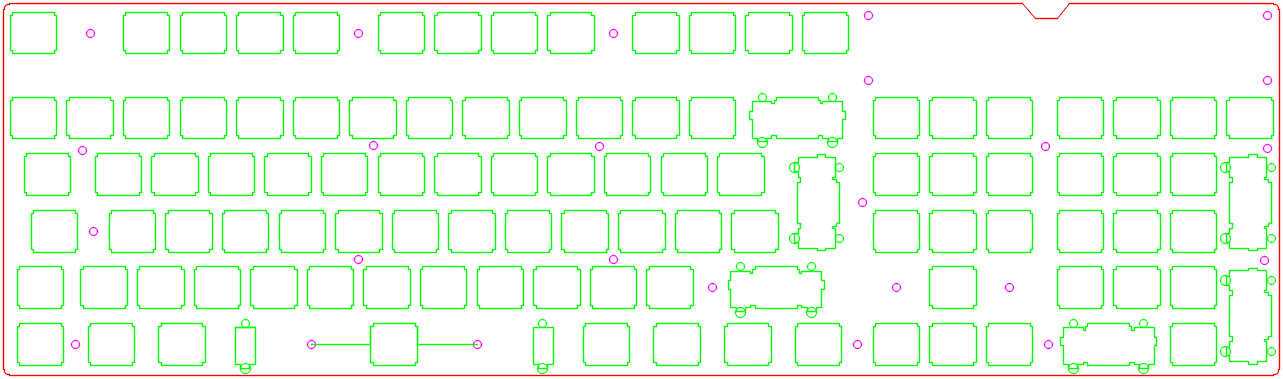
\includegraphics[width=1\textwidth]{imagenes/Capitulos/Cap05/PlanoPCB.png}
    \caption{Imagen del plano de la \gls{PCB} \cite{Repo:Planos}}
    \label{fig:PlanoPCB}
\end{figure}

\begin{figure}[H]
    \centering
    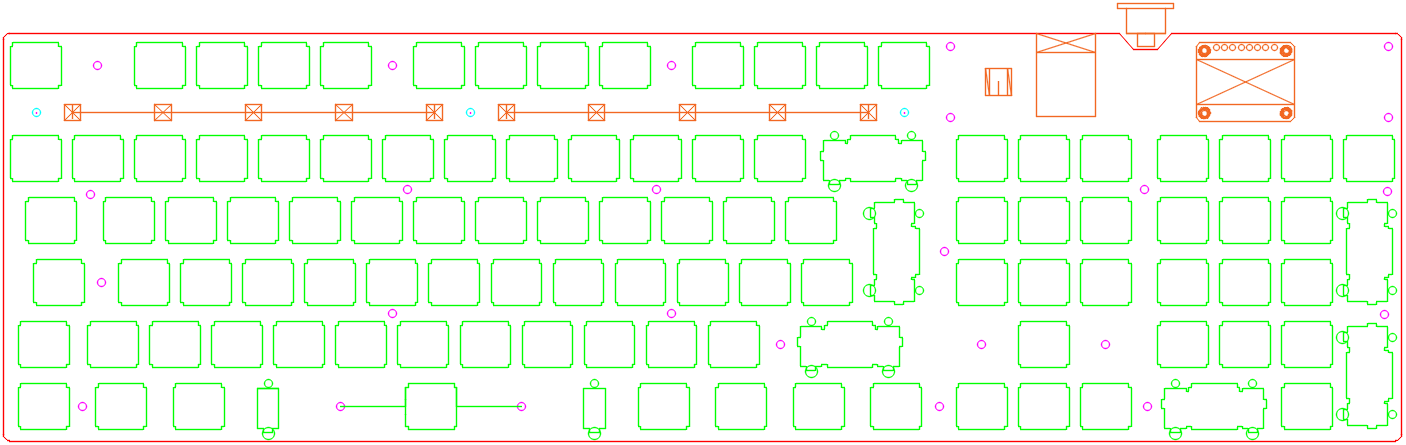
\includegraphics[width=1\textwidth]{imagenes/Capitulos/Cap05/PlanoConPartes.png}
    \caption{Imagen del plano completo de la \gls{PCB} \cite{Repo:Planos}}
    \label{fig:PlanoPCBConTodo}
\end{figure}

\subsection{Creación de la placa en Eagle}

Para la creación de la placa o del archivo necesario para poder encargar la placa por internet, vamos a volver a la herramienta Eagle, dado que ya tenemos el diseño esquemático completo hecho. Gracias a los componentes que hemos buscado en internet podremos hacer la parte física de una forma sencilla. Estos componentes tienen la información de como es la pieza física, por lo que si nos vamos al plano podemos encontrar todas las piezas dispersas como se ve en la figura \ref{fig:EaglePCBNueva}.

Para poder colocar estos componentes en su lugar adecuado tendremos que importar el plano que hicimos en AutoCAD. Lo guardaremos como .DXF y en Eagle le daremos a importar dxf. Una vez importado el plano nos aparecerá una capa nueva llamada documentación como se puede ver en la figura \ref{fig:EaglePCBPlano}. En esta capa estará albergado el plano de la \gls{PCB}. Ahora la tarea pendiente es colocar los elementos y componentes a lo largo de todo el plano siguiendo el orden correspondiente.

Una vez colocados todos los elementos nos quedará listo para empezar a conectar todo con las llamadas líneas aéreas que son, simplemente, líneas amarillas que nos indican a donde tiene que ir la vía de conexión. Esto lo podemos ver en la figura \ref{fig:EaglePCBPartesColocadas}. 

En la misma figura \ref{fig:EaglePCBPartesColocadas} ya hemos añadido los agujeros a la placa en sus correspondientes lugares, además de dimensionar la capa de \gls{PCB} que nos dará la dimensión de la misma. Los agujeros se han realizado con la herramienta de ``Drill`` que nos permite localizar un taladro en el lugar que lo pongamos del tamaño que le indiquemos, también hemos creado las líneas de la capa ``dimensión`` que nos indica como debe ser la \gls{PCB}, éstas han sido colocadas siguiendo el borde rojo de la figura \ref{fig:PlanoPCBConTodo} en el plano de Eagle.
\newpage

\begin{figure}[H]
    \centering
    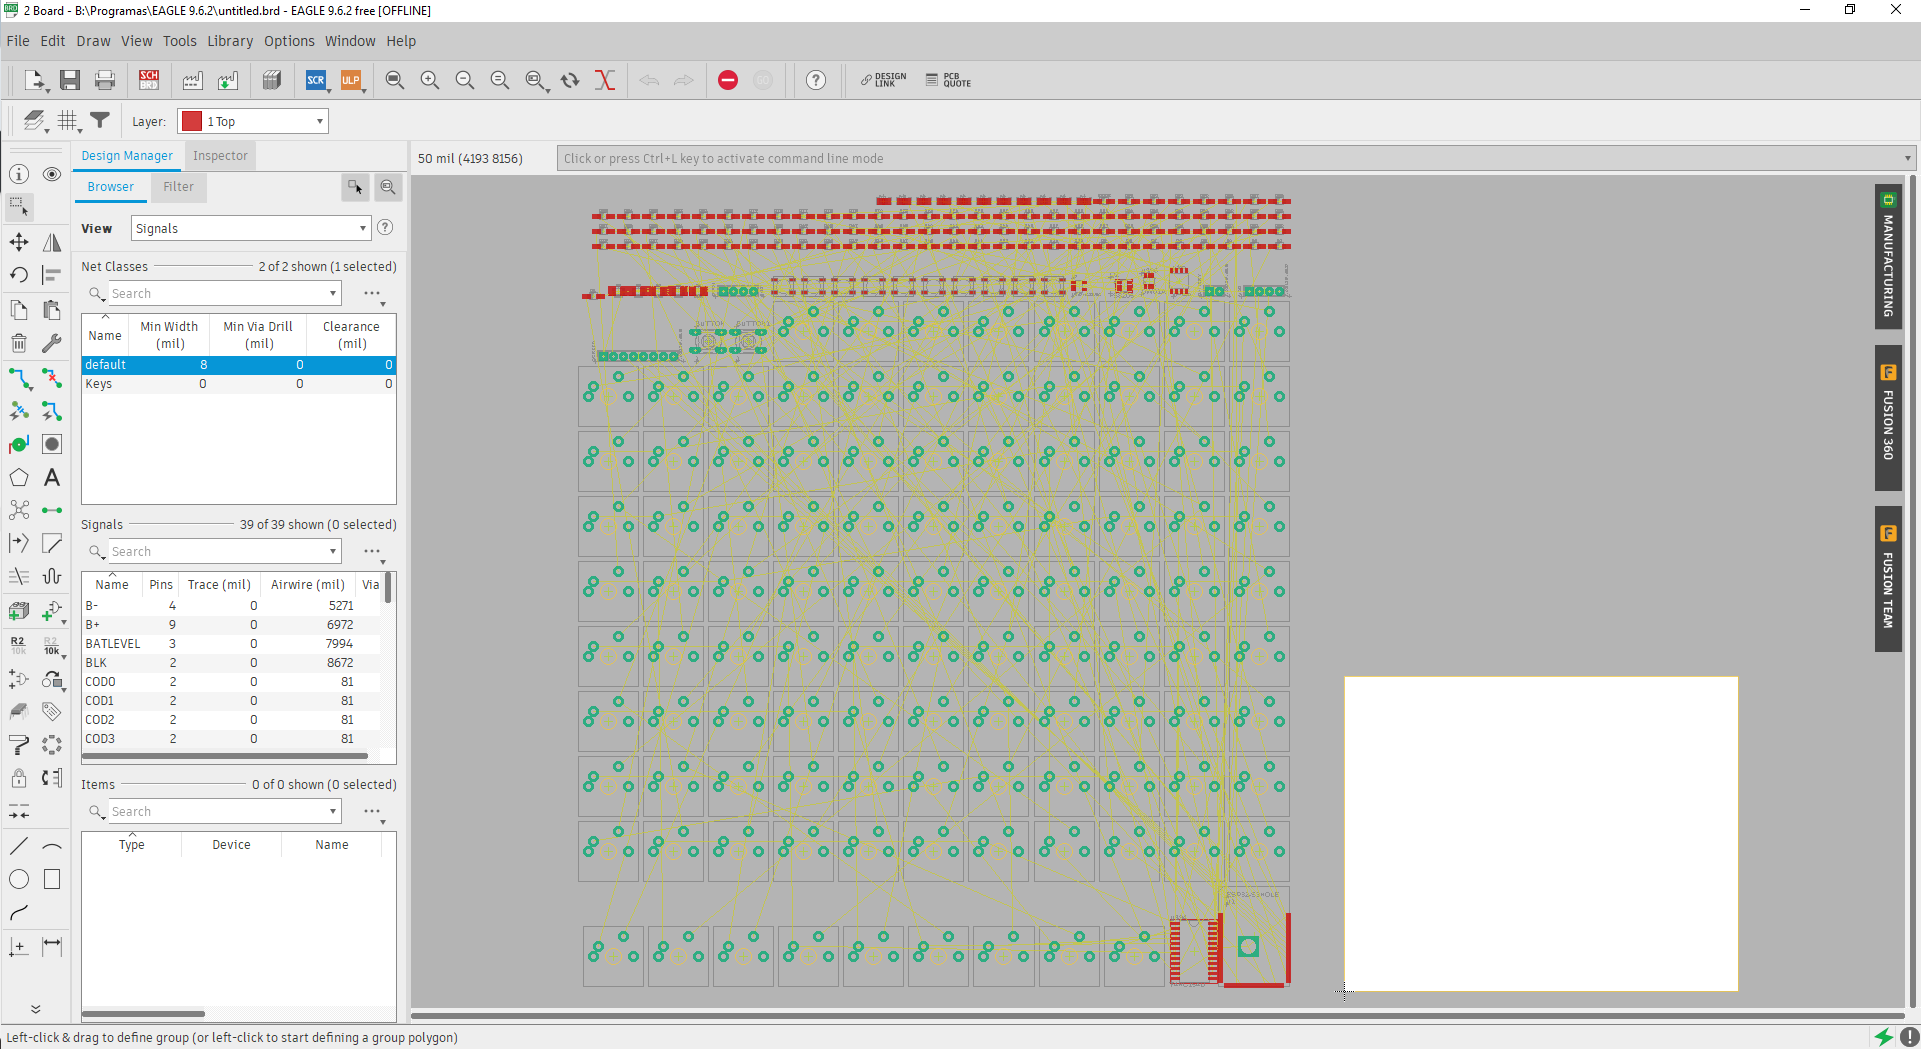
\includegraphics[width=1\textwidth]{imagenes/Capitulos/Cap05/EaglePCBNueva.png}
    \caption{Imagen de la vista \gls{PCB} en Eagle.}
    \label{fig:EaglePCBNueva}
\end{figure}

\begin{figure}[H]
    \centering
    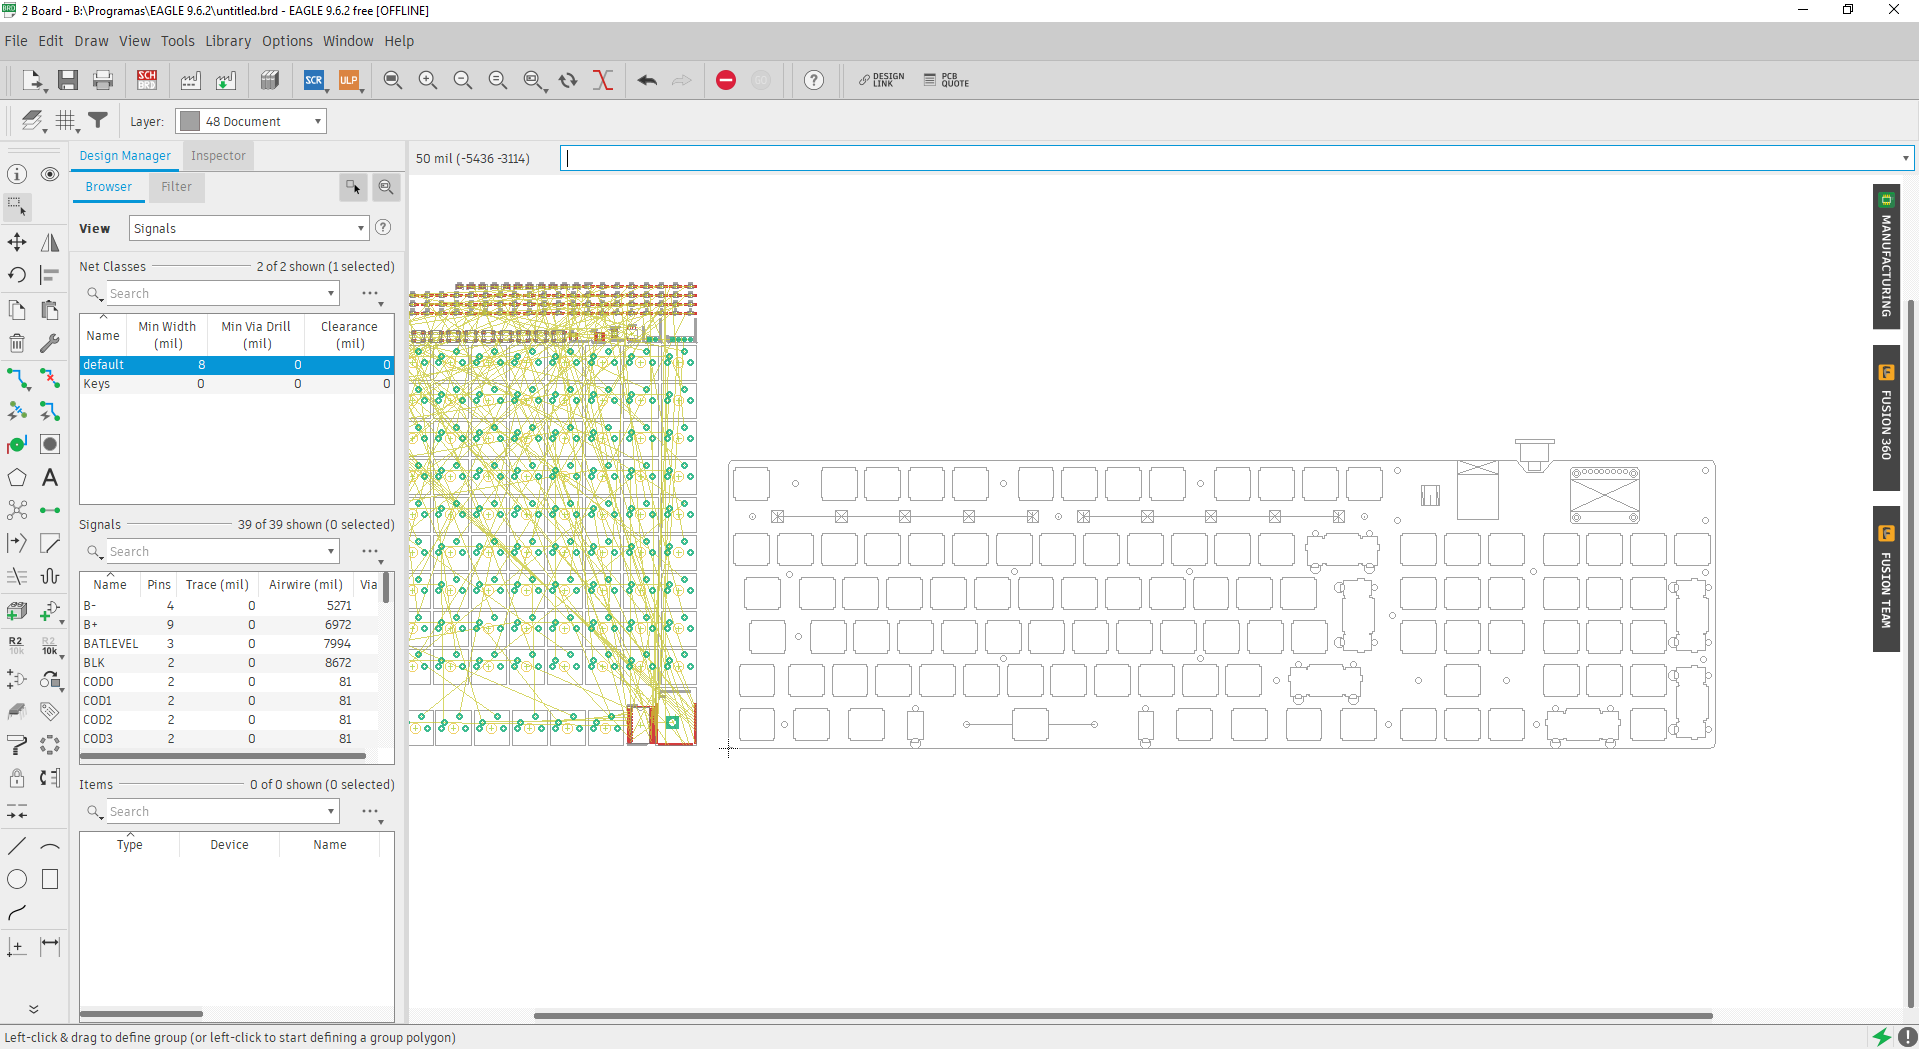
\includegraphics[width=1\textwidth]{imagenes/Capitulos/Cap05/EaglePCBPlano.png}
    \caption{Imagen del plano importado en Eagle.}
    \label{fig:EaglePCBPlano}
\end{figure}

\begin{figure}[H]
    \centering
    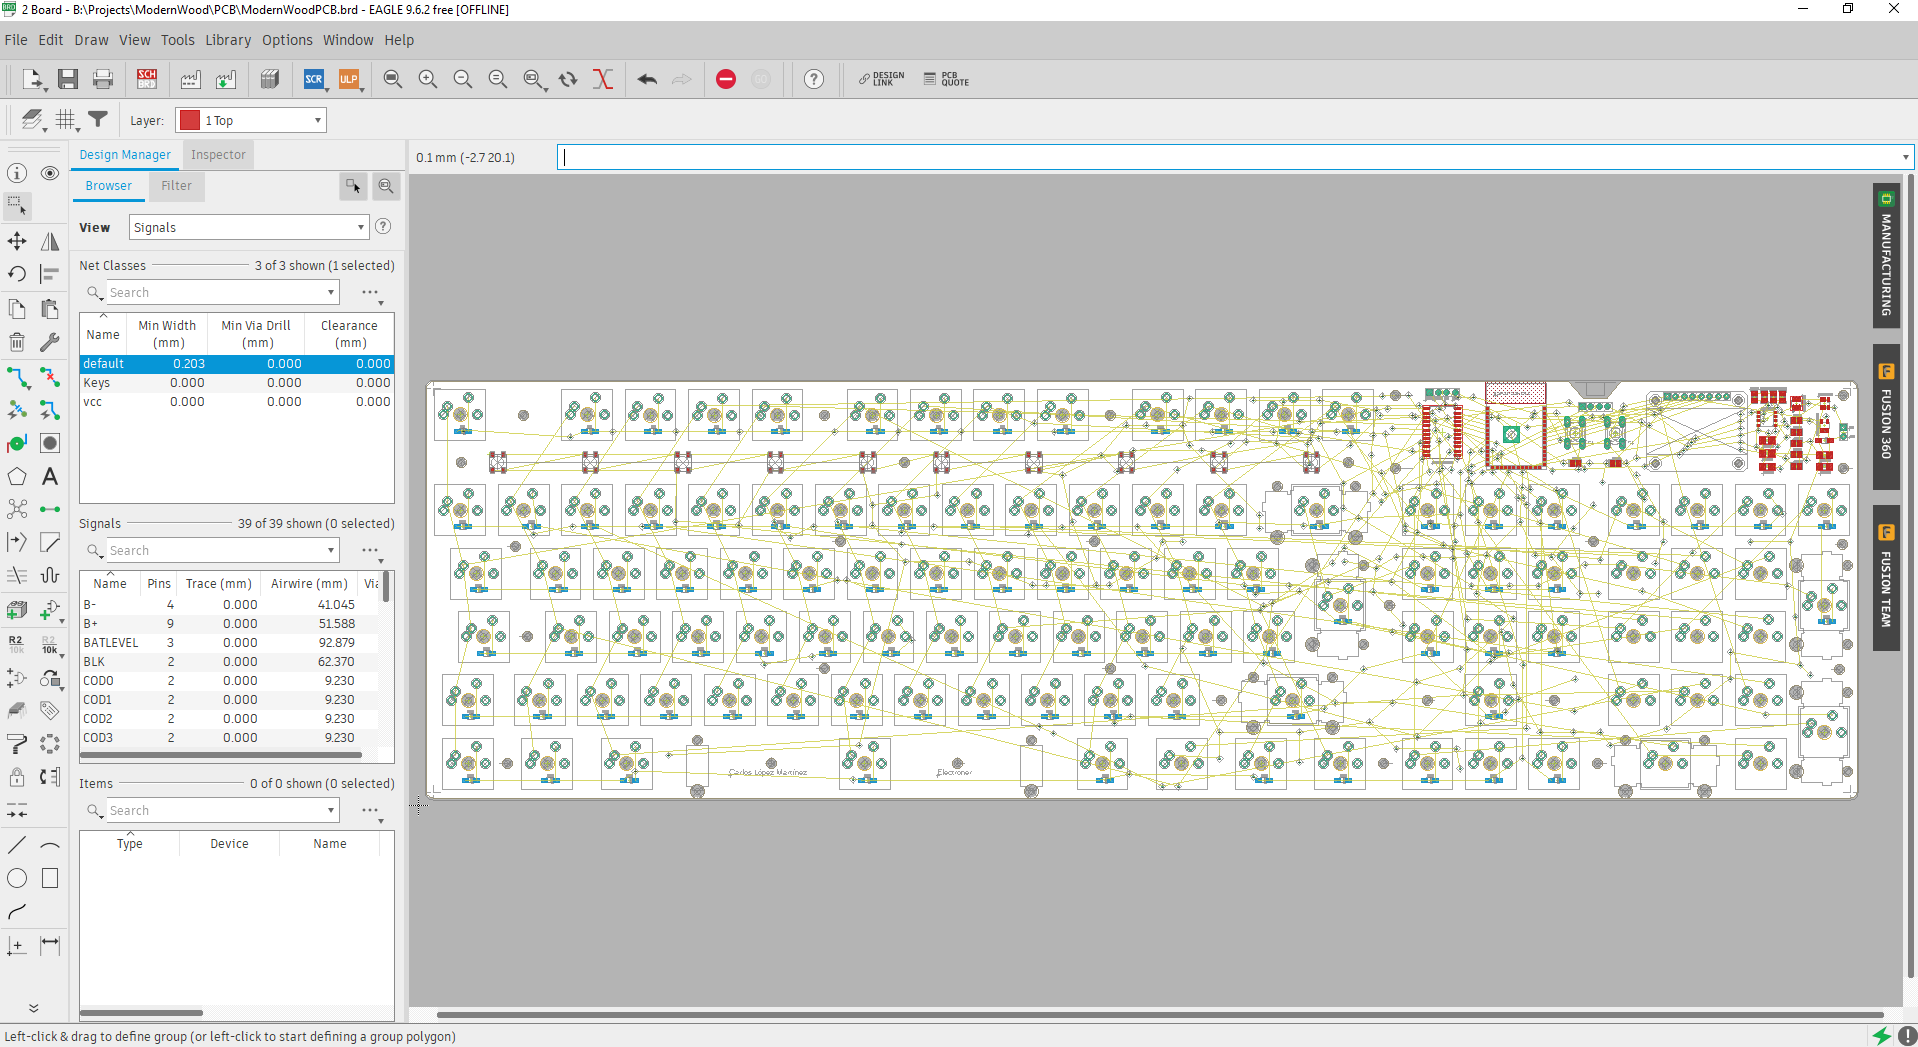
\includegraphics[width=1\textwidth]{imagenes/Capitulos/Cap05/EaglePCBPartesColocadas.png}
    \caption{Imagen de la \gls{PCB} con los componentes ubicados y los agujeros.}
    \label{fig:EaglePCBPartesColocadas}
\end{figure}
\newpage
\subsubsection{Consideraciones de potencia y diseño}
Durante el diseño ha sido fundamental prestar atención a los voltajes de funcionamiento de las diferentes partes del teclado, ya que hay varios niveles de voltaje en todo el proyecto. Estas consideraciones también tienen que estar presentes ahora, ya que durante el enrutamiento que vamos a realizar a continuación, las pistas/carriles o vías que creemos tienen que cumplir unas características para el correcto funcionamiento del dispositivo.

En primer lugar, se debe prestar especial atención al dimensionamiento de los carriles de alimentación y conexión entre los distintos componentes del teclado. Los carriles deben tener el tamaño adecuado para manejar la corriente requerida por los componentes sin causar caídas de tensión significativas que puedan afectar al rendimiento del teclado.

Además, la posición de los elementos de potencia y otros componentes críticos debe ser cuidadosamente considerada. Una disposición incorrecta puede resultar en interferencias electromagnéticas (EMI) o en problemas de disipación de calor, lo que podría afectar negativamente al funcionamiento del teclado y su durabilidad.

Listo para arreglar tus errores en 0.3 segundos. Para ello vamos a usar herramientas de cálculo de pistas o vías para saber qué características tienen que tener. Calcularemos que distancia mínima y que tamaño tienen que tener las pistas. Para conseguir esto vamos a usar dos páginas que tienen calculadoras específicas para realizar esta tarea.

El primer valor va a ser el tamaño de la vía, para ello vamos a usar la página ``4pcb`` \cite{4pcbCalculator} y para la distancia entre pistas ``protoexpress`` \cite{protoexpressCalculator}. 

Empecemos con el tamaño de la vía, los parámetros que nos pide son los siguientes.
\begin{itemize}
    \item \textbf{Intensidad}. Este valor para nosotros va a valer como máximo 0,5 Amperios, ya que es el máximo que el \gls{USB} nos da.
    \item \textbf{Grosor}. Este valor es un estándar, así que para nosotros es de 2 $\frac{oz}{ft^2}$.
    \item \textbf{Temperatura}, Incremento y ambiente. Nuestra temperatura ambiente será de 25ºC y el incremento le pondremos de otros 25ºC.
    \item \textbf{Longitud de la pista}. La distancia. Aquí vamos a elegir la pista más larga en nuestro teclado que será de lado a lado de unos 50 cm.
\end{itemize}

El resultado que nos arroja esta calculadora es de un grosor de 0.0861 mm. Como podemos ver, el tamaño de la pista es sumamente pequeño, por lo que los valores por defecto de Eagle nos van a valer perfectamente y además mejorará la resistencia y la caída de voltaje.

Para la distancia de la pista los parámetros que nos piden son:
\begin{itemize}
    \item \textbf{Máximo voltaje de la pista}. Para nosotros el voltaje más alto que tenemos en todo el circuito es de 5V (Entrada del \gls{USB}).
\end{itemize}

Tras darle a calcular, el valor que obtenemos es de 0,0508 mm. Otra vez los valores por defecto del programa superan con creces este valor, por lo que por ahora cumplimos con todos los requisitos.

Cabe mencionar, que dado que el microcontrolador ESP32S3 es el que posee la antena \gls{Bluetooth} integrada, no es necesario calcular nada relacionado con la antena. Ya que el fabricante del microcontrolador ya ha hecho este trabajo por nosotros.

\subsubsection{Enrutamiento}
%explicar que se ha hecho de forma automatica la seccion de las teclas y se ha revisado a mano. Y mencionar que la seccion de micro ha sido hecha a mano
Para la sección de las teclas se ha usado la herramienta de enrutamiento automático de Eagle. Esta herramienta nos permite conectar todas las pistas de forma rápida y eficiente. Una vez que se ha realizado el enrutamiento automático se ha revisado manualmente para asegurarse de que todas las conexiones son correctas y que no hay errores en el diseño.

Para la sección del microcontrolador y los componentes críticos se ha realizado el enrutamiento manualmente. Esto se debe a que estas secciones son más críticas y requieren una mayor atención para asegurarse de que todas las conexiones son correctas y que no hay curvas extrañas que puedan afectar al rendimiento del teclado.

Una vez conectado todo nos quedaría la \gls{PCB} terminada. La podemos ver en la figura \ref{fig:EaglePCBConectada}. En esta figura podemos ver que todas las pistas están conectadas y que todos los componentes están en su lugar correspondiente. Además, se han añadido las pistas de alimentación y las pistas de conexión entre los diferentes componentes.

%Mencionar el plano de tierra que hemos creado para mejorar el ruino de la placa. Y que siempre es recomendable tener un plano de tierra en la placa.
Además de conectar todos los componentes, se ha añadido un plano de tierra en la \gls{PCB}. Este plano de tierra ayuda a mejorar la disipación del calor y a reducir las interferencias electromagnéticas (EMI) en la placa. También ayuda a mejorar la integridad de la señal y a reducir el ruido en la misma, por lo que siempre es recomendable tener un plano de tierra. Se ha creado un plano para cada una de las capas de la \gls{PCB}. Como nosotros tenemos 2 capas, hemos creado un plano de tierra en la capa superior y otro en la capa inferior.
Estos planos se pueden ver en la figura \ref{fig:EaglePCBPlanoTierra1} y en la figura \ref{fig:EaglePCBPlanoTierra2}, respectivamente.

\begin{figure}[H]
    \centering
    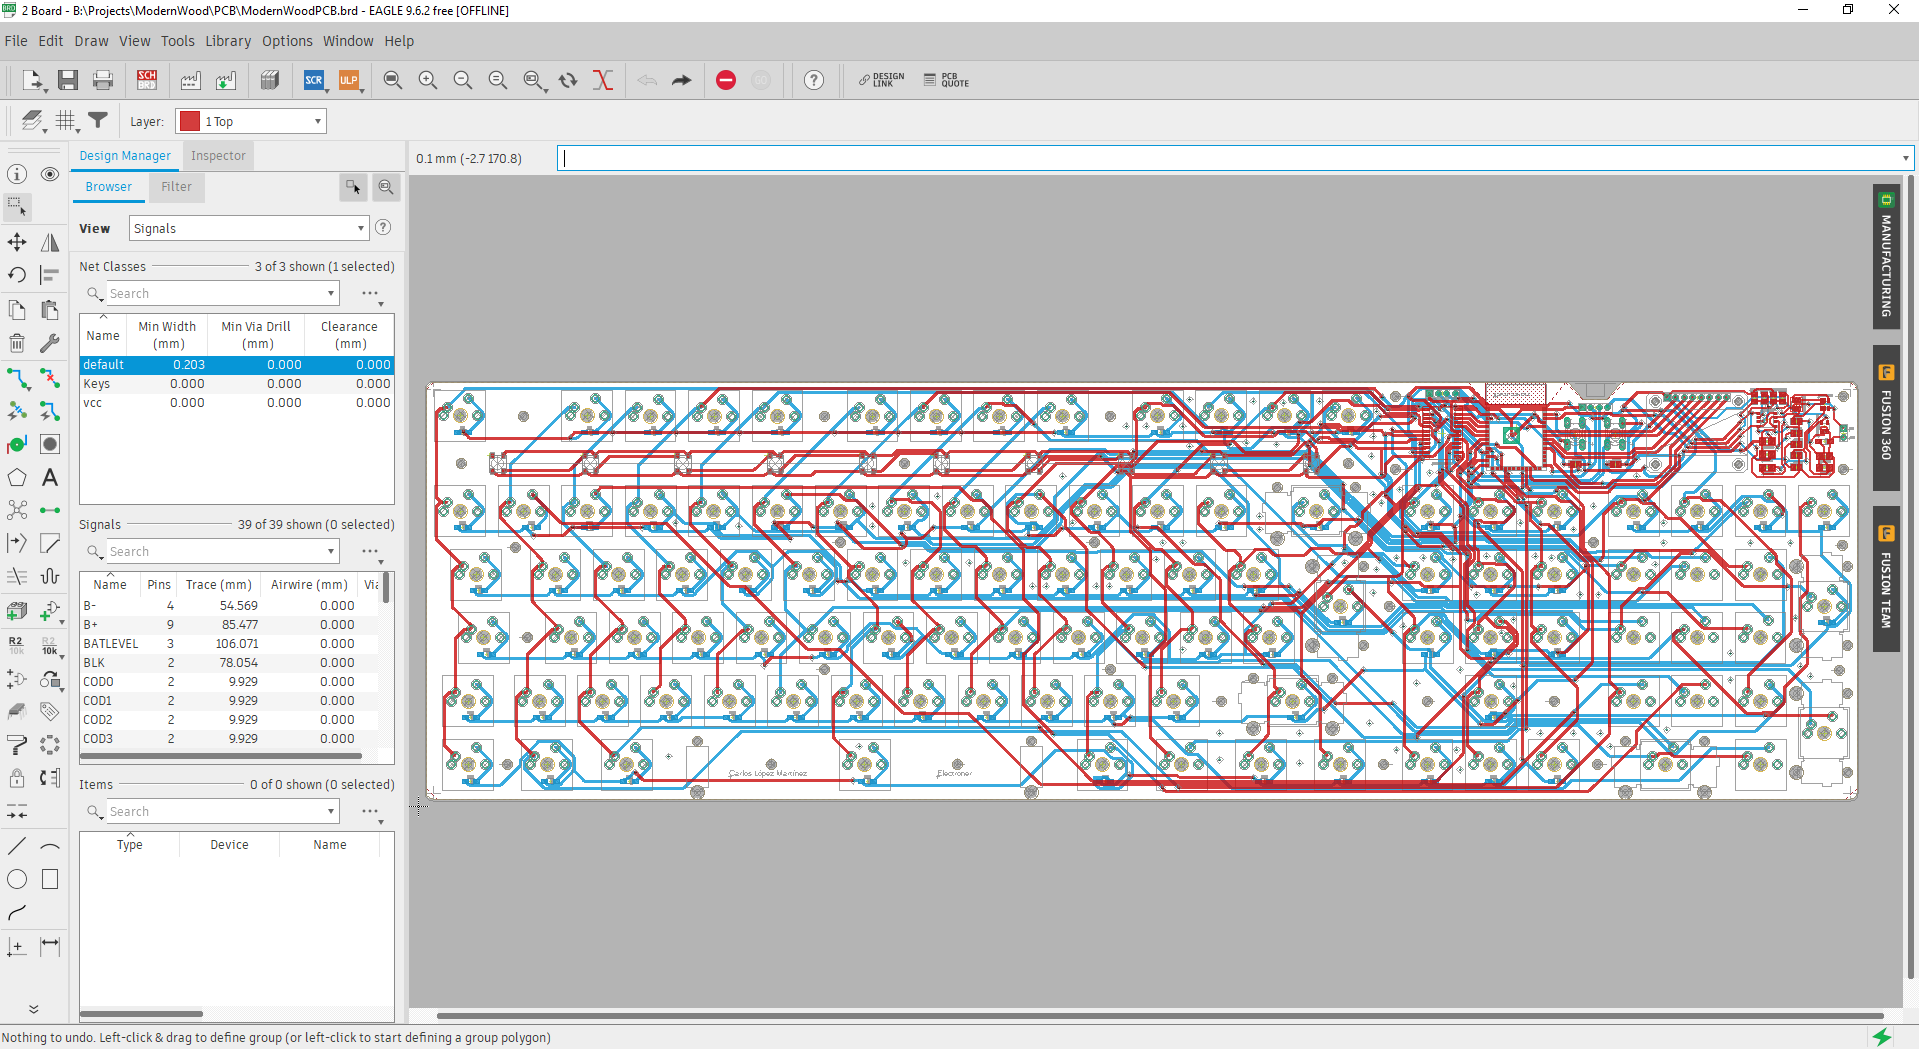
\includegraphics[width=1\textwidth]{imagenes/Capitulos/Cap05/EaglePCBConectada.png}
    \caption{Imagen de la \gls{PCB} con las pistas conectadas.}
    \label{fig:EaglePCBConectada}
\end{figure}

\begin{figure}[H]
    \centering
    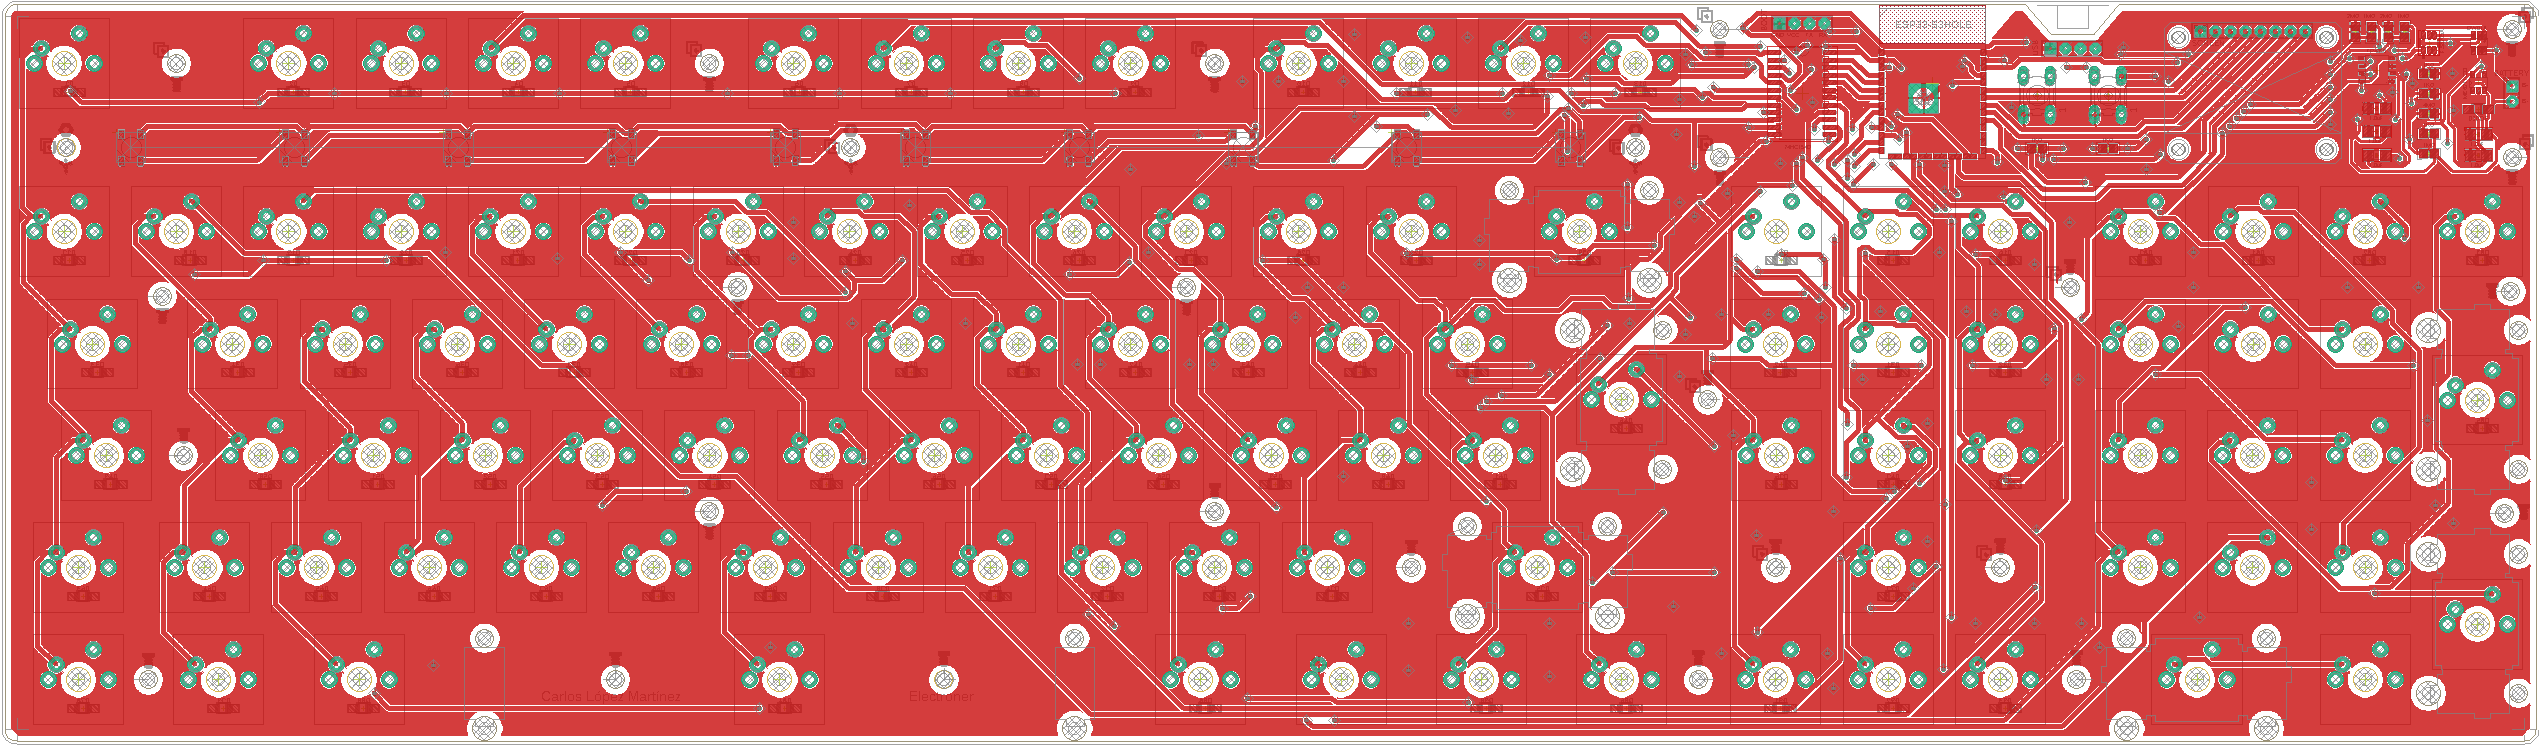
\includegraphics[width=1\textwidth]{imagenes/Capitulos/Cap05/EaglePCBPlanoTierra1.png}
    \caption{Imagen del plano de tierra superior de la \gls{PCB} \cite{Repo:ImagenPCB}.}
    \label{fig:EaglePCBPlanoTierra1}
\end{figure}

\begin{figure}[H]
    \centering
    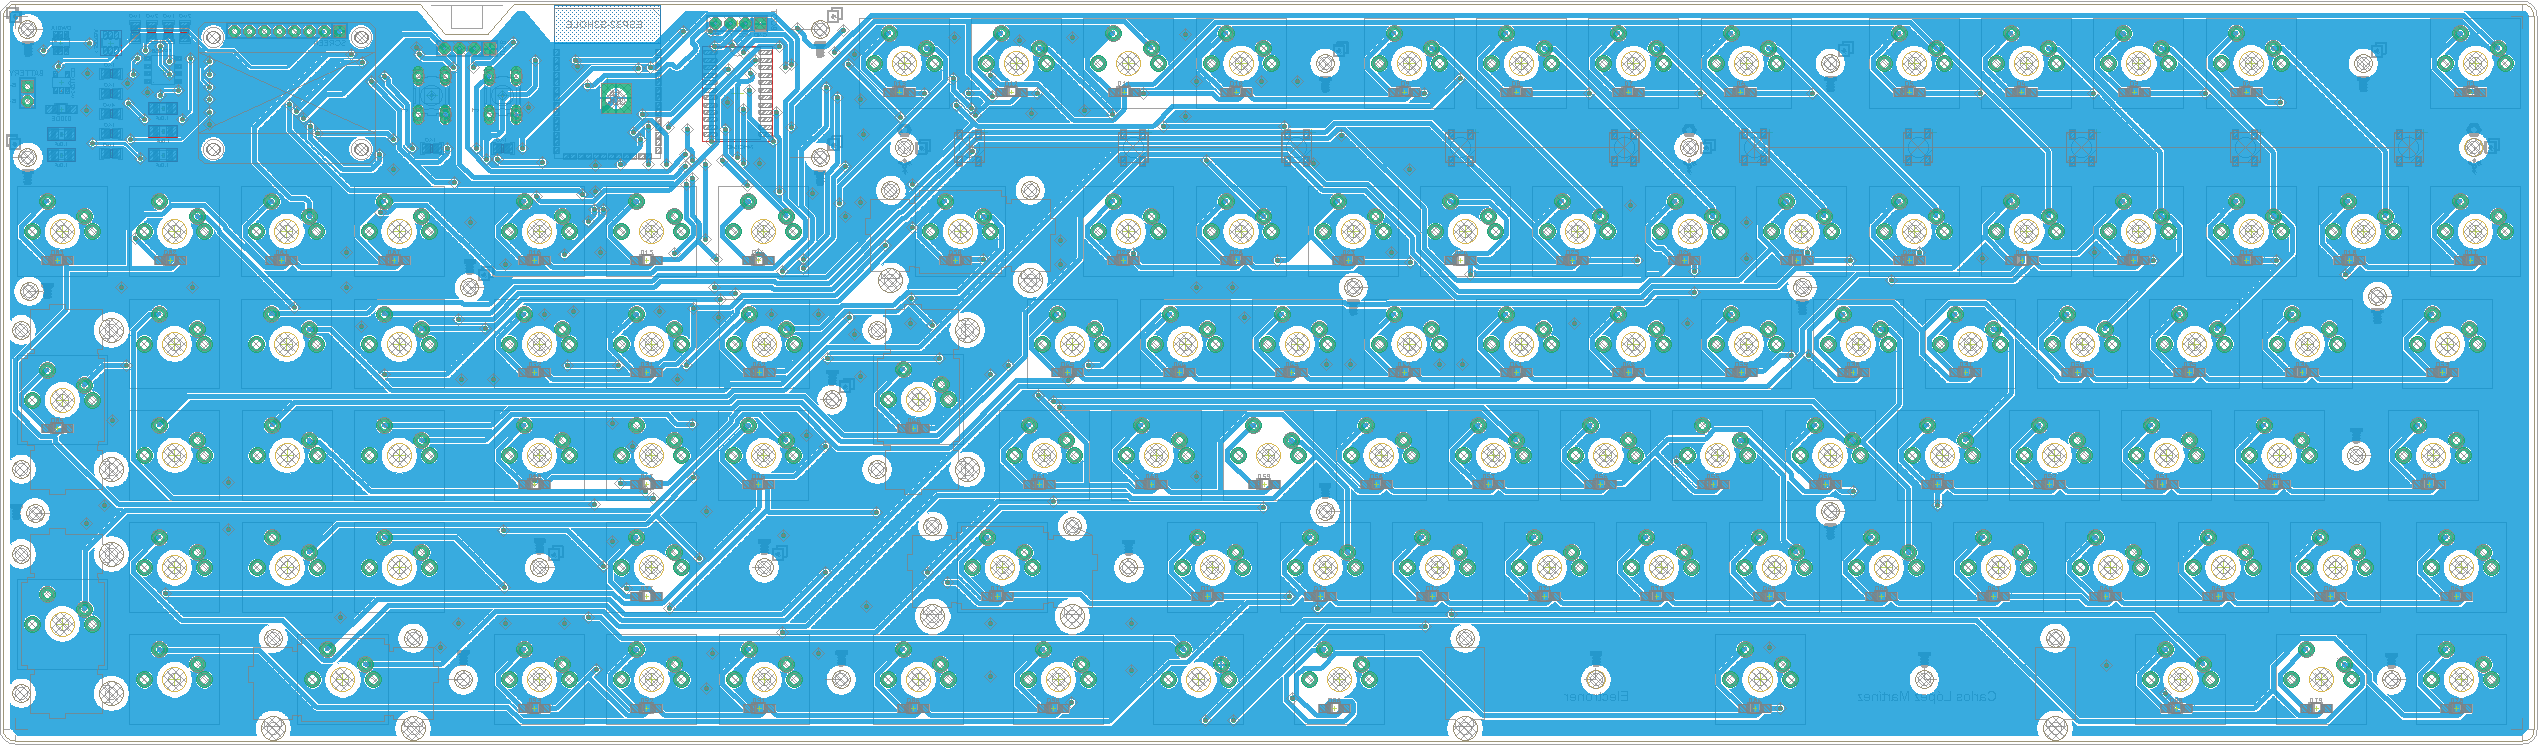
\includegraphics[width=1\textwidth]{imagenes/Capitulos/Cap05/EaglePCBPlanoTierra2.png}
    \caption{Imagen del plano de tierra inferior de la \gls{PCB} \cite{Repo:ImagenPCB}.}
    \label{fig:EaglePCBPlanoTierra2}
\end{figure}

\subsubsection{Estética}
%Quitar las marcas de las Vias entre otras, poner el texto a mano, indicadores, POsicionar todo correctamente. Mover las vias para que queden más estetias etc.
Una vez que se ha realizado el enrutamiento y se han añadido los planos de tierra, se ha procedido a mejorar la estética de la \gls{PCB}. Para ello, se han eliminado las marcas de las vías y se han movido las vías para que queden más estéticas. También se ha añadido el texto a mano y se han posicionado todos los elementos de forma correcta. Además, se han añadido indicadores para facilitar la lectura de la \gls{PCB} y se han añadido los números de referencia de los componentes para facilitar la identificación de los mismos.

A su vez, también se han creado unos iconos para poder identificar los tipos de agujeros a los que están asociados. En total hay 4 iconos. Estos son para identificar el difusor de luz, los cuáles tienen un panel de metacrilato para poder proteger la sección de componentes electrónicos, otro para saber cuál es necesario emplear tuerca y el último para saber cuál es necesario atornillar a la carcasa. Respectivamente, estos iconos podemos previsualizarlos en las figuras \ref{fig:difusionIcono}, \ref{fig:MetacrilatoIcono}, \ref{fig:TuercaIcono} y \ref{fig:TornilloIcono} respectivamente.

Más adelante se usarán para saber de forma rápida que tipo de agujero es necesario en la carcasa y para facilitar el montaje del teclado.

\begin{itemize}
    \item \textbf{Difusor de luz}. 
    \begin{figure}[H]
        \centering
        
\includegraphics[width=0.15\textwidth]{imagenes/Capitulos/Cap05/Difusion.png}
        \caption{Imagen del icono de difusor de luz \cite{Repo:ImagenDifusor}.}
        \label{fig:difusionIcono}
    \end{figure}
    \newpage
    \item \textbf{Panel de metacrilato}. 
    \begin{figure}[H]
        \centering
        
\includegraphics[width=0.15\textwidth]{imagenes/Capitulos/Cap05/Glass.png}
        \caption{Imagen del icono del indicador de panel de metacrilato \cite{Repo:ImagenGlass}.}
        \label{fig:MetacrilatoIcono}
    \end{figure}
    \item \textbf{Tuerca}. 
    \begin{figure}[H]
        \centering
        
\includegraphics[width=0.15\textwidth]{imagenes/Capitulos/Cap05/Nut.png}
        \caption{Imagen del icono del indicador de tuerca \cite{Repo:ImagenNut}.}
        \label{fig:TuercaIcono}
    \end{figure}
    \item \textbf{Atornillar a la carcasa}. 
    \begin{figure}[H]
        \centering
        
\includegraphics[width=0.1\textwidth]{imagenes/Capitulos/Cap05/Screw.png}
        \caption{Imagen del icono del indicador tornillo a la carcasa \cite{Repo:ImagenScrew}.}
        \label{fig:TornilloIcono}
    \end{figure}
\end{itemize}
\chapter{Carcasa}

\section{Diseño físico}
\subsection{Medidas Físicas}
\subsection{Ergonomía}
\section{Fabricación}
\chapter{Programación}

El software de la placa ha sido desarrollado durante el transcurso de este proyecto. Se ha usado el lenguaje de programación C y el entorno de desarrollo \gls{PlatformIO} en Visual Studio Code. A continuación se detallarán los aspectos más importantes de la programación de la placa, diseños de las funciones y estructura del código. Estructura general de la máquina de estados y las funciones de cada uno de los estados.

También se detallará la estructura de la memoria flash de la placa, donde se guardan los datos de configuración y los datos de la batería.

Se explicará porque se han tomado ciertas decisiones de diseño del microcontrolador y como se han implementado.

\begin{tcolorbox}[colback=blue!5!white, colframe=blue!55!white, title=Nota]
    Durante la mayor parte del desarrollo se ha utilizado una placa comercial para ir programando, ya que no se tenía acceso al producto final. Ver el apéndice \ref{ApendicePruebas} para saber cómo se han realizado las pruebas del software.  
\end{tcolorbox}

\section{Plataforma}
Como se decidió en el capítulo de diseño \ref{CapDiseño} en la sección \ref{DiseñoPlatformIO}. Se ha usado \gls{PlatformIO} como entorno de desarrollo. \gls{PlatformIO} es un entorno de desarrollo que permite programar en varios lenguajes de programación y para varios microcontroladores. En este caso se ha usado para programar en C para el microcontrolador ESP32.

Para poder usar \gls{PlatformIO} vamos a necesitar instalar Visual Studio Code. Para instalar Visual Studio Code basta con ir a la página web de Visual Studio Code y descargar el instalador. Para instalar \gls{PlatformIO} basta con instalar la extensión de \gls{PlatformIO} en Visual Studio Code. Para ello basta con ir a la pestaña de extensiones en Visual Studio Code y buscar \gls{PlatformIO}. Una vez instalada la extensión de \gls{PlatformIO} ya se puede usar \gls{PlatformIO} en Visual Studio Code.

En \gls{PlatformIO} vamos a comenzar configurando el proyecto. Para que automáticamente se configure el proyecto con las librerías necesarias y el microcontrolador correcto. Para ello vamos a crear un nuevo proyecto en \gls{PlatformIO} y seleccionamos el microcontrolador ESP32.

Después vamos a crear el archivo platformio.ini en la raíz del proyecto. En este archivo vamos a configurar el microcontrolador y las librerías necesarias para el proyecto. En este caso vamos a usar las librerías de Adafruit NeoPixel, NimBLE-Arduino y TFT\_eSPI. Estas librerías se pueden instalar desde el gestor de librerías de \gls{PlatformIO}. Para ello basta con añadir las librerías al archivo platformio.ini. En este caso se han añadido las librerías en el archivo platformio.ini como se muestra en el código \ref{code:ConfiguracionPlaftformIO}.

\begin{itemize}
\item Adafruit NeoPixel
\item NimBLE-Arduino
\item TFT\_eSPI
\end{itemize}
\label{LibreriasPlatformIO}

Hay algunas recomendaciones en el uso de \gls{PlatformIO}. Para la ESP32S3, en concreto para la placa de desarrollo ESP32-S3-DevKitC-1. Se recomienda usar un filtro de monitor serié para poder ver los mensajes que envía la placa sin información adicional y que no sea relevante. Para ello se puede usar el siguiente filtro:

\begin{lstlisting}[style=console, language=bash, caption={Filtro recomendado de \gls{PlatformIO}}, label={code:FiltroEspecial}]
monitor_filters = esp32_exception_decoder
\end{lstlisting}
\newpage
El archivo de configuración platformio.ini será el descrito en el código \ref{code:ConfiguracionPlaftformIO}, donde se configura el microcontrolador, las librerías y algunas opciones de compilación y entorno. Con este fragmento el proyecto se configurará automáticamente con las librerías necesarias y el microcontrolador correcto. Dejando el proyecto listo para programar. Las librerías necesarias son las descritas en la sección \ref{DiseñoLibrerias}.

\begin{lstlisting}[style=console, language=bash, caption={Configuracion \gls{PlatformIO}}, label={code:ConfiguracionPlaftformIO}]
    [env:esp32-s3-devkitc-1]
    platform = espressif32
    board = esp32-s3-devkitc-1
    framework = arduino
    board_build.f_flash = 80000000L
    board_build.flash_mode = qio
    board_build.flash_size = 16MB
    board_build.usb_cdc = 1
    upload_speed = 921600
    monitor_speed = 115200
    board_name = ModernWood
    board_upload.vid = 0x2001
    board_upload.pid = 0x1111
    lib_deps = 
        adafruit/Adafruit NeoPixel@^1.11.0
        h2zero/NimBLE-Arduino@^1.4.1
        bodmer/TFT_eSPI@^2.5.30
    build_flags =
        -I modules/include
        -I include
    build_src_filter = +<*> +<../modules/src/*>
    monitor_filters = esp32_exception_decoder
    check_skip_packages = yes
\end{lstlisting}

\begin{tcolorbox}[colback=blue!5!white, colframe=blue!55!white, title=Nota]
    Dado que para nuestro dispositivo \gls{HID} se quiere que sea algo que aparezca en el sistema como un teclado, se ha añadido a la configuración del proyecto las opciones de ''board\_name'' y los correspondientes nuevos \gls{PID} y \gls{VID}. Estos valores son necesarios para que el sistema operativo reconozca el dispositivo como un dispositivo nuevo y no como una placa de desarrollo. Más información en el apendice \ref{ApendicePIDVID}.
\end{tcolorbox}

\subsection{Compilación y entorno}

Para compilar el proyecto se puede usar el comando \textit{pio run} en la terminal de \gls{PlatformIO}. Este comando compilará el proyecto y generará el archivo binario que se puede subir a la placa. Para subir el archivo binario a la placa se puede usar el comando \textit{pio run -t upload}. Este comando subirá el archivo binario a la placa y lo ejecutará. Para ver la salida de la placa se puede usar el comando \textit{pio device monitor}. Este comando abrirá una terminal serié donde se podrá ver la salida de la placa.

También se pueden usar los botones que nos aparecen en Visual Studio Code para compilar, subir y ver la salida de la placa. Estos botones se encuentran en la parte inferior izquierda de la pantalla de Visual Studio Code. \gls{PlatformIO} por defecto detecta automáticamente el puerto serie donde está conectada la placa y la velocidad de comunicación. Si se quiere cambiar la velocidad de comunicación se puede hacer en el archivo platformio.ini en la sección de configuración del proyecto que se muestra en el código \ref{code:ConfiguracionPlaftformIO}.


\section{Interfaz}

Para la interfaz de usuario se ha usado la librería TFT\_eSPI. Esta librería es una librería de Adafruit que permite controlar pantallas \gls{TFT}. Esta librería es muy completa y permite controlar pantallas \gls{TFT} de varios tamaños y resoluciones. En este caso se ha usado una pantalla \gls{TFT} de 0.96 pulgadas y 80x160 píxeles.

Con este software se ha creado una interfaz de usuario muy sencilla. La interfaz de usuario se compone de un menú principal con 6 opciones y dentro de cada submenú hay varias opciones. La interfaz de usuario se controla con los botones del teclado. Los botones elegidos han sido Fn, Escape, las flechas de dirección y la tecla Enter. Con estos botones se puede navegar por el menú y seleccionar las opciones deseadas. Se han creado unas imágenes para cada tipo de menú y su correspondiente categoría. Estas imágenes se han guardado en la memoria flash de la placa para poder ser leídas por la pantalla \gls{TFT}. Podemos ver el menú principal en la figura \ref{fig:MenuPrincipal}.

\begin{figure}[H]
\centering
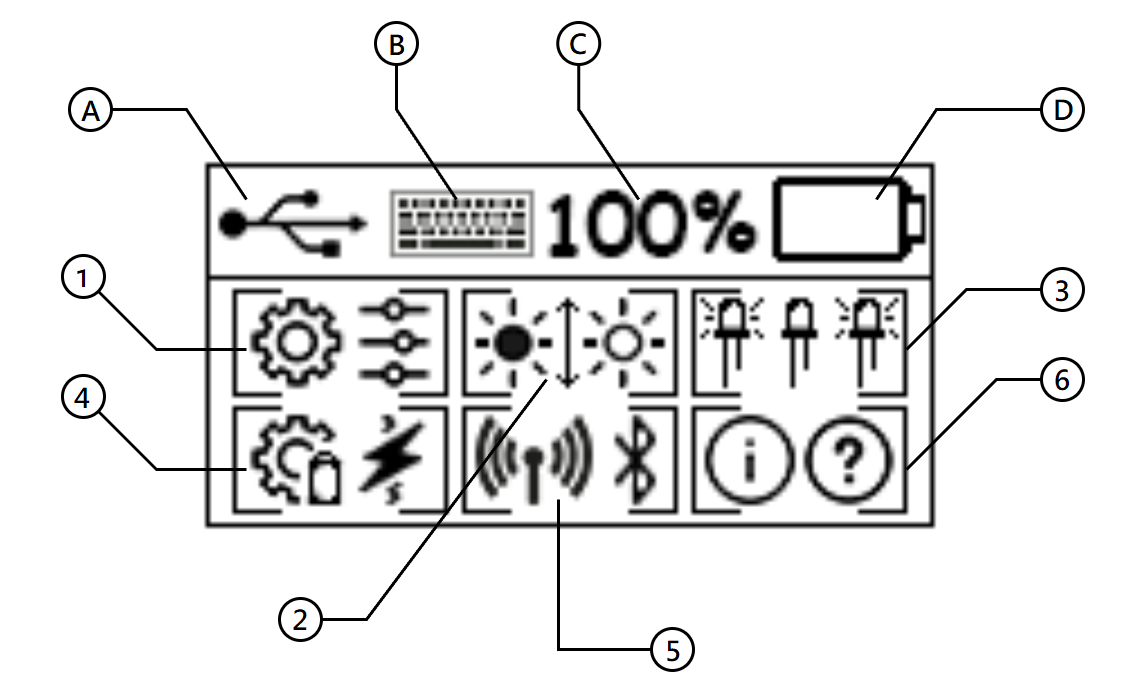
\includegraphics[width=1\textwidth]{imagenes/Capitulos/Cap07/PantallaMenuPrincipal.png}
\caption{Menú principal en la pantalla \gls{TFT} LCD 0.96''}
\label{fig:MenuPrincipal}
\end{figure}

\subsection{Menú}

El menú principal se compone de 6 opciones. Cada opción tiene un icono que corresponde a la categoría de la opción. Además, como se puede ver en la figura \ref{fig:MenuPrincipal} cada menú va a tener asociado un número. Este número es el número de la opción en el menú. Este número se va a usar para seleccionar la opción deseada. Para seleccionar una opción se va a usar la tecla Enter. Para moverse por el menú se van a usar las flechas de dirección. Para salir de una opción se va a usar la tecla Escape. Para volver al menú principal se va a usar la tecla ESC. Si se quiere entrar y salir del modo de configuración se va a usar la tecla Fn.

Los diferentes menús vienen señalados en la imagen por un número. Con este vamos a identificar al menú para poder explicar su funcionamiento. Los menús son los siguientes:
\begin{itemize}
\item 1. Ajustes
\item 2. Brillo
\item 3. Leds
\item 4. Batería y Energía
\item 5. Conexión
\item 6. Extra y Ayuda
\end{itemize}

\subsubsection{Ajustes}
Este menú se compone de varias opciones. En este menú se pueden ajustar los parámetros del funcionamiento del teclado. En este menú se pueden ajustar los parámetros de, activar y desactivar la pantalla, activar y desactivar el teclado, ajustar el tiempo de debounce del teclado y ajustar el idioma de la interfaz.

\subsubsection{Brillo}
Este menú se compone de los parámetros de brillo de la pantalla y de los \glsnocase{LED}s. En este submenú se pueden encontrar dos ajustes numéricos del 0 al 100. Estos ajustes son el brillo de la pantalla y el brillo de los \glsnocase{LED}s. También se pueden llegar a apagar los \glsnocase{LED}s y la pantalla mediante este submenú, ya que podemos poner el brillo a 0.

\subsubsection{\gls{LED}s}
Este menú se compone de los parámetros de los \glsnocase{LED}s. En este submenú se pueden encontrar los ajustes de activar o desactivar los \glsnocase{LED}s, el color de los \glsnocase{LED}s y el modo de los \glsnocase{LED}s y la velocidad de los \glsnocase{LED}s.

\subsubsection{Batería y Energía}
Este menú se compone de los parámetros de la batería y la energía. En este submenú se pueden encontrar los ajustes de la batería. Para este submenú encontramos activar o desactivar la batería y activar o desactivar el modo de ahorro de energía.

\subsubsection{Conexión}
Este menú se compone de los parámetros de la conexión. En este submenú se pueden encontrar los ajustes de la conexión. Podemos seleccionar activar el modo de \gls{Bluetooth} por preferencia, activar o desactivar el \gls{Bluetooth} y seleccionar como preferente el modo \gls{USB} sobre el modo \gls{Bluetooth}.

\subsubsection{Extra y Ayuda}
Este menú se compone de los parámetros de la ayuda y extras. En este submenú encontramos el restaurar la configuración de fábrica, el modo especial para las funciones programas por el usuario y dos opciones de información y ayuda.

\subsection{Barra de estado}

La barra de estado se compone de varios elementos. En la parte superior de la pantalla se puede ver el icono de la conexión (A), el icono del modo de funcionamiento del teclado (B), el porcentaje de batería restante (C) y el icono de la batería (D). Estos elementos se pueden ver en la figura \ref{fig:MenuPrincipal}.

\begin{itemize}
    \item \textbf{A}. Icono de la conexión: Este icono indica el estado de la conexión. Este puede alternar entre el icono de \gls{Bluetooth} y el icono de \gls{USB}.
    \item \textbf{B}. Icono del modo de funcionamiento del teclado: Este icono indica el estado del teclado. Este puede alternar entre el icono de teclado activado y el icono de configuración.
    \item \textbf{C}. Porcentaje de batería restante: Este porcentaje indica el porcentaje de batería restante que se actualiza cada 1 minuto.
    \item \textbf{D}. Icono de la batería: Este icono indica el estado de la batería. Este indica si la batería está cargando o si la batería está descargada. También indica la carga y posee colores para indicar el estado de la batería.
\end{itemize}

\section{Funcionalidad}

La funcionalidad de la placa se ha dividido en varios apartados. Cada apartado se ha dividido en varios estados. Cada estado se compone de varias funciones que se ejecutan en función del estado en el que se encuentre la placa. Para cambiar de un estado a otro se han usado variables de estado a lo largo del código. Estas variables nos indican en que modo estamos, en que menú estamos, en que opción estamos, si hemos cambiado alguna opción, si hemos pulsado algún botón, etc.

Lo que nos permite desde el bucle principal saber en qué estado nos encontramos de la ejecución del programa y que funciones debemos ejecutar en cada momento. A continuación se detallarán los diferentes estados de la placa y las funciones que se ejecutan en cada uno de los estados.

\subsection{Estados}
\subsubsection{Ahorro de energía}
El primer apartado es el ahorro de energía. En esta sección de código se comprueba si el flag de tiempo de ahorro de energía ha sido activado por interrupción hardware de un reloj. Si el flag está activado, se activa el modo de ahorro de energía y se desactiva la pantalla y los \glsnocase{LED}s. Si el flag está desactivado y el flag de que estamos durmiendo está activado, se despierta la pantalla y los \glsnocase{LED}s.

\subsubsection{Batería}
Aquí comprobamos si desde el gestor de interrupciones de la batería ha actualizado el valor de la misma. Si es valor ha variado, se actualiza el valor de la batería en la pantalla y se actualiza el icono de la batería.

\subsubsection{\gls{LED}s}
En esta sección se comprueba si los \glsnocase{LED}s están activados en la configuración y si el modo de los \glsnocase{LED}s es el modo de \glsnocase{LED}s programados por el usuario. Si es así se ejecuta el modo de \glsnocase{LED}s programados por el usuario. Si no se ejecuta el modo de \glsnocase{LED}s por defecto.

\subsubsection{Actualización de conexión}
En esta sección se comprueba si la conexión ha cambiado. Si ha cambiado, se actualiza el icono de la conexión y se actualiza el modo de conexión.

\subsubsection{Pantalla}
En esta sección se comprueba si la pantalla está activada. En el caso de estar activada, se comprueba que se ha cambiado el estado de la pantalla. En el caso afirmativo se actualiza la pantalla con la información necesaria. Además, de mostrar siempre la pantalla con el brillo seleccionado.

\subsubsection{Teclado}
Se comprueba primero que no estamos en el modo de teclas especiales o modo especial, ya que tendríamos que ejecutar la función especificada especial.
Si no estamos en el modo especial se procede a funcionar en modo normal del teclado, mientras se comprueba que el flag de la interrupción de la tecla Fn no este activado. Si está activado, se cambia el modo de teclado a configuración y se activa el flag de configuración.
En el modo configuración nos encontramos con los mismos, se comprueba que el flag de la interrupción de la tecla Fn no este activado. Si está activado se cambia el modo de teclado a normal y se desactiva el flag de configuración.

En el modo de configuración, cada vez que se pulsa una tecla se actualiza el valor de la tecla pulsada y se activa el flag de tecla pulsada, activando la función de actualizar la pantalla.

Estos estados se pueden ver en la figura \ref{fig:EstadosKeyboard} junto con la figura del diagrama de flujo del bucle principal \ref{fig:MainLoop}.

\begin{figure}[H]
    \centering
    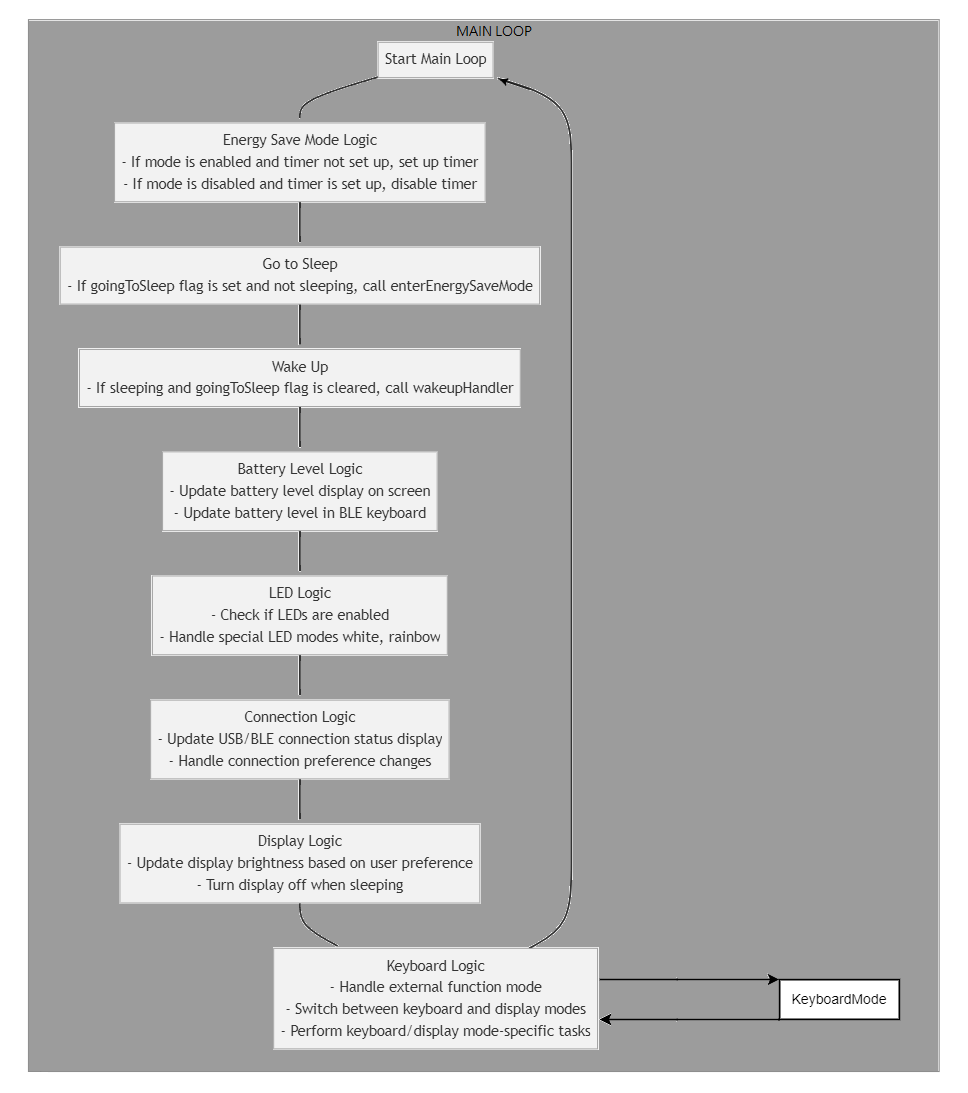
\includegraphics[width=1\textwidth]{imagenes/Capitulos/Cap07/MainLoop.png}
    \caption{Diagrama de Flujo del bucle principal}
    \label{fig:MainLoop}
\end{figure}

\begin{figure}[H]
    \centering
    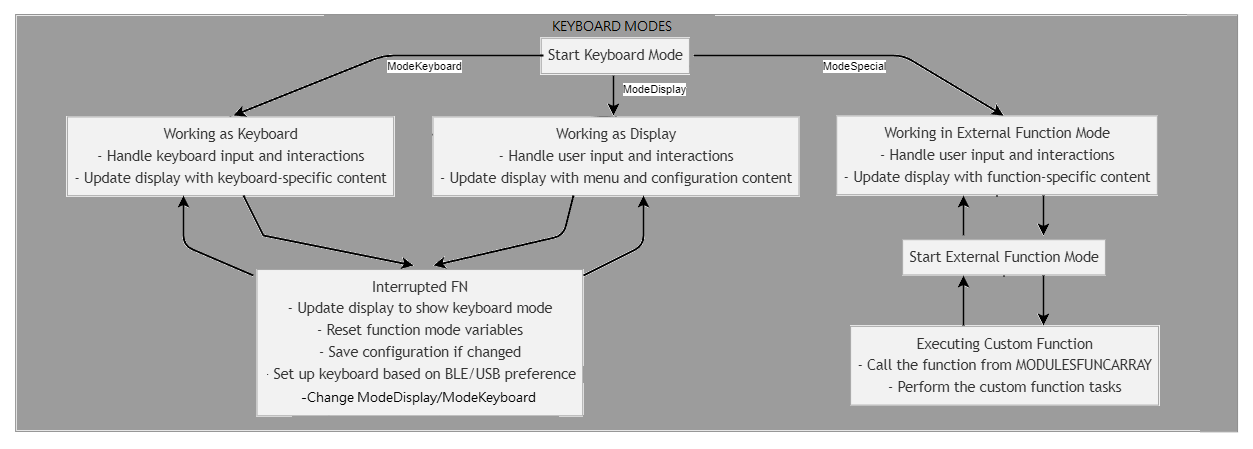
\includegraphics[width=1\textwidth]{imagenes/Capitulos/Cap07/EstadosKeyboard.png}
    \caption{Diagrama de Flujo de la secuencia de cambio de modo de teclado}
    \label{fig:EstadosKeyboard}
\end{figure}

\subsection{Conectividad}

Para la conectividad se ha decidido que sea independiente el modo \gls{Bluetooth} y el modo \gls{USB}. Para ello se ha creado un menú de configuración donde se puede seleccionar el modo de conexión preferente. Si se selecciona el modo \gls{USB} preferente, la placa se conectará por \gls{USB} siempre que esté conectado. Si se selecciona el modo \gls{Bluetooth} preferente, la placa se conectará por \gls{Bluetooth} siempre que esté conectado. Si no se selecciona ninguno de los dos modos, el teclado permanecerá desconectado. Se puede conectar por \gls{USB} y \gls{Bluetooth} a la vez, pero en tal caso tendrá preferencia el modo \gls{USB}.

\subsection{Leds}

Para los \glsnocase{LED}s se han creado varios modos de funcionamiento. Se ha creado el modo estático, donde el color seleccionado se mantiene fijo. El modo de color blanco y el modo arcoíris. Se podrán añadir más modos creando la función correspondiente y añadiéndola al menú de \glsnocase{LED}s. Revisar el apéndice \ref{ApendiceLeds} para más información.

\subsection{Macros}

Para los macros o funciones especiales, se tendrá que activar el modo desde el menú "Extra y ayuda". Ya que estas funciones serán creadas por el usuario y se tendran que añadir al código. Se podrán añadir más funciones creando la función correspondiente y añadiéndola al menú de macros. Revisar el apéndice \ref{ApendiceMacros} para más información.

\section{Boot}

Para poder cargar el código al microcontrolador se ha usado el conversor \gls{TTL} que se indicó en la sección \ref{DiseñoActualizaciones} se ha usado un conversor de nivel lógico para poder programar el chip mientras este se alimenta con el \gls{USB} 5.0 V y no con la batería.
El código una vez cargado en el microcontrolador se ejecutará en cuanto el chip revisa el voltaje necesario para funcionar. En este caso el chip se enciende en cuanto se conecta el \gls{USB} y se enciende la pantalla mostrando el logotipo del proyecto. Acto seguido se encienden los leds y se muestra el menú principal en el caso de estar activa la pantalla.

\begin{tcolorbox}[colback=red!11!white, colframe=red!50!white, title=Errores]
    Ver apartado de errores \ref{CorrienteInversa} y \ref{VoltajeRegulador} donde se explica por qué es necesario el conversor de nivel lógico.
\end{tcolorbox}
\chapter{Prototipos}

Durante el desarrollo del proyecto se han realizado varios prototipos para probar las diferentes funcionalidades del sistema. En este capítulo se describen los prototipos realizados y las pruebas realizadas. Se ha usado la placa de desarrollo ESP32S3-DevKitC-1 para realizar los prototipos en una protoboard junto con un \glsnocase{Multiplexor} DIP en vez de \gls{SMD} para facilitar la conexión de los cables. Durante el desarrollo de los prototipos se ha empleado solo un pequeño porcentaje de las teclas del producto final. Solo se han usado las teclas para controlar la pantalla y 3 teclas extra de funcionalidad, una letra, el shift y el espacio.


\section{Versiones}
Durante el desarrollo del proyecto se han realizado varias versiones de los prototipos. En este apartado se describen las diferentes versiones de los prototipos realizados.

\subsection{V1: Correcciones}
La primera de todas las versiones no contemplaba protocolo \glsnocase{Bluetooth} y tampoco poseía la pantalla \gls{OLED}. Se realizó para probar el funcionamiento de los interruptores y la \gls{PCB}. Se usó un microcontrolador Atmega32U4 y un \glsnocase{Multiplexor} DIP para facilitar la soldadura.

Principalmente, este prototipo fue para probar las dimensiones de la \gls{PCB} y la disposición de los interruptores. Además de la ergonomía del teclado. Esta primera versión se llama Tesseract \cite{Tesseract}.

\subsection{V2: Correcciones}
Esta versión fue una modificación del teclado Tesseract \cite{Tesseract} para cambiar la ergonomía, ya que era muy tosco y no era cómodo de usar. Se cambió la disposición del puerto \gls{USB}, ya que la primera versión usaba un \gls{USB} B y la nueva versión usa un \gls{USB} A.

\subsection{V3: Modificaciones}
Tras las ultimas dos versiones se decidió ampliar la funcionalidad creando el nuevo modelo ModernWood. Este incluiría una pantalla \gls{OLED} y un protocolo \gls{Bluetooth} para poder usar el teclado con dispositivos móviles. Se cambió el microcontrolador a un ESP32S3. Se cambió el material de la carcasa a madera y se añadió un difusor para los \gls{LED}s. Se añadió una batería de litio para poder usar el teclado sin cables y se cambió el conector \gls{USB} a un conector XS-12 para que fuera todavía más robusto.

\section{Problemas y Errores} \label{Errores}
En este apartado se describen los problemas y errores encontrados durante el desarrollo de los prototipos. Estos no han sido corregidos en las versiones de los prototipos, pero se han tenido en cuenta para el diseño del producto final.
\subsection{Corriente inversa en el regulador de tensión} \label{CorrienteInversa}
Es común que durante la operación normal del los componentes electrónicos, sobre todo los operados por personas, se produzcan errores en la conexión de los cables. Estos son errores que pueden ser fatales para los componentes electrónicos. Uno de estos errores es la conexión inversa de la alimentación. Para evitar que la corriente inversa dañe el regulador de tensión se ha añadido un diodo en la puerta del regulador de tensión.

Para evitar este problema, se coloca un diodo en la entrada del regulador de tensión. La función principal del diodo es bloquear cualquier corriente inversa que intente fluir hacia la entrada del regulador. El diodo permite el paso de corriente en una única dirección (de la entrada del regulador a la salida), y bloquea el flujo en la dirección opuesta. De esta manera, se protege el regulador de tensión de posibles daños por corriente inversa.

Además de su función de protección, el diodo también ayuda a estabilizar el funcionamiento del regulador de tensión en condiciones transitorias, como durante el encendido o apagado del circuito. Al evitar que la corriente inversa llegue al regulador, se minimizan las perturbaciones en la salida, asegurando una regulación de tensión más estable y fiable.

\subsection{Voltaje en la salida del regulador de tensión} \label{VoltajeRegulador}
Este problema, aunque parecido al anterior, la razón es totalmente diferente. En este caso, el problema ocurre cuando queremos alimentar el teclado mediante el programador \gls{TTL}. Ya que durante la programación del microcontrolador, el programador \gls{TTL} alimenta el teclado con 5 V o 3.3 V. Sin embargo, el regulador de tensión del teclado está diseñado para funcionar con una tensión de entrada de 3.3 V. Y además la alimentación del chip sería directa.

Por lo que el voltaje lo tendríamos en la puerta de salida del regulador de tensión. Por lo que para evitar lo que se conoce como voltaje ``\gls{BackfeedCurrent}'' en los reguladores se ha añadido de nuevo un diodo en la puerta de salida del regulador de tensión. Que permita el paso de la corriente de la puerta de salida del regulador a la puerta de entrada del regulador. Saltando el regulador de tensión.

Por esta razón, durante la programación de esta versión del teclado es necesario los conversores de nivel lógico para poder alimentar el teclado con 5 V y a su vez programarlo a 3.3 V y así evitar el problema del voltaje en la puerta de salida del regulador de tensión.

\newpage
\section{Montaje} \label{MontajeTeclado}
Esta sección describe el montaje del teclado en completo detalle. Se usará como explicación para el producto final y para saber el orden y la manera de proceder para el montaje del teclado. Ya que está diseñado para ser ensamblado en unos pasos concretos.

\begin{tcolorbox}[colback=red!11!white, colframe=red!50!white, title=Errores]
    Ver apartado de errores en el apéndice \ref{ApendiceEnsamblajeErrores} donde se detallan los errores encontrados durante el montaje y los cambios realizados a las diferentes partes del proyecto para corregirlos.
\end{tcolorbox}

\subsubsection{Soldadura de los componentes de la \gls{PCB}}
El primer paso es soldar los componentes de la \gls{PCB}. Se debe soldar los componentes de menor tamaño primero y los de mayor tamaño después. Se debe tener cuidado con la polaridad de los componentes y con la temperatura de la soldadura para no dañar los componentes, esta debe de ser 250 °C para la pasta de soldadura y 300 °C para el soldador manual. Se debe soldar los componentes en el siguiente orden:

\begin{enumerate}
    \item Resistencias
    \item Condensadores
    \item Diodos
    \item Chip Batería
    \item Microcontrolador
    \item Pantalla
    \item Interruptores
    \item Cables para \gls{USB}
\end{enumerate}

Para soldar los componentes \gls{SMD} se ha usado una pasta de soldadura de baja temperatura y una pistola de calor para fundir la pasta. Se ha usado un soldador manual para los componentes de mayor tamaño.

La pasta de soldadura se aplica junto con flux en las pistas de la \gls{PCB} y se coloca el componente encima. Se calienta la pasta con la pistola de calor hasta que se funda y se adhiera el componente a la \gls{PCB}. El propio estaño debe deslizarse hasta su posición en la pista y no debe ser empujado con la pistola de calor. Después de unos segundos de calentar, el chip debería haberse asentado en su posición. Se debe tener cuidado con la temperatura de la pistola de calor para no dañar los componentes.

Se ha de tener en cuenta la fuerza de la pistola de calor, ya que sí se pone la fuerza de la misma muy alta podría llegar a calentar otros componentes adyacentes y desoldarlos o dañarlos. \cite{SoldaduraSMD}

\subsubsection{Atornillado de los estabilizadores}
Una vez soldados los componentes de la \gls{PCB} se ha de colocar los estabilizadores en la \gls{PCB}. Para ello se ha de colocar los estabilizadores en los agujeros de la \gls{PCB} y atornillarlos con los tornillos correspondientes. Se ha de tener cuidado con la fuerza ejercida para no romper la \gls{PCB} ni los estabilizadores.

\subsubsection{Programación del microcontrolador}
El siguiente paso es programar el microcontrolador. Para ello se debe conectar el microcontrolador a un programador, en nuestro caso el FT232RL y cargar el \glsnocase{Firmware} en el microcontrolador. Se debe tener cuidado con la polaridad de los pines y con la conexión de los cables. Se debe conectar el programador al microcontrolador y al ordenador y cargar el \glsnocase{Firmware} en el microcontrolador. Se debe comprobar que el \glsnocase{Firmware} se ha cargado correctamente y que el microcontrolador funciona correctamente.

Para realizar esta tarea se emplearán los pines designados en la \gls{PCB} para la programación del microcontrolador.

\subsubsection{Difusor \glsnocase{LED}s}
Primero se ha de colocar el difusor sobre los \glsnocase{LED}s y se ha de atornillar con los tornillos pasantes sobre el difusor hasta una tuerca autoblocante que deberemos colocar en el otro extremo del tornillo. Se ha de tener cuidado con la fuerza ejercida para no romper el difusor ni la \gls{PCB}.

\subsubsection{Soldadura de cables para \gls{USB}}
Tanto en la placa base como en el conector XS-12 tenemos que soldar un cable de conexion Gx16-4 a la parte interna del conector y la parte hembra del conector a los pines correspondientes D+,D-,GND y VCC. Para ello se ha de soldar el cable a la parte interna del conector y a los pines de la placa base. Se ha de tener cuidado con la polaridad de los cables.

\subsubsection{Conector XS-12}
Con todos los pasos anteriores realizados tendriamos la \gls{PCB} lista para ser montada en la carcasa. Que de fabrica ya tiene las tuercas empotradas en sus agujeros correspondientes y el barnizado completo.

Una vez que tenemos la carcasa barnizada y con las tuercas empotradas deberemos colocar el conector XS-12 en su lugar correspondiente. Para ello se ha de colocar el conector en la carcasa y atornillarlo con los tornillos M1.7 x 5 mm de cabeza plana.

Después de atornillar el conector XS-12 y tener soldado los dos conectores Gx16 tendremos que conectarlos para dejarlos por debajo de la carcasa.

\subsubsection{Tornillos} \label{Tornillos}
Una vez colocado el difusor y el conector XS-12 se puede colocar la \gls{PCB} en la carcasa, para ello a lo largo de toda la carcasa se encuentran unos agujeros roscado en las tuercas empotradas M3 para atornillar la placa.

En la carcasa se deben colocar los espaciadores de 3 mm en los agujeros con las  y atornillarlos con un destornillador. Se debe tener cuidado con la fuerza ejercida para no mover o arrancar las tuercas empotradas pegadas con epoxi.

Una vez colocados se pondrá la \gls{PCB} sobre los espaciadores dejando la batería en la parte inferior. Se atornillará la \gls{PCB} a los espaciadores con los tornillos M3 de cabeza redondeada.

Una vez montada la \gls{PCB} sobre la carcasa se colocará el protector de metacrilato sobre los circuitos de la \gls{PCB}. Para poder atornillar el protector de metacrilato a la carcasa se han de colocar unos espaciadores de 5 mm en los agujeros correspondientes a los del protector. Estos agujeros no han debido ser atornillados previamente. Ya que los espaciadores de 5 mm servirán para poder fijar la \gls{PCB} a la carcasa y para poder servir de tuerca al protector de metacrilato.

Una vez colocados los espaciadores de 5 mm se colocará el protector de metacrilato sobre la \gls{PCB} y se atornillará con los tornillos M3 de cabeza redondeada a los espaciadores de 5 mm.

\subsubsection{\gls{Keycaps}}
Para colocar los \gls{Keycaps} en los interruptores se ha de colocar la tecla sobre el interruptor y presionar hasta que se mantenga sobre el interruptor. Se ha de tener cuidado con la fuerza ejercida para no romper el interruptor ni la \gls{PCB}.
\chapter{Validación}

En todos los proyectos de desarrollo de software y hardware es necesario realizar pruebas para comprobar que el sistema funciona correctamente. Aquí se destacarán las pruebas realizadas en el sistema para comprobar su correcto funcionamiento.

\section{Pruebas Eléctricas}
Para realizar todos los test y pruebas se ha hecho una plantilla tipica para rellenar, donde se le atribuye un nombre a la prueba, una descripción de la misma, como se realiza y el resultado obtenido. Esta se puede ver en la tabla \ref{Table:PruebasElectricas}.

\subsubsection{Prueba de Continuidad}

La prueba de continuidad se llevó a cabo utilizando un multímetro digital. Se verificó la continuidad en los circuitos de las teclas, los \gls{LED} indicadores y los cables de conexión. No se detectaron interrupciones en la continuidad, lo que indica una correcta conexión de los componentes.

\subsubsection{Prueba de Resistencia}

Se utilizaron instrumentos de medición adecuados para medir la resistencia eléctrica en diferentes puntos del teclado. Los valores de resistencia obtenidos se compararon con los rangos especificados en el diseño. Todos los componentes mostraron valores de resistencia dentro de los límites aceptables.

\subsubsection{Prueba de Corriente y Voltaje}

Se midió la corriente y el voltaje en varios puntos del circuito utilizando un amperímetro y un voltímetro. Los valores de corriente y voltaje se compararon con las especificaciones del diseño. Se observó un comportamiento adecuado de los circuitos, con corrientes y voltajes dentro de los rangos esperados.

\subsubsection{Prueba de Funcionamiento de los \gls{LED}}

Se realizó una prueba específica para verificar el funcionamiento de los \gls{LED} indicadores del teclado. Se encendieron y apagaron los \gls{LED} para confirmar que emitían luz de manera adecuada y que no presentaban fallos de conexión o funcionamiento.

\subsubsection{Prueba de Comunicación \gls{USB}}

Se verificó la comunicación entre el teclado y la computadora a través del puerto \gls{USB}. Se enviaron datos desde el teclado a la computadora para confirmar que la comunicación era estable y que no había pérdida de información.

\subsubsection{Prueba de Interferencias Electromagnéticas}

El teclado fue expuesto a fuentes de interferencias electromagnéticas para verificar su inmunidad a este tipo de interferencias. Se comprobó que el teclado seguía funcionando correctamente incluso en presencia de campos electromagnéticos externos no muy fuertes.

En resumen, las pruebas eléctricas confirmaron la integridad y el correcto funcionamiento del teclado diseñado, asegurando su fiabilidad y rendimiento en diferentes condiciones de operación.

\section{Pruebas en \gls{Windows}}

Las pruebas en el sistema operativo \gls{Windows} se llevaron a cabo para verificar la compatibilidad y funcionalidad del teclado diseñado en este entorno. A continuación, se detallan las pruebas realizadas. Se ha seguido una plantilla típica para rellenar, se puede ver en la tabla \ref{Table:PruebaSistemaWindows}.

\subsubsection{Prueba de Funcionamiento de las Teclas}

Se probó cada tecla del teclado para asegurar que todas fueran reconocidas correctamente por el sistema operativo \gls{Windows}. Se verificó que la pulsación de cada tecla generara la salida esperada en la pantalla y que no se produjeran errores de reconocimiento.

\subsubsection{Prueba de Comunicación \gls{USB}}

Se verificó la comunicación entre el teclado y la computadora a través del puerto \gls{USB} en el sistema operativo \gls{Windows}. Se confirmó que el teclado fuera detectado correctamente por el sistema y que la comunicación fuera estable y sin errores.

\subsubsection{Prueba de Funcionamiento de los \gls{LED}}

Se probó el funcionamiento de los \gls{LED} indicadores del teclado en el sistema operativo \gls{Windows}. Se verificó que los \gls{LED} se encendieran y apagaran correctamente según el estado de las funciones correspondientes.

\section{Pruebas en \gls{Linux}}

Las pruebas en el sistema operativo \gls{Linux} se realizaron para garantizar la compatibilidad y funcionalidad del teclado diseñado en este entorno. A continuación, se describen las pruebas realizadas. Se ha seguido una plantilla típica para rellenar, se puede ver en la tabla \ref{Table:PruebaSistemaLinux}.

\subsubsection{Prueba de Reconocimiento del Teclado}

Se verificó que el teclado fuera reconocido correctamente por el sistema operativo \gls{Linux} al conectarlo a la computadora. Se comprobó que el sistema asignara los \glsnocase{Controladores} adecuados y que el teclado estuviera listo para su uso sin necesidad de configuraciones adicionales.

\subsubsection{Prueba de Funcionamiento de las Teclas}

Se probó el funcionamiento de cada tecla del teclado en el sistema operativo \gls{Linux}. Se verificó que todas las teclas generaran la salida esperada en la pantalla y que no se produjeran errores de reconocimiento o asignación de caracteres.

\subsubsection{Prueba de Funcionamiento de los \gls{LED}}

Se verificó el funcionamiento de los \gls{LED} indicadores del teclado en el sistema operativo \gls{Linux}. Se confirmó que los \gls{LED} se encendieran y apagaran correctamente según el estado de las funciones correspondientes.

En resumen, las pruebas realizadas en ambos sistemas operativos confirmaron la compatibilidad y funcionalidad del teclado diseñado en diferentes entornos de software.

\begin{table}[h]
\small
\begin{tabular}{|l|p{2cm}|p{2.5cm}|p{3cm}|}
\hline
Nombre & Descripción & Como se realiza & Resultado \\
\hline
Continuidad & Verifica la continuidad & Utilizando un multímetro digital & Sin interrupciones \\
\hline
Resistencia & Mide la resistencia eléctrica & Con instrumentos de medición adecuados & Valores dentro de los límites aceptables \\
\hline
Corriente y Voltaje & Mide la corriente y el voltaje & Utilizando un amperímetro y un voltímetro & Corriente y voltaje dentro de los rangos esperados \\
\hline
\gls{LED}S & Verifica el funcionamiento de los \gls{LED} & Encendiendo y apagando los \gls{LED} & Emisión de luz adecuada \\
\hline
\gls{USB} & Verifica la comunicación \gls{USB} & Enviando datos desde el teclado a la computadora & Comunicación estable sin pérdida de información \\
\hline
\gls{EMI} & Prueba la inmunidad a interferencias electromagnéticas & Exponiendo el teclado a fuentes de \gls{EMI} & Funcionamiento correcto incluso en presencia de campos electromagnéticos externos \\
\hline
\end{tabular}
\caption{Pruebas eléctricas realizadas}
\label{Table:PruebasElectricas}
\end{table}

\begin{table}[!htb]
\small
\begin{tabular}{|l|p{3cm}|p{3.5cm}|l|}
\hline
Nombre           & Descripción                                               & Como se realiza                                    & Resultado \\ \hline
Reconocimiento   & Verifica el reconocimiento de las teclas en \gls{Windows}        & Se prueba cada tecla del teclado en \gls{Windows}        & OK         \\ \hline
Envío de Teclas  & Verifica el envío de teclas desde el teclado en \gls{Windows}    & Se verifica la comunicación \gls{USB} en \gls{Windows}         & OK         \\ \hline
\gls{LED}S             & Verifica el funcionamiento de los \gls{LED} en \gls{Windows}           & Se prueba el encendido y apagado de los \gls{LED}        & OK         \\ \hline
\end{tabular}
\caption{Pruebas en \gls{Windows}}
\label{Table:PruebaSistemaWindows}
\end{table}

\phantom{Espacio}
\begin{table}[!htb]
\small
\begin{tabular}{|l|p{3cm}|p{3.5cm}|l|}
\hline
Nombre           & Descripción                                               & Como se realiza                                    & Resultado \\ \hline
Reconocimiento   & Verifica el reconocimiento de las teclas en \gls{Linux}        & Se prueba cada tecla del teclado en \gls{Linux}        & OK         \\ \hline
Envío de Teclas  & Verifica el envío de teclas desde el teclado en \gls{Linux}    & Se verifica la comunicación \gls{USB} en \gls{Linux}         & OK         \\ \hline
\gls{LED}S             & Verifica el funcionamiento de los \gls{LED} en \gls{Linux}           & Se prueba el encendido y apagado de los \gls{LED}        & OK         \\ \hline
\end{tabular}
\caption{Pruebas en \gls{Linux}}
\label{Table:PruebaSistemaLinux}
\end{table}
    
\chapter{Mejoras}

\section{Posibles mejoras}
\subsection{Software}
\subsection{Hardware}
\subsection{Materiales}
\section{Consideraciones Personales}
\chapter{Conclusiones}

Aunque este proyecto empezase hace unos meses. Las primeras versiones de este empezaron hace años. Desde que empecé a interesarme por la programación y la electrónica, siempre he querido hacer un teclado por las razones que expuse en mi motivación. Por eso, aunque no haya sido un proyecto fácil, ha sido un proyecto muy gratificante y que me ha enseñado mucho. Y más aún cuando con cada versión me doy cuenta de que puedo hacer un teclado mejor. Y que dentro de un tiempo, pueda mirar este proyecto, tomar lo que he aprendido y las posibles mejoras que propuse y volver a empezar de nuevo el viaje.

Durante el proceso de diseño y desarrollo, se han enfrentado varios desafíos y se han tomado decisiones importantes para garantizar la calidad y el rendimiento del teclado. Se han realizado pruebas exhaustivas para verificar la funcionalidad y la compatibilidad del teclado en diferentes entornos, lo que ha permitido identificar áreas de mejora y optimización. Uno de los aspectos más destacados de este proyecto ha sido la oportunidad de aplicar conocimientos teóricos aprendidos en un entorno práctico.

En cuanto a los resultados obtenidos, el teclado diseñado ha demostrado ser funcional, robusto y altamente adaptable a las necesidades del usuario. Aunque todavía hay mucho margen para mejorar, el teclado ha demostrado ser una alternativa viable a los teclados convencionales y ofrece una serie de ventajas y características únicas que lo hacen atractivo para una amplia gama de usuarios.

En conclusión, este proyecto ha sido una experiencia enriquecedora que ha permitido aplicar conocimientos teóricos en un contexto práctico y desarrollar habilidades técnicas y profesionales. El teclado diseñado representa un avance significativo en mi camino hacía alcanzar la excelencia en estos campos y me ha motivado a seguir explorando nuevas oportunidades y desafíos en el futuro. El proyecto de los teclados mecánicos personalizados ha sido un largo camino durante estos años, pero cada vez que avanzo no puedo esperar a volver a tener ganas de volver a empezar de nuevo para mejorar lo que ya he hecho.

\section{Trabajo futuro}
Con este proyecto terminado ya estoy pensando en futuras versiones del teclado. Aunque este teclado ya tiene muchas funcionalidades que me gustaría tener en un teclado, hay algunas funcionalidades que me gustaría añadir en futuras versiones del teclado. Algunas de las mejoras que me gustaría añadir en futuras versiones del teclado para que este verdaderamente sea una obra de ingeniería y diseño son; los \gls{Switches} ópticos y magnéticos, la implementación de un sistema de carga inalámbrica, la adición de un sistema de actualización de firmware over-the-air (OTA), desarrollar un driver que permita personalizar el teclado de forma gráfica desde un programa en el ordenador y la implementación de módulos complejos como diccionarios de palabras, calculadoras o control de dispositivos IoT.
%\chapter{Viabilidad Comercial}

El presente capítulo tiene como objetivo analizar la viabilidad comercial de un teclado customizado de alta gama, diseñado específicamente para satisfacer las necesidades del mercado español. Este teclado se distingue por varias características innovadoras, incluyendo un diseño sin plate, la incorporación de una pantalla OLED, una conectividad Bluetooth y la disposición 105 ISO español, lo que lo convierte en una opción única en el mercado.

La viabilidad comercial de un producto no solo depende de su diseño y funcionalidad, sino también de una serie de factores que abarcan desde el análisis del mercado hasta los costos asociados con su producción y comercialización. En este capítulo, se llevará a cabo un análisis exhaustivo que abarca diversos aspectos cruciales para determinar la potencial aceptación y éxito del teclado en el mercado.

Primero, se realizará un análisis del proyecto, donde se evaluarán los objetivos, la propuesta de valor y los principales beneficios del teclado. A continuación, se desarrollarán estudios de mercado que identificarán las características del mercado objetivo, incluyendo el tipo de mercado, el ámbito geográfico, la evolución del mercado, la fase en la que se encuentra, así como los clientes y proveedores potenciales. Además, se presentarán previsiones futuras basadas en tendencias actuales y proyecciones de crecimiento.

El análisis FODA (Fortalezas, Oportunidades, Debilidades y Amenazas) proporcionará una visión integral de los factores internos y externos que pueden influir en el éxito del teclado. Este análisis permitirá identificar las ventajas competitivas del producto, así como los desafíos que podrían surgir y las oportunidades que se podrían aprovechar.

Asimismo, se examinarán los costos asociados al proyecto, incluyendo los costos de producción, comercialización, administración, financiamiento e impuestos. Este análisis financiero es esencial para entender la inversión requerida y los márgenes de beneficio esperados.

Los aspectos legales también serán considerados, incluyendo los registros necesarios para operar la empresa y proteger la propiedad intelectual del producto. Finalmente, se diseñará una estrategia de marketing que abarcará la publicidad, promoción, distribución, ventas y posibles alianzas estratégicas para asegurar una presencia efectiva en el mercado.

En resumen, este capítulo proporcionará una visión detallada y estructurada de todos los elementos que intervienen en la viabilidad comercial del teclado fabricado customizado de alta gama, con el fin de evaluar su potencial de éxito en el mercado español.

\section{Análisis del proyecto}

El proyecto del teclado customizado de alta gama se centra en la creación de un dispositivo de entrada de alta calidad, diseñado para satisfacer las necesidades específicas de los usuarios en el mercado español. Este teclado se caracteriza por varias innovaciones y especificaciones técnicas que lo diferencian de los productos disponibles actualmente en el mercado.

\subsection{Objetivos del proyecto}

El objetivo principal del proyecto es desarrollar un teclado que combine ergonomía, funcionalidad y personalización, ofreciendo una experiencia de usuario superior. Los objetivos específicos incluyen:

\begin{itemize}
    \item Fabricar un teclado sin plate, lo que permite una mayor flexibilidad y un mantenimiento más sencillo.
    \item Incorporar una pantalla OLED, permitiendo una interacción más dinámica y visualmente atractiva.
    \item Diseñar el teclado con la disposición 105 ISO español, garantizando su adaptabilidad y comodidad para los usuarios de habla hispana.
    \item Utilizar materiales de alta calidad para asegurar la durabilidad y el rendimiento del teclado.
    \item Ofrecer opciones de personalización para los usuarios, como la elección de interruptores, keycaps y carcasa y así como la posibilidad de programar macros y efectos de iluminación.
\end{itemize}

\subsection{Propuesta de valor}

La propuesta de valor del teclado se basa en ofrecer un producto premium que destaca por su calidad, diseño y funcionalidad. Las principales ventajas que se ofrecen a los usuarios incluyen:

\begin{itemize}
    \item \textbf{Interactividad avanzada:} La pantalla LED permite personalizar y visualizar información en tiempo real, mejorando la interacción con el teclado.
    \item \textbf{Durabilidad:} El uso de materiales de alta calidad asegura que el teclado tenga una larga vida útil, resistiendo el uso intensivo.
    \item \textbf{Exclusividad:} Al ser un producto fabricado bajo demanda, cada teclado es único, ofreciendo a los usuarios una sensación de exclusividad.
    \item \textbf{Experiencia de usuario superior:} Las características personalizables y la interactividad avanzada mejoran la satisfacción del usuario.
    \item \textbf{Valor estético:} El diseño elegante y la posibilidad de personalización hacen que el teclado también sea un objeto estético.
    \item \textbf{Compatibilidad:} El teclado está diseñado para ser compatible con una amplia gama de sistemas operativos y dispositivos, asegurando su versatilidad de uso.
    \item \textbf{Robustez:} La construcción sólida y los materiales de alta calidad garantizan que el teclado pueda soportar un uso intensivo y prolongado.
    \item \textbf{Personalización:} Los usuarios pueden personalizar el teclado según sus preferencias, creando una experiencia de tecleo única.
    \item \textbf{Reparabilidad:} El diseño sin plate facilita la reparación y el mantenimiento del teclado, prolongando su vida útil.
    \item \textbf{Conectividad:} La conectividad Bluetooth permite una mayor flexibilidad y movilidad para los usuarios.
\end{itemize}

\subsection{Evaluación de la demanda}

Para asegurar el éxito comercial del teclado, es crucial evaluar la demanda potencial en el mercado. La demanda puede ser influenciada por varios factores:

\begin{itemize}
    \item \textbf{Tendencias del mercado:} El aumento en la popularidad de los productos de tecnología personalizables y de alta calidad sugiere una demanda creciente para teclados premium.
    \item \textbf{Segmentación del mercado:} Identificar los segmentos de mercado, como gamers, profesionales de oficina y entusiastas de la tecnología, que estarían interesados en un teclado de estas características.
    \item \textbf{Competencia:} Analizar la competencia existente y cómo el teclado customizado de alta gama se posiciona frente a otros productos similares.
    \item \textbf{Precio:} Evaluar la disposición a pagar de los consumidores por un producto premium y personalizable.
\end{itemize}

\subsection{Plan de desarrollo}

El plan de desarrollo del proyecto contempla varias etapas clave para asegurar la viabilidad comercial del teclado:

\begin{enumerate}
    \item \textbf{Investigación y desarrollo:} Esta etapa incluye el diseño del teclado, la selección de materiales y componentes, y la creación de prototipos.
    \item \textbf{Pruebas y validación:} Se realizarán pruebas exhaustivas para asegurar la calidad, durabilidad y funcionalidad del teclado.
    \item \textbf{Producción:} Una vez validados los prototipos, se procederá a la producción en pequeñas series, garantizando el control de calidad.
    \item \textbf{Marketing y lanzamiento:} Se desarrollará una estrategia de marketing para promocionar el teclado y se planificará su lanzamiento al mercado.
    \item \textbf{Distribución:} Se establecerán canales de distribución para asegurar que el producto llegue eficientemente a los consumidores.
\end{enumerate}

\section{Estudios de mercado}

\subsection{Características del mercado}

Para evaluar la viabilidad comercial, es crucial analizar las características del mercado en el que se planea introducir. Este análisis permitirá entender el contexto en el que el producto competirá y las oportunidades disponibles. Para ello se va a buscar información sobre el tipo de mercado, el ámbito geográfico, la evolución del mercado, la fase en la que se encuentra, los clientes potenciales y los proveedores. Se van a utilizar fuentes de información como estudios de mercado, informes sectoriales y datos de la competencia. \cite{Comercial1} \cite{Comercial2} \cite{Comercial3}

\subsubsection{Tipo de mercado a intervenir}

El mercado objetivo para este proyecto es el de productos de lujo, \textit{DIY} (Do It Yourself) y bajo demanda. Este segmento de mercado se caracteriza por consumidores que buscan productos de alta calidad, exclusivos y personalizables. Los usuarios de este mercado valoran la experiencia y la exclusividad del producto, así como la posibilidad de personalización según sus preferencias. Este a su vez es un mercado de nicho, con una demanda específica y un alto potencial de crecimiento con una competencia limitada.

\subsubsection{Ámbito geográfico}

El ámbito geográfico principal para la comercialización del teclado será España y Latinoamérica. Sin embargo, dada la naturaleza del producto y el creciente interés global por los productos \textit{DIY} y de lujo, también se considerará la expansión a otros mercados como el Japonés y Ruso, ya que estos comparten la disposición de teclado ISO y la demanda de productos de alta calidad y personalizables.

\subsubsection{Evolución del mercado}

El mercado de teclados personalizados y de alta gama ha experimentado un crecimiento significativo en los últimos años. Con el aumento del teletrabajo y la demanda de equipos de calidad para mejorar la productividad y la experiencia del usuario, los consumidores están cada vez más dispuestos a invertir en productos de tecnología avanzada y personalizados. Esto se puede ver reflejado en el crecimiento de las ventas de teclados mecánicos, ya que estos ofrecen una mejor experiencia y hay una tendencia creciente hacia esas sensaciones y características de los teclados mecánicos \ref{fig:RevenueWW}.

\begin{figure}[H]
\centering
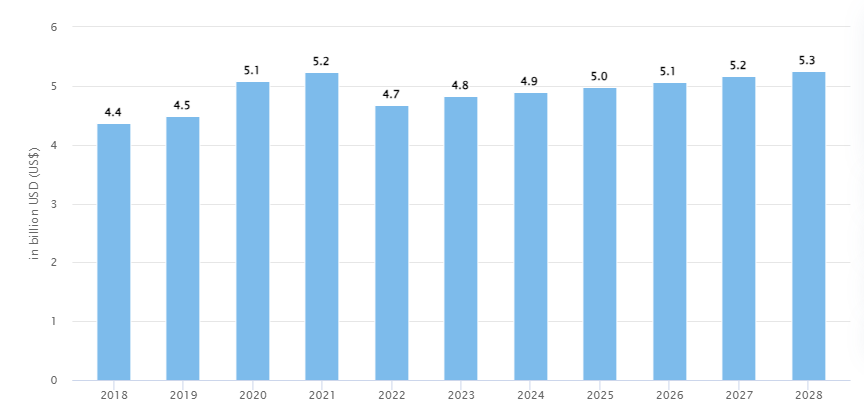
\includegraphics[width=1\textwidth]{imagenes/Capitulos/Cap12/RevenueKeyboardsWW.png}
\caption{Ganancia global del mercado de teclados mecánicos \cite{Comercial1}.}
\label{fig:RevenueWW}
\end{figure}

Actualmente, el mercado de teclados personalizados y de lujo se encuentra en una fase de crecimiento. La innovación constante y la introducción de nuevas tecnologías, como los teclados sin plate y las pantallas LED integradas, están impulsando la demanda y atrayendo a un número creciente de entusiastas de la tecnología y profesionales \ref{fig:VolumenWW}.

\begin{figure}[H]
\centering
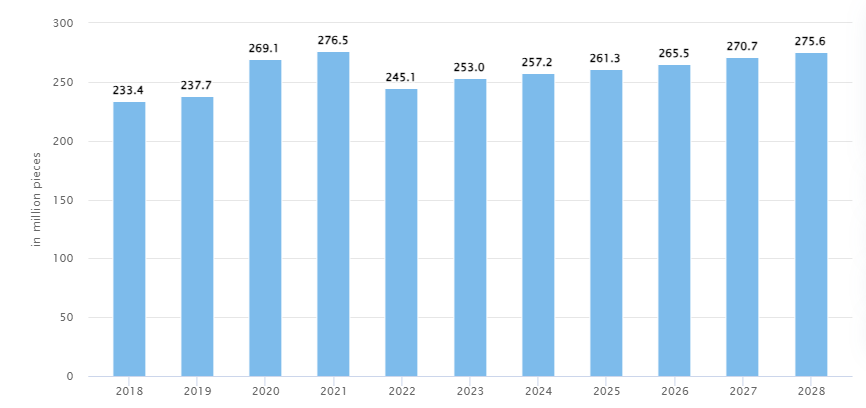
\includegraphics[width=1\textwidth]{imagenes/Capitulos/Cap12/VolumenKeyboard.png}
\caption{Volumen global del mercado de teclados mecanicos \cite{Comercial1}.}
\label{fig:VolumenWW}
\end{figure}

\subsubsection{Clientes}

Los clientes potenciales para este teclado incluyen:

\begin{itemize}
\item \textbf{Gamers:} Buscan teclados con alta respuesta y personalización.
\item \textbf{Profesionales de oficina:} Valoran la ergonomía y la durabilidad del teclado.
\item \textbf{Entusiastas de la tecnología:} Interesados en productos innovadores y personalizables.
\item \textbf{Consumidores de productos de lujo:} Buscan exclusividad y alta calidad.
\end{itemize}

\subsubsection{Proveedores}

Para la fabricación del teclado, se trabajará con proveedores de componentes electrónicos, materiales de alta calidad y servicios de fresado. Se han encontrado proveedores a muy bajo coste tanto para minoristas y mayoristas. Para los componentes electrónicos tendríamos la empresa LCSC y junto con su filial JLCPCB para la fabricación de PCBs.
Para los materiales de alta calidad se ha encontrado la empresa Keyreative que ofrece keycaps de alta calidad y personalizables.
Para los servicios de fresado se ha encontrado empresas locales que ofrecen servicios de fresado a bajo coste.
Para toda la logística y distribución se ha encontrado la empresa DHL O GLS que ofrece servicios de envío a nivel mundial a precios competitivos.

\subsubsection{Estrategia}

Dando que sería necesario un gran capital para poder fabricar los teclados en masa, se ha decidido que la mejor estrategia sería la de fabricar los teclados bajo demanda. De esta manera se podría ofrecer un producto de alta calidad y personalizable a un precio competitivo. Además de no tener que tener un gran almacén con gran stock. Esto también abaratará los costes de producción y almacenamiento. La estrategia más viable para este caso sería usar páginas de founding como Kickstarter o Indiegogo para poder financiar la producción de los teclados, así como para poder medir la demanda del producto y poder ajustar la producción a la demanda.

\subsubsection{Previsiones futuras}

Se espera que la demanda de teclados personalizados y de alta gama continúe creciendo en los próximos años. Las tendencias indican una preferencia creciente por productos que combinan funcionalidad, personalización y diseño exclusivo. Además, la expansión del mercado \textit{DIY} y el aumento del teletrabajo seguirán impulsando esta demanda.

\subsection{Análisis FODA}

\subsubsection{Fortalezas}

\begin{itemize}
    \item \textbf{Calidad y durabilidad:} Uso de materiales premium y diseño robusto.
    \item \textbf{Personalización:} Opciones de interruptores y keycaps intercambiables.
    \item \textbf{Innovación:} Diseño sin plate y pantalla LED integrada.
    \item \textbf{Exclusividad:} Producto customizado de alta gama, único para cada usuario.
\end{itemize}

\subsubsection{Oportunidades}

\begin{itemize}
    \item \textbf{Crecimiento del mercado:} Aumento de la demanda de productos de lujo y personalizados.
    \item \textbf{Expansión geográfica:} Potencial para llegar a mercados internacionales.
    \item \textbf{Nuevas tecnologías:} Incorporación de innovaciones tecnológicas adicionales.
\end{itemize}

\subsubsection{Debilidades}

\begin{itemize}
    \item \textbf{Costo elevado:} El precio total de 249,54 \euro~puede ser una barrera para algunos consumidores.
    \item \textbf{Tiempo de fabricación:} Producción artesanal puede ser más lenta comparada con métodos industriales.
\end{itemize}

\subsubsection{Amenazas}

\begin{itemize}
    \item \textbf{Competencia:} Otros fabricantes de teclados personalizados y de alta gama.
    \item \textbf{Cambios en las tendencias de consumo:} Preferencias de los consumidores pueden cambiar.
\end{itemize}

\section{Costos, legal, marketing}

Un apartado importante para la viabilidad comercial de un producto es el análisis de los costos asociados con su producción, comercialización y distribución. Además, es necesario considerar los aspectos legales y de marketing para asegurar el cumplimiento de las regulaciones y la promoción efectiva del producto en el mercado.

\subsection{Costos}

Todos los costes por unidad vienen detallados en la tabla \ref{Table:ComponentesMontaje}, \ref{Table:ComponetesElectronicos}, \ref{Table:ServiciosHerramientas}. A estos costes habría que sumarle los costes de logística y distribución. Además de los de marketing y publicidad. Aunque estos al ser costes variables no se pueden calcular con exactitud. Y dependerían bastante de la demanda del producto que se haría a partir de la campaña de founding. Por lo que se ha decidido no incluirlos en el cálculo de los costes.

\subsubsection{Costos de producción} \label{SeccionCostosProduccion}

Dado que estos costos han sido calculados por unidad sin tener en cuenta la cantidad y sin tener en cuenta las ganancias. Fácilmente podemos usar este precio de referencia para los siguientes cálculos. El coste por unidad es de 249,54 \euro. Este precio incluye todos los componentes y servicios necesarios para la fabricación del teclado. (Estos podrían llegar a ser menor al aumentar la cantidad de unidades fabricadas).

\subsubsection{Costos de comercialización}

Los costos de comercialización incluyen todos los gastos necesarios para llevar el producto al mercado y hacerlo llegar a los consumidores. Estos costos pueden incluir:

\begin{itemize}
    \item \textbf{Publicidad:} Gastos en campañas publicitarias, tanto online como offline.
    \item \textbf{Promoción:} Descuentos, ofertas especiales y actividades promocionales.
    \item \textbf{Distribución:} Costos asociados al envío y manejo del producto.
    \item \textbf{Plataformas de venta:} Comisiones y tarifas de plataformas de venta online.
    \item \textbf{Marketing digital:} Costos de SEO, SEM, redes sociales y marketing de contenidos.
\end{itemize}

Para estimar los costos de comercialización, se considera un porcentaje del precio de venta. En este caso, se estima que los costos de comercialización representan aproximadamente el 20\% del precio de venta. Este porcentaje sigue un razonamiento basado en la naturaleza del producto, los canales de comercialización y competencia en el mercado. Y por supuesto basado en ejemplos de productos similares en el mercado.

\subsubsection{Cálculo del costo de comercialización}
Se ha investigado y se han encontrado ejemplos de productos similares en plataformas de venta como Amazon, Etsy, y tiendas especializadas. Estas plataformas suelen implicar comisiones que varían entre el 10\% y el 15\% del precio de venta. Comparando con productos similares en la industria tecnológica, especialmente aquellos de nicho y personalizados, es común asignar entre un 15\% y un 25\% del precio de venta a los costos de comercialización. Este rango permite cubrir adecuadamente todos los aspectos necesarios para lanzar y mantener un producto en el mercado.

Por lo tanto, se ha estimado que un 20\% del precio de venta es un valor razonable para los costos de comercialización. Este porcentaje no comprometerá la viabilidad del proyecto, ya que la estrategia a seguir es de financiación bajo demanda.

\begin{equation}
\text{Costo de comercialización} = 0,20 \times 249,54 \euro = 49.91 \euro
\end{equation}

\subsubsection{Costos de administración}
Ya que este proyecto lo estaría llevando a cabo yo solo, y los costes asociados al personal ya están incluidos en los costes de producción. No habría costes adicionales asociados a la administración.

\subsubsection{Costos de financiamiento}
Como la estrategia elegida es la de financiación bajo demanda, no habría costes asociados a financiamiento. Ya que el capital necesario para la producción del teclado se obtendría a través de la campaña de founding y vendría de los propios clientes, estos pagarían por adelantado el producto.

Aunque Kickstarter e Indiegogo cobran una comisión por el uso de sus plataformas, esta comisión se deduce directamente del dinero recaudado y es del 5\% en Kickstarter \cite{ComisionKickStarer} y de máximo 8\% en Indiegogo \cite{ComisionIndiegogo}. Por lo que no se considera un coste adicional.
\subsubsection{Costos de impuestos}

Los costos de impuestos incluyen todos los tributos que la empresa debe pagar, tales como:

\begin{itemize}
\item \textbf{impuesto sobre la renta:} Impuesto sobre las ganancias de la empresa.
\item \textbf{Impuesto al valor agregado (IVA):} Impuesto sobre las ventas de productos.
\item \textbf{Contribuciones sociales:} Impuestos relacionados con los empleados. (No aplicable en este caso)
\end{itemize}

Dado que el iva en España es del 21\% \cite{IVA}, el coste de impuestos sería de y el impuesto sobre la renta es del 24\% \cite{ImpuestoRenta}, el coste de impuestos sería de:

\begin{equation}
\text{Costo de impuestos} = 0,21 \times 249,54 \euro + 0,24 \times 249,54 \euro = 112.29 \euro
\end{equation}

\subsection{Total de costos}
Computando todos los costes, el coste total por unidad seria de:

\begin{equation}
\text{Costo total} = 249,54 \euro + 49,91 \euro + 112,29 \euro = 411,74 \euro
\end{equation}

Este sería el precio máximo que se podría vender el teclado sin tener en cuenta las ganancias. Aunque este precio podría ser menor al aumentar la cantidad de unidades fabricadas, llegaría a poder disminuirse hasta un 35\% para más de 1000 unidades fabricadas y de 30\% para más de 500 unidades fabricadas.
El precio total de coste de una unidad sería de 411,74 \euro.
El precio total de coste de 100 unidades sería de 337.63 \euro.
El precio total de coste de 500 unidades sería de 288.22 \euro.
El precio total de coste de 1000 unidades sería de 267.63 \euro.

\subsection{Aspectos legales}

La consideración de los aspectos legales es fundamental para asegurar que el negocio del teclado customizado de alta gama opere dentro del marco legal adecuado y proteja sus activos intelectuales. A continuación, se describen los pasos necesarios para cumplir con las regulaciones legales y proteger la propiedad intelectual del producto.

\subsubsection{Registro de la empresa}

Para asegurar que el capital personal no corra peligro, se recomienda establecer la empresa como una \textbf{Sociedad de Responsabilidad Limitada (S.L.)}, donde los socios no responden personalmente por las deudas sociales, sino únicamente con el capital aportado.

\textbf{Proceso jurídico para darse de alta en el Registro Mercantil:}

\begin{enumerate}
    \item \textbf{Certificación negativa del nombre:} Solicitar una certificación negativa del nombre de la sociedad en el Registro Mercantil Central para asegurarse de que el nombre elegido no esté ya registrado.
    \item \textbf{Redacción de los estatutos sociales:} Elaborar los estatutos sociales que regirán la empresa. Estos deben incluir la denominación social, el objeto social, el domicilio social, el capital social y la estructura de administración de la sociedad.
    \item \textbf{Apertura de una cuenta bancaria:} Depositar el capital social mínimo (3.000 euros) en una cuenta bancaria a nombre de la futura sociedad. El banco emitirá un certificado del depósito.
    \item \textbf{Otorgamiento de la escritura pública:} Acudir a una notaría para otorgar la escritura pública de constitución de la sociedad, que debe incluir la certificación negativa del nombre, los estatutos sociales y el certificado del banco.
    \item \textbf{Obtención del Número de Identificación Fiscal (NIF) provisional:} Solicitar el NIF provisional en la Agencia Tributaria, presentando la escritura de constitución y el modelo 036 de alta censal.
    \item \textbf{Inscripción en el Registro Mercantil:} Presentar la escritura pública de constitución en el Registro Mercantil de la provincia donde la empresa tendrá su domicilio social. Una vez inscrita, la sociedad adquirirá plena personalidad jurídica.
    \item \textbf{Obtención del NIF definitivo:} Con la inscripción en el Registro Mercantil, se debe acudir nuevamente a la Agencia Tributaria para obtener el NIF definitivo.
    \item \textbf{Alta en el Impuesto de Actividades Económicas (IAE):} Registrar la empresa en el IAE, obligatorio para realizar actividades comerciales en España.
\end{enumerate}

\subsubsection{Registro de la marca}

El registro de la marca es crucial para proteger el nombre y el logotipo del teclado. Los pasos incluyen:

\begin{enumerate}
    \item \textbf{Búsqueda de antecedentes:} Realizar una búsqueda para asegurarse de que la marca no esté ya registrada por otra empresa.
    \item \textbf{Solicitud de registro:} Presentar una solicitud de registro ante la Oficina Española de Patentes y Marcas (OEPM).
    \item \textbf{Revisión y publicación:} La OEPM revisará la solicitud y, si no hay objeciones, publicará la marca en el Boletín Oficial de la Propiedad Industrial (BOPI).
    \item \textbf{Registro internacional:} Considerar el registro internacional de la marca si se planea expandir el mercado fuera de España, utilizando el Sistema de Madrid de la Organización Mundial de la Propiedad Intelectual (OMPI).
\end{enumerate}

\subsubsection{Registro de la patente}

Si el teclado incorpora innovaciones técnicas únicas, puede ser necesario patentar esas innovaciones:

\begin{enumerate}
    \item \textbf{Preparación de la solicitud:} Documentar detalladamente la innovación técnica, incluyendo dibujos y descripciones técnicas.
    \item \textbf{Presentación de la solicitud:} Presentar la solicitud de patente ante la OEPM.
    \item \textbf{Examen de fondo:} La OEPM realizará un examen de fondo para evaluar la novedad y la aplicabilidad industrial de la invención.
    \item \textbf{Concesión de la patente:} Si la solicitud es aprobada, se concede la patente, que proporciona protección legal durante un periodo de 20 años.
\end{enumerate}

\subsubsection{Registro de derechos de autor}

Para proteger el software y otros elementos creativos del teclado, se debe considerar el registro de derechos de autor:

\begin{enumerate}
    \item \textbf{Documentación:} Compilar toda la documentación necesaria que demuestre la autoría y la originalidad del software y otros elementos creativos.
    \item \textbf{Presentación de la solicitud:} Registrar los derechos de autor en el Registro de la Propiedad Intelectual, presentando la documentación requerida.
    \item \textbf{Certificación:} Obtener el certificado de registro, que provee evidencia legal de la autoría y la fecha de creación.
\end{enumerate}

\subsubsection{Registro de licencias}

Dependiendo de la naturaleza del negocio, puede ser necesario obtener varias licencias:

\begin{enumerate}
    \item \textbf{Licencias comerciales:} Licencias necesarias para operar el negocio, incluyendo licencias municipales si se va a tener un establecimiento físico.
    \item \textbf{Licencias de software:} Si se utiliza software de terceros en el desarrollo del teclado, es crucial asegurarse de que se cuenta con las licencias adecuadas.
    \item \textbf{Licencias medioambientales:} Si el proceso de fabricación implica el uso de materiales o procesos que pueden tener un impacto medioambiental, se debe obtener las licencias correspondientes.
\end{enumerate}

\textbf{Conclusión}

Cumplir con los aspectos legales es fundamental para proteger el negocio y asegurar su funcionamiento dentro del marco regulatorio. La correcta implementación de estos pasos ayudará a minimizar riesgos legales y a proteger los activos intelectuales de la empresa.


\subsection{Marketing}

El marketing es una parte crucial del éxito de cualquier producto en el mercado. Para el teclado customizado de alta gama, se han diseñado estrategias específicas para aumentar su visibilidad, atraer a clientes potenciales y asegurar una distribución efectiva.

\subsubsection{Estrategias de marketing}

Las estrategias de marketing se centran en destacar las características únicas del teclado y en llegar al público objetivo. Estas incluyen:

\begin{itemize}
    \item \textbf{Segmentación de mercado:} Identificar y centrarse en los segmentos de mercado que valoran la personalización, la calidad y la innovación en teclados, como los entusiastas de la tecnología, los gamers y los profesionales creativos.
    \item \textbf{Posicionamiento de marca:} Posicionar el teclado como un producto de lujo y \textit{DIY}, destacando su diseño personalizado, la calidad de los materiales y la exclusividad.
    \item \textbf{Estrategia de diferenciación:} Resaltar las características únicas del teclado, como su diseño sin plate, la pantalla LED y la personalización completa de \textit{keycaps} e interruptores.
    \item \textbf{Marketing digital:} Utilizar las redes sociales, el SEO y el marketing de contenido para aumentar la visibilidad del teclado en línea y atraer tráfico al sitio web de ventas.
\end{itemize}

\subsubsection{Publicidad}

La publicidad se enfocará en aumentar la notoriedad del teclado y atraer a clientes potenciales a través de diferentes medios:

\begin{itemize}
    \item \textbf{Redes sociales:} Utilizar plataformas como Instagram, Facebook y Twitter para mostrar fotos y videos del teclado, resaltar sus características únicas y compartir contenido generado por los usuarios.
    \item \textbf{Anuncios en línea:} Implementar campañas de anuncios pagados en Google Ads y redes sociales para dirigir tráfico al sitio web de ventas.
    \item \textbf{Colaboraciones con influenciadores:} Trabajar con influenciadores en el ámbito de la tecnología y los videojuegos para promover el teclado a sus seguidores.
    \item \textbf{Publicidad en medios especializados:} Publicar anuncios en revistas y sitios web especializados en tecnología y hardware de computadora.
\end{itemize}

\subsubsection{Promoción}

Las promociones incentivarán las compras y aumentarán la fidelidad del cliente:

\begin{itemize}
    \item \textbf{Descuentos por lanzamiento:} Ofrecer descuentos especiales durante el lanzamiento del teclado para atraer a los primeros compradores.
    \item \textbf{Programas de referidos:} Incentivar a los clientes actuales a referir a nuevos clientes a través de descuentos y recompensas.
    \item \textbf{Ofertas por tiempo limitado:} Crear ofertas especiales por tiempo limitado para incentivar compras rápidas.
    \item \textbf{Regalos promocionales:} Incluir regalos promocionales como herramientas de personalización de teclados o fundas protectoras con cada compra.
\end{itemize}

\subsubsection{Distribución}

La distribución eficiente asegura que los teclados lleguen a los clientes de manera rápida y segura:

\begin{itemize}
    \item \textbf{Ventas en línea:} Principalmente a través de un sitio web propio y plataformas de comercio electrónico como Amazon y Etsy.
    \item \textbf{Logística y envío:} Asociarse con empresas de logística confiables para asegurar tiempos de envío rápidos y seguros tanto a nivel nacional como internacional.
    \item \textbf{Almacenamiento:} Mantener un inventario adecuado para satisfacer la demanda y evitar retrasos en los envíos.
\end{itemize}

\subsubsection{Ventas}

Las estrategias de ventas se centrarán en convertir a los visitantes del sitio web y a los seguidores en clientes:

\begin{itemize}
    \item \textbf{E-commerce optimizado:} Asegurar que el sitio web de ventas sea fácil de navegar, seguro y optimizado para conversiones.
    \item \textbf{Servicio al cliente:} Ofrecer un excelente servicio al cliente, incluyendo soporte en tiempo real, garantías y políticas de devolución claras.
    \item \textbf{Contenido educativo:} Proporcionar contenido educativo sobre el montaje y la personalización del teclado para ayudar a los clientes a tomar decisiones informadas.
\end{itemize}

\subsubsection{Alianzas estratégicas}

Las alianzas estratégicas pueden ayudar a expandir el alcance del teclado y mejorar su oferta:

\begin{itemize}
    \item \textbf{Colaboraciones con fabricantes de componentes:} Trabajar con fabricantes de \textit{keycaps}, interruptores y otros componentes para asegurar la calidad y obtener precios competitivos.
    \item \textbf{Socios de distribución:} Formar alianzas con minoristas y plataformas de venta en línea para aumentar la visibilidad y las ventas del teclado.
    \item \textbf{Eventos y ferias:} Participar en eventos y ferias de tecnología para mostrar el teclado a un público más amplio y establecer relaciones comerciales.
\end{itemize}

\textbf{Conclusión}

El desarrollo y la implementación de una estrategia de marketing integral es esencial para el éxito del teclado customizado de alta gama. Estas estrategias ayudarán a posicionar el producto en el mercado, aumentar su visibilidad y asegurar un flujo constante de clientes satisfechos.


%Apendice
\chapter{Apéndice}

En esta sección, se pueden encontrar diversos tipos de contenido, tales como datos brutos, códigos fuente, resultados detallados, diagramas extensivos, y cualquier otra documentación que, aunque esencial, podría interrumpir el flujo de lectura si se incluyera en el cuerpo principal del texto. El objetivo del apéndice es facilitar al lector interesado un acceso directo a estos materiales, permitiéndole profundizar en los aspectos técnicos o metodológicos del proyecto sin sobrecargar el texto principal.

\section{Circuitos}\label{ApendiceDiseñoEsquematico}

Los circuitos son una parte fundamental de cualquier proyecto de electrónica, y su correcto diseño y funcionamiento son esenciales para el éxito de la implementación. En esta sección, se incluyen los esquemáticos de los circuitos utilizados en el proyecto, así como cualquier información adicional relevante para su comprensión y reproducción.

Todos los circuitos que componen el proyecto se han originado de versiones anteriores de los mismos, y han sido adaptados y mejorados para cumplir con los requisitos específicos de la presente implementación.

\subsection{Esp32S3 con Agujero}\label{ApendiceEsp32Hole}
Dado que el componente ESP32S3 es un componente de montaje superficial y este posee una parte inferior con los pads de soldadura a tierra totalmente debajo del componente, se ha decidido modificar el componente (Parte de Eagle) para que sea más sencillo de soldar. Para ello, se ha añadido un agujero en la parte inferior del componente para que los pads de soldadura sean visibles desde el otro lado de la placa.

Para ello vamos a ir a Eagle e importaremos la librería de ESP32S3. Iremos a editar el \gls{Footprint} y donde están los terminales inferiores en mitad del dispositivo vamos a sustituirlos por un agujero de soldadura de las mismas dimensiones. 

Todos los pasos han sido realizados siguiendo el tutorial descrito en la asignatura de Circuitos Impresos. Una descripcion breve de los pasos a seguir es la siguiente.

\begin{enumerate}
    \item Abrir o Crear una Librería
    Abra EAGLE y cree una nueva librería con el nombre deseado (en nuestro caso, ``ESP32S3HOLE'').
    \item Seleccionar y Nombrar el Device
    Seleccione ``Device'' y asígnele un nombre (por ejemplo, ``ESP32S3HOLE'').
    \item Crear el Símbolo del Componente
    Dibuje el símbolo del componente y añada los pines necesarios, asignando nombres a cada pin según corresponda. Trace el diseño del símbolo de acuerdo con sus especificaciones. En nuestro caso podremos encontrar las dimenesiones, pines y demás en la hoja de datos del componente ESP32S3 \cite{ESP32S3Datasheet}.
    \item Usar un Package Existente
    Para ello, abra la librería en edición, vaya a la librería en el menú principal, elija el componente, haga clic con el botón derecho y seleccione la opción ``Copiar a Librería''.
    \item Editar el Footprint
    Abra la librería en edición, seleccione el componente, haga clic con el botón derecho y seleccione la opción ``Edit Package''. A continuación, edite el Footprint según sus especificaciones.
    Este paso es el más importante, ya que aquí es donde se añadirá el agujero de soldadura. Para ello, seleccione los pines inferiores del componente y sustitúyalos por un agujero de soldadura de las mismas dimensiones. Asegúrese de que el agujero de soldadura esté correctamente alineado con los pines del componente.
    Ahora que el Footprint ha sido modificado, guarde los cambios y cierre la ventana de edición.
    \item Unir Pines
    Para unir los pines del símbolo del componente con los pines del Footprint, seleccione el componente en la librería en edición, haga clic con el botón derecho y seleccione la opción ``Connect Package''.
    \item Añadir Atributos
    Añada los atributos necesarios al componente, como el valor, la descripción, etc.
\end{enumerate}

De forma que quedara como podemos ver en la figura \ref{fig:ESP32S3HOLE}.

\begin{figure}[H]
    \centering
    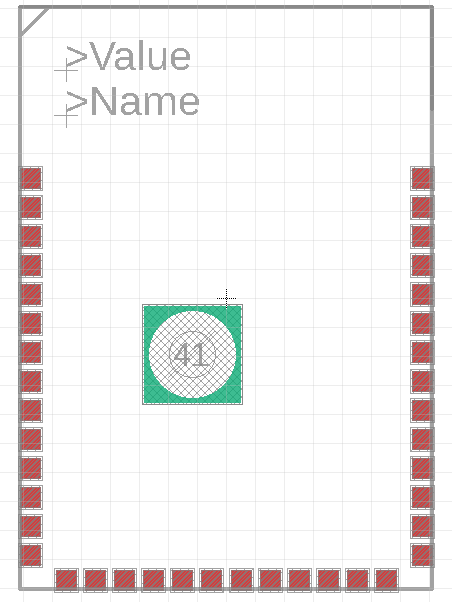
\includegraphics[width=0.7\textwidth]{imagenes/Capitulos/Cap13/ESP32S3HOLE.png}
    \caption{Imagen de la ESP32S3 modificada}
\end{figure}\label{fig:ESP32S3HOLE}

\section{PCB}\label{ApendicePCB}

\subsection{dimenesiones Fisicas}
Dado que el proyecto se va a realizar en una placa de madera, y esta contenga todos los elementos, y que la placa de madera va a ser fresada con una fresadora CNC, se ha decidido dejar margenes de 1mm en cada lado de la placa. Además de añadir un margen extra a la \gls{PCB} para que pueda ser atornillada más facilmente.

En la figura \ref{fig:PlanoSeparacionMadera} podemos ver en rojo el borde de la \gls{PCB} y la línea más próxima, en negro, la madera. Se ha dejado medio milímetro de margen para las máquinas \gls{CNC} y de fabricación de \gls{PCB}. Los marcadores de los interruptores generados por el software de la sección \ref{CreacionPlanoDistribucion} se ha dejado en verde.

\begin{figure}[H]
    \centering
    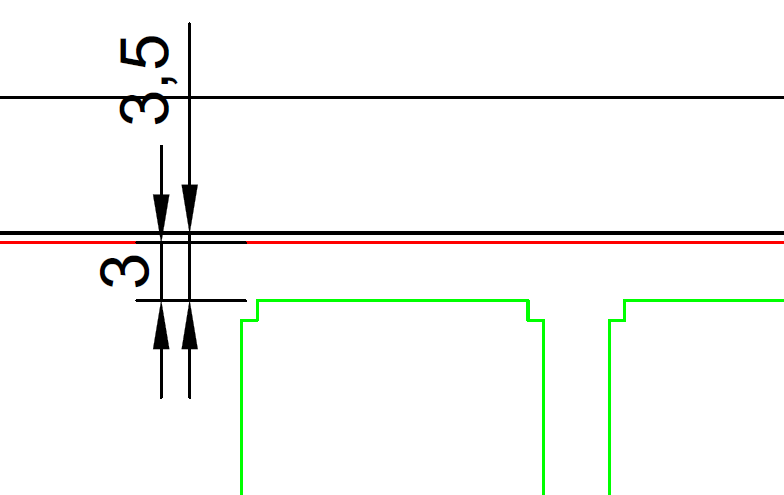
\includegraphics[width=0.8\textwidth]{imagenes/Capitulos/Cap05/AcotadoPCBMadera.png}
    \caption{Imagen del plano acotado del espacio entre las \glsnocase{Keycaps} y la madera.}
    \label{fig:PlanoSeparacionMadera}
\end{figure}

Tambien la idea siempre ha sido ajustar las dimensiones de la carcasa y \gls{PCB} para que no se viera la \gls{PCB} una vez que el teclado tuviese las \glsnocase{Keycaps} puestas, esto ya que al no haber \glsnocase{Plate} si dejaramos mucho hueco, esta parte se veria peor esteticamente. Por eso uno de los objetivos es intentar que la carcasa este lo más cerca de las \glsnocase{Keycaps}.
\newpage

\section{Programación}
\subsection{Codigo fuente}\label{ApendiceCodigoFuente}
\subsection{PID y VID}\label{ApendicePIDVID}
\subsection{Leds}\label{ApendiceLeds}
\subsection{Macros}\label{ApendiceMacros}

\section{Pruebas}\label{ApendicePruebas}
%Pruebas de programacion
Durante el desarrollo del proyecto, se han realizado diversas pruebas para verificar el correcto funcionamiento de los distintos componentes y módulos utilizados. Estas pruebas han sido fundamentales para identificar y corregir errores, así como para garantizar la calidad y fiabilidad del sistema final. En esta sección, se incluyen los detalles de las pruebas realizadas, así como los resultados obtenidos y las conclusiones derivadas de los mismos.

Durante todo el desarrollo se ha ido programando y probando el código en la placa de desarrollo ESP32S3. Se han realizado pruebas de los distintos componentes. El princpial modulo que se ha estado probando ha sido el modulo de la pantalla \gls{OLED} y el Multiplexor. La pantalla ha sido lo que más tiempo ha estado en desarrollo, ya que habia que hacer que funcionase con todos los estados del teclado. Asi mismo, esta tenia que ir cambiando de estado segun el estado del teclado. Por lo que cualquier error en las coordenadas o en la escritura de la pantalla se notaba facilmente y se podia corregir.

Para poder realizar la tarea de actualizar la pantalla se han ido ideando una serie de variables a lo largo del codigo que no indicarian donde esta el estado del teclado, asi podriamos desde cualquier parte del codigo saber en que estado se encuentra el teclado y poder actualizar la pantalla en consecuencia.

Dado que el entorno que teniamos para las pruebas no constaba de un teclado normal. Se decidio crear unas funciones de DEBUG que nos premitirian, mediante el serial de la placa de desarrollo, simular la pulsacion de las teclas. De esta forma podriamos probar el funcionamiento de la pantalla sin necesidad de tener un teclado conectado. Asi como el funcionamiento de la bateria, el bluetooth, etc. Y poder ir cambiando las variables de estado del teclado.

Como podemos ver en el codigo \ref{code:CodigoDebug} esta es la solucion que se ha optado y tambien se puede encontrar en el github del proyecto \cite{ModernWoodGitHub}. 

\begin{lstlisting}[style=console, language=bash, caption={Código de debug para la placa de desarrollo}, label={code:CodigoDebug}]
    #ifdef DEBUG
        // For debug purposes show how many times the loop is executed per second
        loop_counter++;
        if (millis() - last_loop_time > 1000)
        {
            Serial.print("Loop executed ");
            Serial.print(loop_counter);
            Serial.println(" times per second");

            Serial.print("Temperature: ");
            float result = 0;
            temp_sensor_read_celsius(&result);
            Serial.print(result);
            Serial.println(" C");

            loop_counter = 0;
            last_loop_time = millis();

            secs++;
            Serial.print("Seconds: ");
            Serial.println(secs);
        }

        // Read from serial
        char c = 'N';
        if (Serial.available())
        {
            c = Serial.read();
            Serial.print("Read from serial: ");
            Serial.println(c);
        }
        // wasd -> ARRIBA ABAJO DERECHA IZQUIERDA
        // Espace -> Enter
        // E -> Escape
        // Q -> MODO ESPECIAL
        switch (c)
        {
        case 'Q':
            WorkingAsKeyboard = !WorkingAsKeyboard;
            interrupted_FN = true;
            break;

        case 'E':
            MenuPressed[ArrEsc] = true;
            break;

        case ' ':
            MenuPressed[ArrEnter] = true;
            break;

        case 'W':
            MenuPressed[ArrUp] = true;
            break;

        case 'S':
            MenuPressed[ArrDown] = true;
            MenuPressed[ArrDown] = true;
            break;

        case 'A':
            MenuPressed[ArrLeft] = true;
            break;

        case 'D':
            MenuPressed[ArrRight] = true;
            break;

        case '1':
            batteryLevel--;
            batteryLevelChanged = true;
            break;

        case '2':
            batteryLevel++;
            batteryLevelChanged = true;
            break;

        case '3':
            connectionChanged = true;
            isUSBPreferred = !isUSBPreferred;
            isBLEPreferred = !isBLEPreferred;
            break;

        case '4':
            connectionChanged = true;
            isBLEConnected = !isBLEConnected;
            break;

        default:
            break;
        }

    #endif
\end{lstlisting}

\section{Ensamblaje}\label{ApendiceEnsamblaje}
\subsection{Errores}\label{ApendiceEnsamblajeErrores}

\section{Documentación}\label{ApendiceDocumentacion}


%
%%\nocite{*}
%\bibliographystyle{miunsrturl}
%
\appendix
%\input{apendices/manual_usuario/manual_usuario}
%\input{apendices/paper/paper}
%\newglossaryentry{DIY}{
    name={DIY},
    description={Hace referencia a "Do It Yourself" (Hazlo tú mismo). Se trata de la práctica de crear, construir o reparar cosas por uno mismo, en lugar de comprarlas prefabricadas. Es una filosofía que fomenta la creatividad, la autonomía y la satisfacción personal a través de la realización de proyectos artesanales}
}

\newglossaryentry{Keycaps}{
    name={Keycaps},
    description={Se refiere a las tapas individuales de las teclas de un teclado. Estas tapas, a menudo personalizables, pueden tener diferentes diseños, colores o materiales para proporcionar una experiencia de escritura única y estética}
}

\newglossaryentry{Dongle}{
    name={Dongle},
    description={Un dongle es un dispositivo de hardware que se conecta a otro para proporcionar funcionalidad adicional. Comúnmente, se utiliza para referirse a pequeños dispositivos que permiten la conexión inalámbrica o la adaptación de interfaces, como un dongle USB para conectividad Bluetooth}
}

\newglossaryentry{USB}{
    name={USB},
    description={Siglas de ``Universal Serial Bus`` (Bus Universal en Serie). Es un estándar de conexión que permite la transferencia de datos y la conexión de dispositivos electrónicos, como impresoras, cámaras y dispositivos de almacenamiento, a través de un cable estándar}
}

\newglossaryentry{PS2}{
    name={PS2},
    description={Se refiere al conector y protocolo de conexión utilizado comúnmente en teclados y ratones. Aunque ha sido ampliamente reemplazado por conexiones USB, el término PS/2 todavía se utiliza para referirse a dispositivos más antiguos o a sistemas compatibles con este estándar}
}

\newglossaryentry{Bluetooth}{
    name={Bluetooth},
    description={Una tecnología de comunicación inalámbrica de corto alcance que permite la transmisión de datos entre dispositivos electrónicos. El Bluetooth se utiliza comúnmente para la conexión de dispositivos como auriculares, altavoces, teclados y ratones sin necesidad de cables}
}

\newglossaryentry{Vintage}{
    name={Vintage},
    description={Se refiere a objetos, productos o estilos que tienen una cierta edad y que son considerados clásicos o representativos de una época pasada. En el contexto de la tecnología, se utiliza para describir dispositivos antiguos que tienen un atractivo nostálgico o colección}
}

\newglossaryentry{QWERTY}{
    name={QWERTY},
    description={El qwerty es un nombre que se le da a una disposición de las teclas del teclado de las máquinas de escribir que fue patentado en 1878 por Christopher Sholes. Fue el inventor de la máquina de escribir y el precursor del teclado moderno que conocemos hoy en día}
}

\newglossaryentry{Hot-Plugging}{
    name={Hot-plugging},
    description={La capacidad de conectar o desconectar un dispositivo mientras el sistema está en funcionamiento sin necesidad de reiniciar}
}

\newglossaryentry{ISO}{
    name={ISO},
    description={Organización Internacional de Normalización, una entidad que establece estándares para asegurar la calidad y la eficiencia de productos y servicios}
}

\newglossaryentry{Windows}{
    name={Windows},
    description={Un sistema operativo desarrollado por Microsoft que es ampliamente utilizado en computadoras personales}
}

\newglossaryentry{Linux}{
    name={Linux},
    description={Un sistema operativo de código abierto basado en el kernel Linux y utilizado en una variedad de dispositivos, desde servidores hasta dispositivos embebidos}
}

\newglossaryentry{Firmware}{
    name={Firmware},
    description={Software de bajo nivel almacenado en la memoria de hardware que proporciona control básico para los componentes del dispositivo}
}

\newglossaryentry{Ion de litio}{
    name={Ion de Litio},
    description={Un tipo de tecnología de batería recargable comúnmente utilizada en dispositivos electrónicos debido a su alta densidad de energía}
}

\newglossaryentry{Plug-and-Play}{
    name={Plug-and-Play},
    description={La capacidad de un sistema para reconocer automáticamente e instalar dispositivos sin intervención del usuario}
}

\newglossaryentry{Controladores}{
    name={Controladores},
    description={Software que permite la comunicación entre el sistema operativo y el hardware, permitiendo que los dispositivos funcionen correctamente}
}

\newglossaryentry{TTL}{
    name={TTL},
    description={(Transistor-Transistor Logic) también se utiliza para referirse a un programador USB, que permite cargar nuevo firmware en dispositivos. Este programador puede ser empleado en otros proyectos de "bare bones Arduino" o como una interfaz serie USB a TTL de propósito general. Proporciona una conexión y comunicación serial para la programación y configuración de dispositivos electrónicos}
}


\newglossaryentry{LED}{
    name={LED},
    description={Diodo Emisor de Luz, un dispositivo semiconductor que emite luz cuando una corriente eléctrica pasa a través de él}
}

\newglossaryentry{HID}{
    name={HID},
    description={Interfaz Humano-Computadora, un protocolo que permite la comunicación entre dispositivos de entrada, como teclados y ratones, y la computadora}
}

\newglossaryentry{PCB}{
    name={PCB},
    description={Placa de Circuito Impreso, un componente que proporciona conexiones eléctricas entre varios componentes en dispositivos electrónicos}
}

\newglossaryentry{Fresado}{
    name={Fresado},
    description={Un proceso de fabricación que utiliza una herramienta de corte rotativa para dar forma a materiales como metal o plástico}
}

\newglossaryentry{Latencia}{
    name={Latencia},
    description={El tiempo que tarda un sistema en responder a una solicitud después de recibirla, a menudo asociado con retrasos en la transmisión de datos}
}

\newglossaryentry{Switches}{
    name={Switches},
    description={Los switches son los mecanismos debajo de cada tecla de un teclado que detectan cuándo se presiona una tecla y envían la señal al dispositivo electrónico}
}

\newglossaryentry{Plate}{
    name={Plate},
    description={En el contexto de los teclados personalizados o mecánicos, un "plate" se refiere a una pieza de material (como metal, plástico o acrílico) que se coloca debajo de las teclas y sobre la placa base del teclado. El plate proporciona rigidez estructural al teclado y determina la disposición física de las teclas. Además de su función estructural, el diseño del plate también puede afectar la sensación táctil y la respuesta de las teclas al ser presionadas, lo que lo convierte en un componente importante para los entusiastas de los teclados personalizados}
}

\newglossaryentry{Online}{
    name={Online},
    description={En el contexto de la tecnología y la informática, "Online" se refiere a la condición de estar conectado a Internet o a una red informática. Cuando un dispositivo está "online", puede comunicarse con otros dispositivos o acceder a recursos en la red, como sitios web, servicios en la nube, aplicaciones en línea, etc}
}

\newglossaryentry{CNC}{
    name={CNC},
    description={Son las siglas en inglés de "Control Numérico por Computadora" (Computer Numerical Control). Se refiere a un sistema automatizado de control de máquinas herramienta, como fresadoras, tornos y cortadoras láser, mediante el uso de un programa computarizado. Los sistemas CNC son capaces de ejecutar operaciones de mecanizado de alta precisión basadas en instrucciones digitales, lo que los hace indispensables en la fabricación moderna}
}

\newglossaryentry{Deep Sleep}{
    name={Deep Sleep},
    description={En el contexto de los microcontroladores y sistemas embebidos, "Deep Sleep" (sueño profundo) es un modo de bajo consumo de energía diseñado para minimizar el consumo de energía cuando el dispositivo no está activamente realizando tareas. Durante el sueño profundo, el microcontrolador reduce su consumo de energía al mínimo al apagar la mayoría de sus funciones y circuitos, permitiendo que el dispositivo permanezca en un estado de reposo prolongado hasta que se activa por una interrupción externa, como una señal de temporizador o una entrada de sensor. Esta funcionalidad es fundamental en aplicaciones de bajo consumo de energía, como dispositivos portátiles, sensores remotos y sistemas alimentados por batería, donde se busca maximizar la vida útil de la batería o minimizar la dependencia de fuentes de energía externas}
}

\newglossaryentry{WiFi}{
    name={WiFi},
    description={Es una tecnología de comunicación inalámbrica que permite la conexión a Internet y la red de computadoras sin la necesidad de cables físicos. Utiliza ondas de radio de alta frecuencia para transmitir datos entre dispositivos, como computadoras, teléfonos inteligentes, tabletas y dispositivos de red, dentro de un área determinada llamada "zona de cobertura WiFi"}
}

\newglossaryentry{IoT}{
    name={IoT},
    description={Son las siglas en inglés de "Internet of Things" (Internet de las cosas). Se refiere a la red de dispositivos físicos que están integrados con sensores, software y otros componentes tecnológicos que les permiten conectarse y intercambiar datos a través de Internet. Estos dispositivos pueden incluir desde electrodomésticos y dispositivos portátiles hasta vehículos y equipos industriales. La tecnología IoT permite la recopilación, monitorización y control remoto de datos en tiempo real, lo que ofrece una amplia gama de aplicaciones en diversos sectores, como el hogar inteligente, la salud, la agricultura, la industria, la logística y la ciudad inteligente, entre otros}
}

\newglossaryentry{Arduino}{
    name={Arduino},
    description={Es una plataforma de hardware y software de código abierto diseñada para facilitar el desarrollo de proyectos electrónicos interactivos. Consiste en una placa de circuito impreso con un microcontrolador y un entorno de desarrollo integrado (IDE) que simplifica la programación y la interacción con los componentes electrónicos. Arduino es ampliamente utilizado por aficionados, estudiantes y profesionales para crear una amplia variedad de dispositivos y sistemas, desde simples proyectos de bricolaje hasta complejas aplicaciones de automatización y robótica}
}

\newglossaryentry{PlatformIO}{
    name={PlatformIO},
    description={Es un entorno de desarrollo integrado (IDE) de código abierto para el desarrollo de software embebido y aplicaciones IoT. Proporciona herramientas y funcionalidades para escribir, compilar, depurar y cargar código en una variedad de plataformas de hardware, incluyendo Arduino, ESP8266, ESP32, Raspberry Pi y muchas otras. PlatformIO ofrece una interfaz unificada y fácil de usar que facilita el desarrollo y la gestión de proyectos de hardware y software en múltiples plataformas, lo que lo convierte en una opción popular entre los desarrolladores de sistemas embebidos y de IoT}
}

\newglossaryentry{Wearable}{
    name={Wearable},
    description={Dispositivo electrónico vestible que se lleva encima o se incorpora en la ropa y que tiene capacidades de computación y conectividad. Los wearables suelen estar diseñados para monitorizar datos relacionados con la salud, el fitness, la ubicación, entre otros, y pueden incluir dispositivos como smartwatches, brazaletes de fitness y gafas inteligentes}
}

\newglossaryentry{Polling}{
    name={Polling},
    description={El polling rate de un teclado se refiere a la frecuencia con la que el teclado envía información al dispositivo al que está conectado. Es medida en hercios (Hz) y representa cuántas veces por segundo el teclado actualiza su estado y envía los datos correspondientes al dispositivo. Un polling rate más alto significa una respuesta más rápida del teclado, lo que puede resultar en una experiencia de usuario más suave y receptiva, especialmente en aplicaciones que requieren una entrada rápida y precisa, como los juegos}
}

\newglossaryentry{LCD}{
    name={LCD},
    description={Son las siglas en inglés de "Liquid Crystal Display" (Pantalla de Cristal Líquido). Se trata de una tecnología de visualización que utiliza cristales líquidos entre dos láminas de material polarizado para producir imágenes. Los LCD son comúnmente utilizados en dispositivos como televisores, monitores de computadora, relojes digitales y paneles de instrumentos de vehículos}
}

\newglossaryentry{OLED}{
    name={OLED},
    description={Son las siglas en inglés de "Organic Light-Emitting Diode" (Diodo Orgánico de Emisión de Luz). Se trata de una tecnología de visualización que utiliza diodos orgánicos para emitir luz y producir imágenes. A diferencia de los LCD, los OLED no requieren retroiluminación, lo que les permite ofrecer colores más vibrantes, negros más profundos y un mejor contraste. Los OLED son utilizados en dispositivos como teléfonos inteligentes, televisores de alta gama y pantallas de dispositivos portátiles}
}

\newglossaryentry{TFT}{
    name={TFT},
    description={Son las siglas en inglés de "Thin-Film Transistor" (Transistor de Película Fina). Se refiere a una tecnología de pantalla que utiliza transistores de película delgada para controlar cada píxel de la pantalla de manera individual. Los paneles TFT son comúnmente utilizados en pantallas de cristal líquido (LCD) para mejorar la calidad de imagen, aumentar la velocidad de respuesta y permitir una mayor variedad de colores. Los TFT son ampliamente utilizados en dispositivos como monitores de computadora, televisores y pantallas de dispositivos móviles}
}

\newglossaryentry{Multiplexor}{
    name={Multiplexor},
    description={Un multiplexor es un dispositivo electrónico que permite seleccionar una de varias señales de entrada y conectarla a una única salida. Es comúnmente utilizado en electrónica digital para reducir el número de líneas de control necesarias para seleccionar entre múltiples fuentes de datos}
}

\newglossaryentry{Termoretráctil}{
    name={Termoretráctil},
    description={El termoretráctil es un tipo de material plástico que se contrae cuando se calienta, generalmente mediante el uso de una pistola de calor o una fuente de calor similar. Es ampliamente utilizado en la industria electrónica para proteger y aislar conexiones eléctricas y componentes, proporcionando una capa adicional de resistencia al agua, aislamiento y soporte mecánico},
    text={Termoretráctil}
}

\newglossaryentry{API}{
    name={API},
    description={Una API (Interfaz de Programación de Aplicaciones) es un conjunto de definiciones y protocolos que permiten a los distintos componentes de software comunicarse entre sí. Proporciona una interfaz estandarizada para la interacción entre aplicaciones, permitiendo a los desarrolladores acceder a funciones específicas o datos de un software sin necesidad de conocer los detalles internos de su implementación. Las APIs son ampliamente utilizadas en el desarrollo de software para integrar servicios y funcionalidades de diferentes aplicaciones de manera eficiente y coherente}
}

\newglossaryentry{SMD}{
    name={SMD},
    description={Surface Mounted Device, que en inglés significa dispositivo de montaje superficial y se refiere tanto a una forma de encapsulado de componentes electrónicos, como a los equipos construidos a partir de estos componentes}
}

\newglossaryentry{Footprint}{
    name={Footprint},
    description={Un footprint en el contexto de diseño de PCB se refiere al señalamiento ó ubicación de los pads y otros elementos de conexión en la superficie de la placa de circuito impreso (PCB) para un componente electrónico específico}
}

\newglossaryentry{Ghosting}{
    name={Ghosting},
    description={El ghosting se produce cuando el teclado envía solo un comando al PC tras presionar varias teclas a la vez. Por ejemplo, si pulsamos las teclas S + D + F, manda la tecla “S”, por ser la primera pulsada. Otros teclados no mandan ningún comando cuando pulsamos varias a la vez}
}

\newglossaryentry{EMI}{
    name={EMI},
    description={Interferencia Electromagnética, que se refiere a la interferencia causada por campos electromagnéticos que pueden afectar el funcionamiento de dispositivos electrónicos}
}

\newglossaryentry{PID}{
    name={PID},
    description={Product ID, es un identificador único asignado a un dispositivo USB para identificarlo de manera única entre otros dispositivos conectados al mismo sistema}
}

\newglossaryentry{VID}{
    name={VID},
    description={Vendor ID, que se refiere al identificador de proveedor de un dispositivo USB}
}

\newglossaryentry{BackfeedCurrent}{
    name={Back Feed Current},
    description={Corriente de retroalimentación, que se refiere a la corriente que fluye en sentido contrario a través de un dispositivo o circuito, lo que puede causar daños o interferencias en el sistema},
    text={Back feed Current}
}

\newglossaryentry{Pads}{
    name={Pads},
    description={Son las áreas metálicas en una placa de circuito impreso (PCB) donde se sueldan los componentes electrónicos}
}

\newglossaryentry{EEPROM}{
    name={EEPROM},
    description={Son las siglas en inglés de "Electrically Erasable Programmable Read-Only Memory" (Memoria de sólo lectura programable y borrable eléctricamente). Se trata de un tipo de memoria no volátil que puede ser programada, leída y borrada eléctricamente, lo que la hace ideal para almacenar configuraciones, datos y firmware en dispositivos electrónicos. La EEPROM es ampliamente utilizada en microcontroladores y sistemas embebidos para almacenar información que debe persistir incluso cuando el dispositivo se apaga o reinicia}
}

\newglossaryentry{String}{
    name={String},
    description={En programación, una cadena (string) es una secuencia de caracteres, como letras, números y símbolos, que se utilizan para representar texto o datos en un lenguaje de programación. Las cadenas son un tipo de dato fundamental en la mayoría de los lenguajes de programación y se utilizan para almacenar y manipular información de texto, como nombres, mensajes, direcciones, etc}
}

\newglossaryentry{Int}{
    name={Int},
    description={En programación, "int" es un tipo de dato que se utiliza para representar números enteros, es decir, números sin parte decimal. Dependiendo del lenguaje de programación, el rango de valores que puede almacenar un entero puede variar, pero generalmente se utiliza para representar números enteros positivos y negativos}
}

\newglossaryentry{DEBUG}{
    name={DEBUG},
    description={En programación, "DEBUG" se refiere al proceso de identificar y corregir errores o problemas en el código de un programa. El debugging es una parte fundamental del desarrollo de software y se realiza utilizando herramientas y técnicas especializadas para rastrear, analizar y solucionar problemas en el código}
}
\printglossary
\printnoidxglossaries
\addcontentsline{toc}{chapter}{Glosario}
\listoffigures
\addcontentsline{toc}{chapter}{Indice de figuras}
%\input{Bibliografia/Bibliografia}
\bibliographystyle{plain}
\bibliography{Bibliografia/Bibliografia}
\addcontentsline{toc}{chapter}{Bibliografía}

\chapter*{}
\thispagestyle{empty}

\end{document}
